\documentclass{beamer}
\usetheme{CambridgeUS} % My favorite!
\setbeamercolor{title}{fg=red!80!black,bg=white!90!black}
\newenvironment{conenv}{\only{\setbeamercolor{local structure}{fg=darkred}}}{}
\setbeamercovered{dynamic}
\setbeamertemplate{navigation symbols}{} 
\definecolor{links}{HTML}{2A1B81}
%\hypersetup{colorlinks,linkcolor=,urlcolor=links}
\hypersetup{colorlinks,linkcolor=,urlcolor=blue!70!black}
%\hypersetup{colorlinks,linkcolor=,urlcolor=red!80!black}
\usepackage[utf8]{inputenc}
\usepackage{eurosym}
\usepackage{color}
\usepackage{multirow}
\usepackage{hhline}
\usepackage{amsmath}
\usepackage{fancybox}
%\usepackage{kpfonts}
\usepackage[framemethod=TikZ]{mdframed}
\usepackage{tikz}
\usetikzlibrary{backgrounds}
\usepackage{rotating}
\usepackage[skins]{tcolorbox}
\usepackage[percent]{overpic}
\mathchardef\mhyphen="2D
\setbeamerfont{page number in head/foot}{size=\tiny \bf}
\setbeamercolor{page number in head/foot}{fg=red!80!black}
\setbeamerfont{frametitle}{size=\footnotesize}
%\setbeamertemplate{footline}[frame number]
\usepackage{appendixnumberbeamer}
\usepackage{bbding}
\usepackage{pifont}
\usepackage{graphicx}
\usepackage{booktabs}
\usepackage{array}
\usepackage{calc}
\usepackage{makecell}
\newcommand<>{\superimpose}[2][]{%
    \tikz[overlay, remember picture]{%
        \filldraw#3[fill=white, opacity=0.8] (current page.north west) rectangle (current page.south east);
        %\filldraw#3[fill=white, opacity=0.8] (accent_left.south east) rectangle (current page.south east);
        \node#3[at=(current page.center), rotate =20,line width=0.3mm, #1]
			{\vspace{35pt} #2 \vspace{35pt}};
    }%
}
\newcolumntype{P}[1]{>{\centering\arraybackslash}p{#1}}

\settowidth{\leftmargini}{\usebeamertemplate{itemize item}}
\addtolength{\leftmargini}{\labelsep}    % to move bullets

\addtolength{\textwidth}{0cm}
\DeclareRobustCommand{\frac}[3][0pt]{%
  {\begingroup\hspace{#1}#2\hspace{#1}\endgroup\over\hspace{#1}#3\hspace{#1}}}
%\addtolength{\hoffset}{-4cm}

%General
\newcommand{\breakhere}{\noindent\rule{15cm}{0.4pt}}
\newcommand{\qm}{\textbf{\textcolor{red}{?}}}
\newcommand*\plus{\ensuremath{\texttt{+}}~}
\newcommand*\plusn{\ensuremath{\texttt{+}}}
\newcommand*\hy{\ensuremath{\mbox{-}}}

% Chapter 4
\providecommand{\httwo}{\ensuremath{H_{\mathrm{T,2}}/2}\xspace}
\providecommand{\ptone}{\ensuremath{p_{\mathrm{T,1}}}\xspace}
\providecommand{\pttwo}{\ensuremath{p_{\mathrm{T,2}}}\xspace}
\providecommand{\cme}{$\sqrt{s}$\xspace}
\providecommand{\MadGraphF}{{\textsc{MadGraph5}}\xspace}






% Itemize
\newcommand*\ball{\setbeamertemplate{itemize items}[ball]}
\newcommand*\cir{\setbeamertemplate{itemize items}[circle]}
\newcommand*\tri{\setbeamertemplate{itemize items}[triangle]}

%Colors
%\newcommand*\mycolor{\textcolor{red!80!black}}
%\newcommand*\blue{\textcolor{blue!70!black}}
%\newcommand*\green{\textcolor{green!50!black}}
%\definecolor{auburn}{rgb}{0.07, 0.04, 0.56}
\newcommand*\AN{\textcolor{auburn}}
\newcommand*\yes{\textcolor{red!80!black} {\Checkmark }}
\newcommand*\no{\textcolor{red!80!black} {\XSolidBrush}}
%\definecolor{pink}{rgb}{1.0, 0.11, 0.81}
%spaces
\newcommand{\tab}[1]{\hspace{.2\textwidth}\rlap{#1}}
\newcommand{\itab}[1]{\hspace{.12\textwidth}\rlap{#1}}
%\tcbset{colframe=white,colback=white,nobeforeafter}
\newcommand{\mybox}[2]{{\color{red!80!black}\fbox{\normalcolor#2}}}
\setlength\fboxrule{0.8pt}
%Def
\newcommand{\lumins}{\ensuremath{\mathcal{L}}}

\providecommand{\ptave}{\ensuremath{\langle p_\mathrm{T1,2}\rangle}\xspace}
\providecommand{\bqm}{\ensuremath{\scalebox{1.2}{\textbf{?}}}\xspace}
\providecommand{\RooUnfold} {{\textsc{RooUnfold}}\xspace}
\providecommand{\refe}{\ensuremath{\textcolor{red!80!black}{\bf [REF]}}\xspace}
\providecommand{\HERWIGPP} {{\textsc{herwig++}}\xspace}
\providecommand{\PYTHIAS} {{\textsc{pythia6}}\xspace}
\providecommand{\PYTHIAE} {{\textsc{pythia8}}\xspace}
\providecommand{\POWHEG} {{\textsc{powheg}}\xspace}
\providecommand{\NLOJETPP} {{\textsc{NLOJet++}}\xspace}
\providecommand{\RunDec}{{\textsc{RunDec}}\xspace}
\providecommand{\fastNLO} {{\textsc{fastNLO}}\xspace}
\providecommand{\fastjet} {{\textsc{FastJet}}\xspace}
\providecommand{\mur}{\ensuremath{\mu_r}\xspace}
\providecommand{\muf}{\ensuremath{\mu_f}\xspace}
\providecommand{\alpsmz}{\ensuremath{\alpha_s(M_Z)}\xspace}
\providecommand{\chisq}{\ensuremath{\chi^2}\xspace}
\providecommand{\chisqndof}{\ensuremath{\chi^2/n_\mathrm{dof}}\xspace}
\providecommand{\alps}{\ensuremath{\alpha_S}\xspace}
\providecommand{\alpsmusq}{\ensuremath{\alpha_S(\mu_r^2)}\xspace}
\providecommand{\alpsmzsq}{\ensuremath{\alpha_S(M_Z^2)}\xspace}
\providecommand{\alpsqsq}{\ensuremath{\alpha_S(Q^2)}\xspace}
\providecommand{\alpsmu}{\ensuremath{\alpha_S(\mu_r)}\xspace}
\providecommand{\alpsmz}{\ensuremath{\alpha_S(M_Z)}\xspace}
\providecommand{\alpsq}{\ensuremath{\alpha_S(Q)}\xspace}
\providecommand{\ratio}{\ensuremath{R_{32}}\xspace}
\providecommand{\LHAPDF}{{\textsc{LHAPDF}}\xspace}
\providecommand{\LHAPDFS}{{\textsc{LHAPDF6}}\xspace}
\providecommand{\NF}{\ensuremath{N_F}\xspace}
\providecommand{\Ztwostar}{\ensuremath{\mathrm{Z2}^\star}\xspace}
\newcommand{\hftwo}{\hspace*{\fill}}
\newcommand{\rbthm}{\rule[-2ex]{0ex}{5ex}}
\newcommand{\rbtrr}{\rule[-0.8ex]{0ex}{3.2ex}}
\newcommand*\alpsmzns{\ensuremath{\alpha_S(M_Z)}}
\newcommand*\alpsns{\ensuremath{\alpha_S}}
\newcommand*\httwons{\ensuremath{\mathrm{H_{T,2}}/2}}
\newcommand*\ptavens{\ensuremath{\mathrm{\langle p_\mathrm{T_{1,2}}\rangle}}}
\newcommand*\rations{\ensuremath{\mathrm{R_{32}}}}

\newcommand*\pas{\includegraphics[scale=0.3]{/home/anter/Desktop/Analysis_8/Present_Latex/Pre-approval/Plots/pas_new.png}}
\newcommand*\staru{\ensuremath{\blue{^{*}}}}
\newcommand*\unc{\ensuremath{\blue{^{\#}}}}
\newcommand*\pts{p$^2_{\mathrm{T}}$}
\newcommand*\msd{m$_{\mathrm{SD}}$}
\newcommand*\msds{m$^2_{\mathrm{SD}}$}
\newcommand*\met{E$\mathrm{_{T}^{miss}}$}
\newcommand*\varnd{$\mathrm{N_{2,DDT}^1}$}
\newcommand*\vartau{$\mathrm{\tau_{21}^{DDT}}$}
\newcommand*\varn{$\mathrm{N_{2}^1}$}
\newcommand*\rapa{$\mathrm{|\eta|}$}
\newcommand*\gr{$\mathrm{>}~$}
\newcommand*\ls{$\mathrm{<}~$}
\newcommand{\inv}{$^{\text{-}1}$}



\vspace{15 mm}

\title[Anterpreet Kaur (Ph.D. Defence)] {\normalsize MEASUREMENT OF MULTIJET CROSS-SECTION RATIOS \\IN PROTON-PROTON COLLISIONS WITH THE CMS \\DETECTOR AT THE LHC}

\author[Multijet Cross-Section Ratios]{\blue{Candidate : Anterpreet Kaur~~~} \\ { \normalsize Supervisor : Prof. Manjit Kaur}\\}
\vspace{-3mm}
\institute[]
{
%{ \normalsize \blue{Supervisor : Prof. Manjit Kaur }}\\
% \medskip
 %\medskip
 %\medskip
 %\medskip
 Department of Physics \\ Panjab University \\ Chandigarh, India
}
\date[December, 2018]{\footnotesize \textcolor{blue!0!black}{}}

\begin{document}
\setbeamercolor{item}{fg=red!70!black}
\setbeamertemplate{enumerate items}[default]

%###################################### Slide : 1 ######################################
\begin{frame}[plain]
\vspace{0.50mm}
\includegraphics[scale = 0.18]{/home/anter/Desktop/Analysis_8/Present_Latex/Klaus/plots/cms.jpeg}
\hfill
\hspace{50 mm}
\includegraphics[scale = 0.20]{/home/anter/Desktop/Analysis_8/Present_Latex/Klaus/plots/pu.png}
\vspace{0.2mm}
\titlepage
\vspace{2.2mm}
\begin{beamercolorbox}[wd=120mm,ht=1.5mm,center,shadow=true, rounded=true]{redgrey}
{}
{\scriptsize \mycolor{Ph.D. Defence \hfill \hspace{75mm} December , 2018}}
\end{beamercolorbox}
\end{frame}

%###################################### Slide : 2 ######################################
\begin{frame}
\frametitle{\centerline{Outline}}
\setlength\labelsep {\dimexpr\labelsep + 0.05em\relax}
\setlength\leftmargini{\dimexpr\leftmargini + 0.05em\relax}
\begin{itemize}
\item {\scriptsize Physics of the Thesis
\vspace{1mm}
\item Experimental Set-up
\vspace{1mm}
\item Theoretical Background
\vspace{1mm}
\item Software Tools
\vspace{1mm}
\item Analysis Strategy
\vspace{1mm}
\item Measurement of Inclusive Multijet Cross-sections and their Ratio R$_{32}$ 
\vspace{1mm}
\item Theoretical Predictions
\vspace{1mm}
\item Data-Theory Comparisons 
\vspace{1mm}
\item Determination of the Strong Coupling Constant, \alpsmz
\vspace{1mm}
\item Summary
\vspace{1mm}
\item Other Activities\\}
\end{itemize}
\end{frame}

%##################################### Slide : 3 ###########################################
\begin{frame}
\frametitle{\centerline{Physics of the Thesis}}
\setlength\labelsep {\dimexpr\labelsep + 0.05em\relax}
\setlength\leftmargini{\dimexpr\leftmargini + 0.05em\relax}
\vspace{-1.5mm}
\begin{itemize}
\item {\scriptsize Hadrons colliding at very high center-of-mass energies provide a direct probe to the nature of the underlying parton-parton scattering physics.
\vspace{1mm} 
\item {\bf Scattering} \mycolor{$\rightarrow$} {\bf Fragmentation} \mycolor{$\rightarrow$} {\bf Hadronization} \mycolor{$\rightarrow$} {\bf Clustering into Jets}
\vspace{1mm}
\item Jets are the final structures observed in the detector :\\}
\tri
\begin{itemize}
\item {\scriptsize key component to extend our understanding of the Standard Model physics.
\vspace{0.5mm}
\item signatures of large momentum transfers at short distances, belong primarily to perturbative domain of Quantum Chromodynamics (pQCD).
\vspace{0.5mm}
\item relate experimental observations to theory predictions.
\vspace{0.5mm}
\item important backgrounds for many new physics models.\\}
\end{itemize}
\ball 
\item {\scriptsize Inclusive multijet production cross-section provides the details of parton distribution functions (PDF) of the colliding hadrons and precise measurement of the strong coupling constant \alps :\\}
\vspace{-6mm} 
\begin{align*}
\blue{\resizebox{.4\hsize}{!}{$\rm \sigma_{i\mbox{-}jet} = \sigma(pp\to i~jets~\plus X) \propto \alpsns^{i}$}} 
\end{align*}
\item {\scriptsize Cross-sections ratios : ~~~~~\blue{$\rm{R_{mn} = \frac{\sigma_{m\mbox{-}jet}}{\sigma_{n\mbox{-}jet}}} \propto \alpsns^{m-n}~;~ m~>~n$}
\vspace{0mm}
\item {\bf Why cross-section ratios ?} \\
{\bf -} better choice w.r.t. inclusive cross-sections because of less dependency on uncertainties such as : \\}
\begin{itemize}
\tri
\item {\scriptsize uncertainties due to luminosity, 
\vspace{0.2mm}
\item scale dependence, 
\vspace{0.2mm}
\item PDF dependence etc.\\}
\end{itemize}
\ball
%\vspace{0.5mm}
%\item {\scriptsize A measurement of the ratio of the inclusive 3-jet cross-section to the inclusive 2-jet cross-section as a function of the average transverse momentum, $\rm{<p_{T1,2}>}$, of the two leading jets in the event is performed at 7 TeV (\textcolor{red!80!black}{Eur. Phys. J. C 73 (2013) 2604}).\\}
\end{itemize}
\end{frame}

%##################################### Slide : 4 ###########################################
\begin{frame}
\begin{center}
\vspace{13mm}
\textbf{\Large\mycolor{Experimental Set-up}}
\end{center}
\end{frame}

%##################################### Slide : 5 ###########################################
\begin{frame}
\frametitle{\centerline{Large Hadron Collider}}
\setlength\labelsep {\dimexpr\labelsep + 0.05em\relax}
\setlength\leftmargini{\dimexpr\leftmargini + 0.05em\relax}
\begin{itemize}
\item {\scriptsize World’s biggest and the most powerful particle accelerator and collider built by CERN (European Organization for Nuclear Research). 
\vspace{2mm}
\item Located in a 27 km long tunnel, 100 m (approx.) underground at Swiss-France border. \\}
\end{itemize}
\begin{minipage}[thbp]{0.6\textwidth}
\begin{itemize}
\vspace{-6mm}
\item {\scriptsize \blue{\bf Proton-proton (p-p)}, proton-lead and lead-lead as well as xenon-xenon nuclei collisions take place at different center-of-mass energies (\cmens).\\
\vspace{2mm}
{\bf - 3.5 TeV} per beam in 2010 and 2011\\
{\bf - 4.0 TeV} per beam in 2012 \\ 
{\bf - 6.5 TeV} per beam 2015 onwards.
\vspace{2mm}
\item Four big experiments located at \\ different interaction points.\\
\vspace{2mm}
{\bf - ATLAS \& CMS :} General purpose \\
{\bf - ALICE \& LHCb :} Dedicated \\}
\item[]\item[]\item[]
\end{itemize}
%\hspace{5mm}
\end{minipage}
\hspace{-24mm}
\begin{minipage}[thbp]{0.08\textwidth}
\begin{itemize}
\item[]\item[]\item[]
\end{itemize}
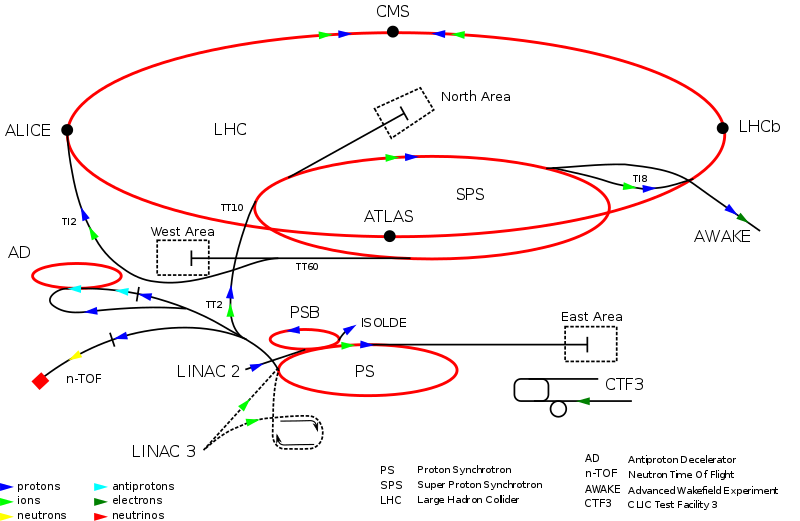
\includegraphics[scale = 0.26]{/home/anter/Desktop/Thesis/Figures/LHC.png}\\
\end{minipage}
\end{frame}

%##################################### Slide : 6 ###########################################
\begin{frame}
\frametitle{\centerline{CMS Detector}}
\setlength\labelsep {\dimexpr\labelsep + 0.05em\relax}
\setlength\leftmargini{\dimexpr\leftmargini + 0.05em\relax}
\vspace{-1mm}
\begin{itemize}
\item {\scriptsize Compact Muon Solenoid (CMS) : One of the general purpose detectors which \\ %located at the interaction point 5 (P5) of the main LHC ring, near the village of Cessy in France. \\
\vspace{1mm}
- is \mycolor{compact} in size : 21 m long, 15 m wide and 15 m high weighing 12,500 tonnes \\
\vspace{0.5mm}
- emphasis on the detection of \mycolor{muons} \\
\vspace{0.5mm}
- is enclosed within high \mycolor{solenoidal} magnetic field \\
\vspace{0.5mm}
\item Complex layered structure of sub-detectors : Tracker, Electromagnetic Calorimeter (ECAL), Hadron Calorimeter (HCAL) and Muon System.\\}
\end{itemize}
\vspace{-3mm}
\begin{center}
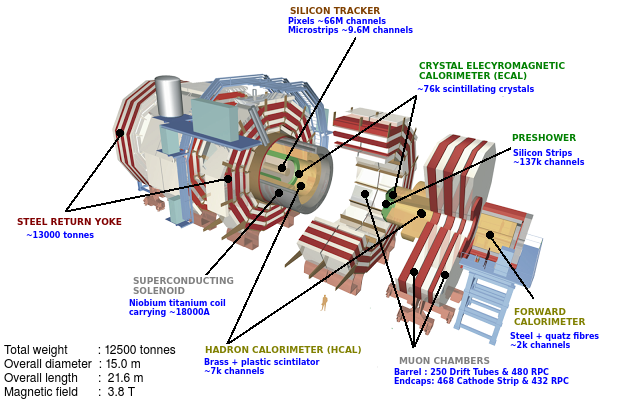
\includegraphics[scale = 0.52]{/home/anter/Desktop/Thesis/Figures/CMS_2_new.png}\\
\end{center}
\end{frame}

%##################################### Slide : 7 ###########################################
\begin{frame}
\frametitle{\centerline{CMS Detector : Front View}}
\setlength\labelsep {\dimexpr\labelsep + 0.05em\relax}
\setlength\leftmargini{\dimexpr\leftmargini + 0.05em\relax}
\begin{minipage}[thbp]{0.45\textwidth}
\begin{itemize}
\item {\scriptsize Major fraction of the particles \\ produced in p-p collisions is hadrons.
\vspace{1mm}
\item Collimated in the form of conical structures called \mycolor{Jets}.
\vspace{1mm}
\item Both hadronic (charged and neutral) and electromagnetic components.
\vspace{1mm}
\item \mycolor{Charged Particles :} energy deposits \\ in the calorimeters.
\vspace{1mm}
\item \mycolor{Neutral Particles :} missing transverse energy.
\vspace{1mm}
\item \mycolor{HCAL :} detects neutral particles; \\an essential sub-system of the CMS detector and contributes to most of physics studies with CMS.\\}
\end{itemize}
\end{minipage}
\hspace{-5.5mm}
\begin{minipage}[thbp]{0.3\textwidth}
\begin{center}
\vspace{-3mm}
\begin{overpic}[scale = 0.48]{/home/anter/Desktop/Thesis/Figures/cropped_CMS_Front.pdf}
\put(34,-3){\tiny $\odot$ - Direction of magnetic field in the return yoke}
\put(34,-6.5){\tiny $\otimes$ - Direction of magnetic field inside the solenoid}
\end{overpic}
\end{center}
\end{minipage}
\end{frame}

%##################################### Slide : 8 ###########################################
\begin{frame}
\frametitle{\centerline{Luminosity Measurement}}
 \setlength\labelsep {\dimexpr\labelsep + 0.05em\relax}
\setlength\leftmargini{\dimexpr\leftmargini + 0.05em\relax}
\vspace{-2mm}
\begin{itemize}
\item {\scriptsize \mycolor{Luminosity ($\mathcal{L}$)} gives the rate at which collisions occur.
\vspace{1mm}
\item Number of collisions produced in a detector per cm$^2$ and per second.\\}
\vspace{1mm}
%\item \lumi~is related to total number of events $N$ of a process over a time period $T$ and $\sigma$ as :\\}
\end{itemize}
\vspace{-2mm}
\begin{align*}
\resizebox{.28\hsize}{!}{$\blue{{\ensuremath N} = \int_{0}^{T} \mathcal{L}~\sigma~dt = \mathcal{L}_{int}~\sigma}$}
\end{align*}
{\scriptsize where $\int_{0}^{T} \mathcal{L}~dt~=~\mathcal{L}_{int}$ gives the total integrated luminosity, expressed in barn$^{-1}$ units\mycolor{$^{*}$}\\}
\vspace{1mm}
\begin{itemize}
\item {\scriptsize $\mathcal{L}_{int}$ gives a direct indication of number of events produced in a process.\\}
\vspace{1mm}
\tri
\begin{itemize}
\item {\scriptsize For e.g. an integrated luminosity of 10 \fbinv~means that 10 events are produced in a process having cross-section equal to 1 fb.\\}
\end{itemize}
\end{itemize}
\ball
\vspace{-2mm}
\begin{minipage}[thbp]{0.53\textwidth}
\begin{itemize}
\item {\scriptsize CMS constantly monitors the instantaneous luminosity delivered by the LHC.
\vspace{0.5mm}
\item The absolute luminosity is measured using van-der-Meer scans done in special runs of the LHC. 
\vspace{0.5mm}
\item The measured integrated luminosity for 2012 data set is \mycolor{19.7 \fbinv$~\pm~ ^{2.5\% (syst.)}_{0.5\% (stat.)}$}\\}
\item[] 
\end{itemize}
{\tiny \mycolor{$^{*}$1 barn = 10$^{-28}~m^2$}\\}
\end{minipage}
\begin{minipage}[thbp]{0.33\textwidth}
\vspace{1mm}
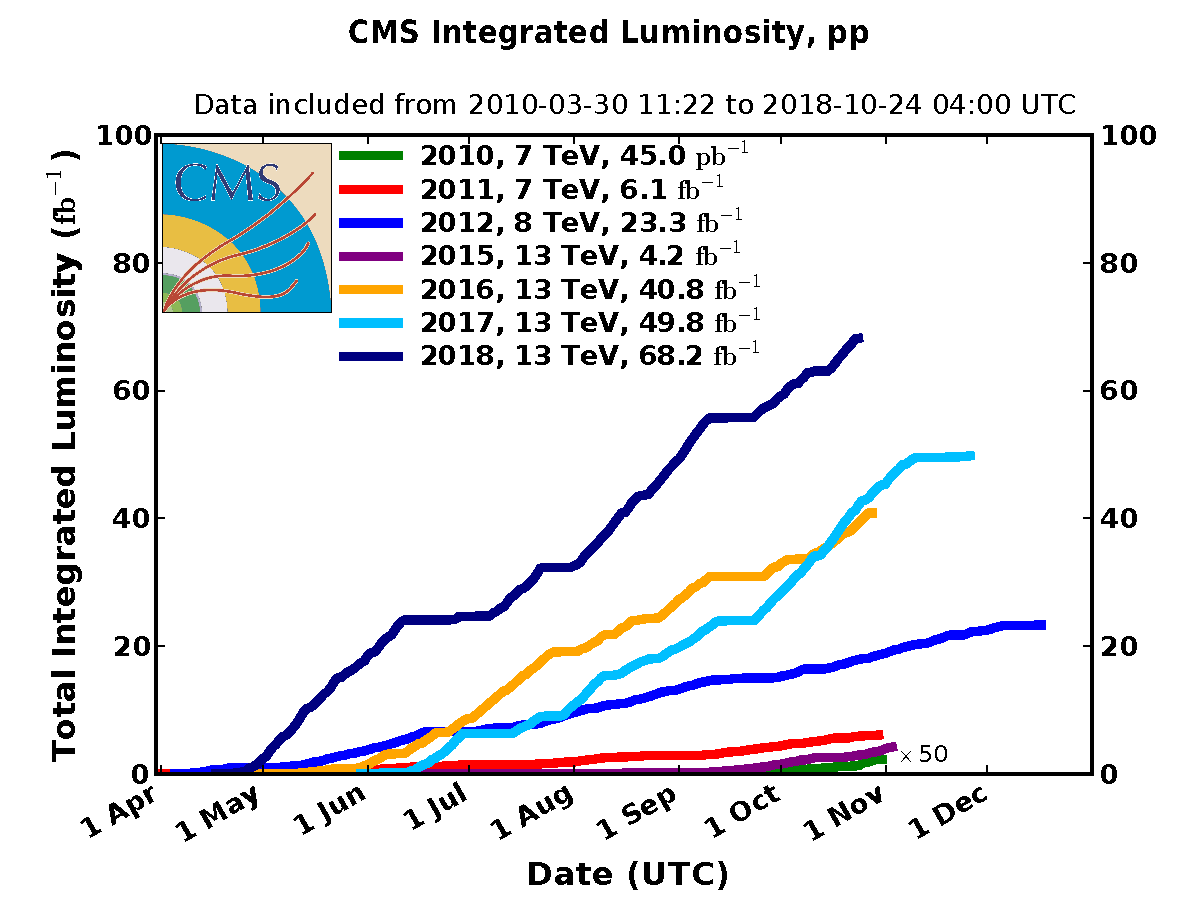
\includegraphics[scale=0.28]{/home/anter/Desktop/Thesis/Figures/int_lumi_cumulative_pp_2_New.pdf}\\
\end{minipage}\\
\end{frame}

%##################################### Slide : 9 ###########################################
\begin{frame}
\begin{center}
\vspace{13mm}
\textbf{\Large\mycolor{Theoretical Background}}
\end{center}
\end{frame}

%##################################### Slide : 10 ###########################################
\begin{frame}
\frametitle{\centerline{Standard Model}}
\setlength\labelsep {\dimexpr\labelsep + 0.05em\relax}
\setlength\leftmargini{\dimexpr\leftmargini + 0.05em\relax}
\begin{itemize}
\item {\scriptsize A theoretical model to describe the nature and properties of fundamental particles and their interactions. \\}
\end{itemize}
\begin{minipage}[thbp]{0.5\textwidth}
\begin{itemize}
\vspace{1mm}
\item {\scriptsize \mycolor{Fundamental particles : \\}}
\tri
\begin{itemize}
\item {\scriptsize Fermions \\}
\cir
\begin{itemize}
\item {\scriptsize Quarks ($q$)
\vspace{1mm}
\item Leptons (\sln) \\}
\end{itemize}
\tri
\item {\scriptsize Bosons \\}
\cir
\begin{itemize}
\item {\scriptsize Gauge Bosons
\vspace{1mm}
\item Scalar Boson \\}
\end{itemize}
\end{itemize}
\ball
%\vspace{1mm}
\item {\scriptsize \mycolor{Forces of interactions : \\}}
\tri
\begin{itemize}
\item {\scriptsize Electromagnetic - photon ($\gamma$) 
\vspace{1mm}
\item Strong - gluons ($g$)
\vspace{1mm}
\item Weak - $W^\pm$ and $Z$
\vspace{1mm}
\item Gravity\mycolor{$^\star$} - graviton}\\
\end{itemize}
\ball
%\item {\scriptsize Described by {\bf SU(3)$_{\rm C}~\otimes$ SU(2)$_{\rm L}~\otimes$ U(1)$_{\rm Y}$} gauge symmetry \\}
\end{itemize}
\vspace{1mm}
\end{minipage}
\hspace{-6mm}
\begin{minipage}[thbp]{0.5\textwidth} 
\begin{overpic}[scale=0.75]{/home/anter/Desktop/Thesis/Figures/model-physics.pdf}\\
\put(30,-12){\tiny \mycolor{{$^\star$}not been incorporated into Standard Model yet}\\}
\end{overpic}
\end{minipage}\\
\begin{itemize}
\vspace{-2mm}
\item {\scriptsize Described by {\bf ${\rm \underbrace{SU(3)_C}_\text{\blue{Strong}}~\otimes \underbrace{SU(2)_L~\otimes U(1)_Y}_\text{\blue{ElectroWeak}}}$} gauge symmetry \\}
\end{itemize}
\vspace{-2mm}
\end{frame}

%##################################### Slide : 11 ###########################################
\begin{frame}
\frametitle{\centerline{Quantum Chromodynamics (QCD)}}
\setlength\labelsep {\dimexpr\labelsep + 0.05em\relax}
\setlength\leftmargini{\dimexpr\leftmargini + 0.05em\relax}
\begin{itemize}
\item {\scriptsize A non-abelian gauge theory describing the strong interactions between quarks and gluons. 
\vspace{1mm}
\item \mycolor{Color charge -} \\}
\tri
\begin{itemize}
\item {\scriptsize Quarks and gluons : colored
\vspace{2mm}
\item Hadrons - Baryons ($qqq$) and Mesons ($q\bar{q}$) : colorless \\}
\end{itemize}
\ball
\item {\scriptsize \mycolor{Strong coupling constant \alps -} a fundamental parameter giving the strength of interaction. \\}
\end{itemize}
\begin{minipage}[thbp]{0.55\textwidth}
\begin{itemize}
\item {\scriptsize \mycolor{Properties - }\\}
\tri
\begin{itemize}
\item {\scriptsize Confinement : at low energies $\rightarrow$ \blue{Non-perturbative (NP) regime}
\vspace{1mm}
\item Asymptotic freedom : at high energies $\rightarrow$ \blue{Perturbative regime} \\}
\end{itemize}
\ball
\item {\scriptsize In perturbative QCD \\}
\end{itemize}
\hspace{5mm}{\scriptsize \blue{$ X = \sum\limits_{i=0}^{N} \alpha^n_s {\rm c}_i = {\rm c}_0~\plus \alpha^1_s {\rm c}_1~\plus \alpha^2_s {\rm c}_2~\plus ... \\$}}
\end{minipage}
\hspace{8mm}
\begin{minipage}[thbp]{0.3\textwidth}
\vspace{4mm}
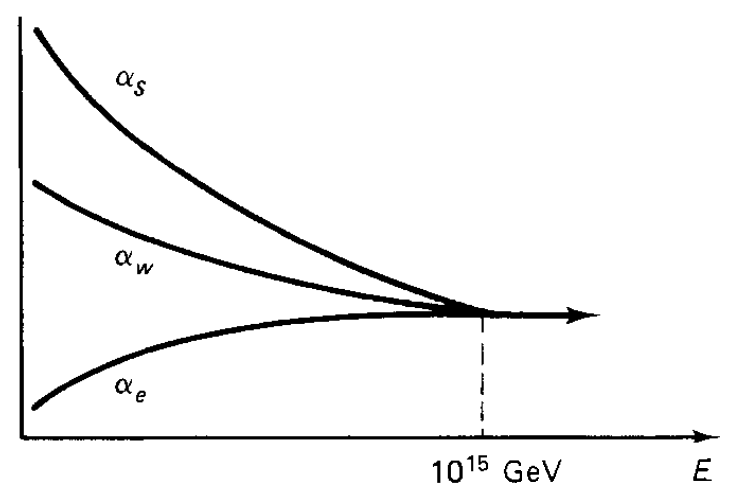
\includegraphics[width=1.3\textwidth]{/home/anter/Desktop/Thesis/Figures/Final/Grifiths.png}
\end{minipage}\\
\hspace{4mm}{\scriptsize is determined by summing over the amplitudes of all Feynman diagrams.\\}
\begin{itemize}
\item[]
\begin{itemize}
\tri
\item {\scriptsize Power of \alps : the number of vertices associated with $q$-$g$ or $g$-$g$ interactions.\\}
\end{itemize}
\end{itemize}
\ball
\end{frame}

%##################################### Slide : 12 ###########################################
\begin{frame}
\frametitle{\centerline{Perturbative QCD}}
\setlength\labelsep {\dimexpr\labelsep + 0.05em\relax}
\setlength\leftmargini{\dimexpr\leftmargini + 0.05em\relax}
\begin{center}
\begin{overpic}[scale = 0.5]{/home/anter/Desktop/Thesis/Figures/Orders.pdf}
\vspace{-3mm}
\put(20,49){\scriptsize \mycolor{\bf Different orders in a 2 $\rightarrow$ 2 scattering process}}
\put(90,5){\tiny \mycolor{\bf \alpsq = $g^2_s/4\pi$}}
\end{overpic}
\begin{itemize}
\item {\scriptsize \mycolor{Ultraviolet (UV) divergences :} Calculations become complex with the loop diagrams; associated integrals are divergent. %- the momenta of the virtual particles in a loop are not fully constrained by four-momentum conservation
\item \mycolor{Renormalization :} a mathematical procedure which \\}
\begin{itemize}
\tri 
\item {\scriptsize allows finite calculation of momenta integrals of virtual loop by removing UV divergences.
\vspace{0.5mm}
\item introduces a regulator for the infinities - \blue{renormalization scale \mur}.
\vspace{0.5mm}
\item redefines or renormalizes the coupling constant to absorb the UV divergences. \\}
\end{itemize}
\end{itemize}
\ball
\end{center}
\end{frame}

%##################################### Slide : 13 ###########################################
\begin{frame}
\frametitle{\centerline{Running of the Strong Coupling}}
\setlength\labelsep {\dimexpr\labelsep + 0.05em\relax}
\setlength\leftmargini{\dimexpr\leftmargini + 0.05em\relax}
\vspace{-.5mm}
\begin{minipage}[thbp]{0.6\textwidth}
\begin{itemize}
\item {\scriptsize \mycolor{Renormalization group equation (RGE)} : exact dependence of \alpsmusq on \mur\\}
\tri
\begin{itemize}
\item {\scriptsize Dependence of $X$ on \mur~must cancel $\rightarrow$ \\ \begin{center} \hspace{4mm}\blue{$\mur^{2}\frac{d}{d\mur^{2}}X\Big(\frac{Q^{2}}{\mur^{2}},\alpha_{s}(\mur^{2})\Big)=0$}\end{center}
\vspace{0mm}
\item First order solution of RGE is : \\ 
\begin{center} \hspace{4mm} \blue{$\alpha_{s}(\mur^2)=\frac{1}{b_0~{\rm ln}\big(\mur^2/\Lambda^2_{QCD}\big)}$} \end{center}
\vspace{0mm}
\item Coupling becomes large at the scale $\Lambda_{QCD}$
\vspace{1mm}
\item For $b_0$ \gr 0, coupling becomes weaker at higher scales $Q$ $\rightarrow$ \mycolor{asymptotic freedom} \\}
\end{itemize}
\end{itemize}
\end{minipage}
\hspace{-2.5mm}
\begin{minipage}[thbp]{0.3\textwidth}
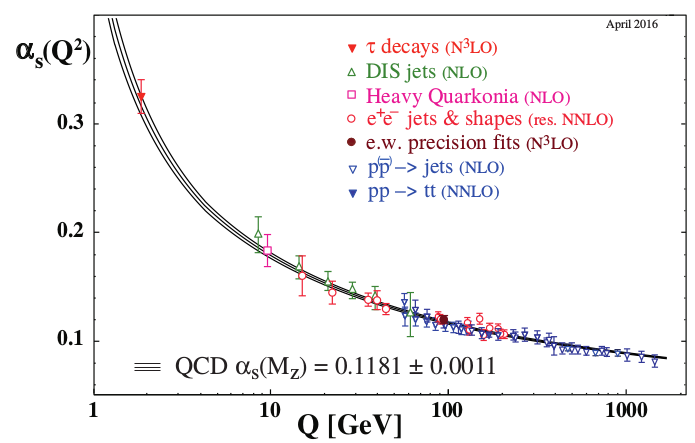
\includegraphics[scale=0.23]{/home/anter/Desktop/Thesis/Figures/Final/Alpha.png}
\end{minipage}
\begin{itemize}
\ball
\vspace{1mm}
\item {\scriptsize It is always convenient to express \alps at some fixed scale - \\}
\tri
\begin{itemize}
\item {\scriptsize Some of the best measurements come from $Z$ decays : the strong coupling is determined at the \mycolor{scale of the $Z$ boson mass \alpsmzns} given by \\}
\end{itemize}
\begin{center}
{\scriptsize\blue{$\alpsns\big(\mur,\alpsmzns\big) = \frac{\alpsmz}{1~\plus \alpsmzns b_0{\rm ln}(\mur^2/M^2_z)}$}\\}
\end{center}
\ball
\item {\scriptsize \alps: a free parameter of QCD theory \\}
\tri
\begin{itemize}
\item {\scriptsize must be extracted from experimental measurements 
\vspace{0.5mm}
\item evolved to the scale of the $Z$ boson
\vspace{0.5mm}
\item current world average value\mycolor{$^\star$}is \blue{$\alpsmz = 0.1181 \pm 0.0011$}\\}
\end{itemize}
\ball
\end{itemize}
\hfill {\tiny \mycolor{{$^\star$}Particle Data Group (PDG)}\\}
\end{frame}

%##################################### Slide : 14 ###########################################
\begin{frame}
\frametitle{\centerline{Hadronic Collisions}}
\setlength\labelsep {\dimexpr\labelsep + 0.05em\relax}
\setlength\leftmargini{\dimexpr\leftmargini + 0.05em\relax}
\begin{minipage}[thbp]{0.6\textwidth}
\begin{itemize}
\item {\scriptsize \mycolor{Proton} - three valence quarks ($uud$), gluons and the sea quarks. 
%\item At large momentum transfer, the collision between two hadrons can be visualized as an interaction between their constituents - $q$ and $g$.
\item \mycolor{Cross-section ($\sigma$)} of a certain process : the probability that the two hadrons interact and give rise to that final state. 
\item In a hadronic collision, the perturbation theory is only valid at the parton-level. %but due to property of confinement at low energies, free partons cannot exist in nature. 
\item \mycolor{Factorization theorem} - allows the calculation of $\sigma$ by separating into two parts : \\}
{\scriptsize $\sigma_{P_1P_2 \rightarrow X}=\blue{\sum\limits_{i,j}^{}\int_{}^{} dx_1dx_2f_{i,P_1}(x_1,\muf)f_{j,P_2}(x_2,\muf)}$}~\\{\scriptsize \hspace{15mm}$\times~\green{\hat\sigma_{ij\rightarrow X} \Bigg(x_1p_1,x_2p_2,\alpha(\mur^2),\frac{Q^2}{\muf^2}\Bigg)}$} \\
\tri
\end{itemize}
\end{minipage}
\hspace{-2mm}
\begin{minipage}[thbp]{0.35\textwidth}
\begin{overpic}
[scale=0.26]{/home/anter/Desktop/Thesis/Figures/Factorization_3.pdf}\\
\put(62,26){\tiny{\green{a short-distance}}}
\put(58,22){\tiny{\green{partonic cross-section}}}
\put(58,18){\tiny{\green{calculable with pQCD}}}
\put(30,80){\tiny{\blue{a NP long-distance part described}}} 
\put(32,76){\tiny{\blue{by parton distribution functions}}}
\put(47,71){\tiny{\blue{$f_i(x,\muf)$ (PDFs)}}}
\end{overpic}\\
\end{minipage}
\tri
\begin{itemize}
\item[]
\begin{itemize}
\item {\scriptsize Proton PDFs {\bf $f_i$} and {\bf $f_{j}$} : probability to find a parton $i$ with momentum fraction $x$ within a hadron.
\item \mycolor{Factorization scale, \muf} : corresponds to the resolution with which the hadron is being probed. \\}
\cir
\begin{itemize}
\item {\scriptsize Particles emitted with \mycolor{\pt~\gr \muf} are considered in the calculation of hard scattering perturbative coefficients. 
\item Particles emitted with \mycolor{\pt~\ls \muf} are accounted for within the PDFs.\\}
\end{itemize}
\end{itemize}
\end{itemize}
\end{frame}
\ball

%##################################### Slide : 15 ###########################################
\begin{frame}
\frametitle{\centerline{Hadronic Collisions}}
\setlength\labelsep {\dimexpr\labelsep + 0.05em\relax}
\setlength\leftmargini{\dimexpr\leftmargini + 0.05em\relax}
\begin{center}
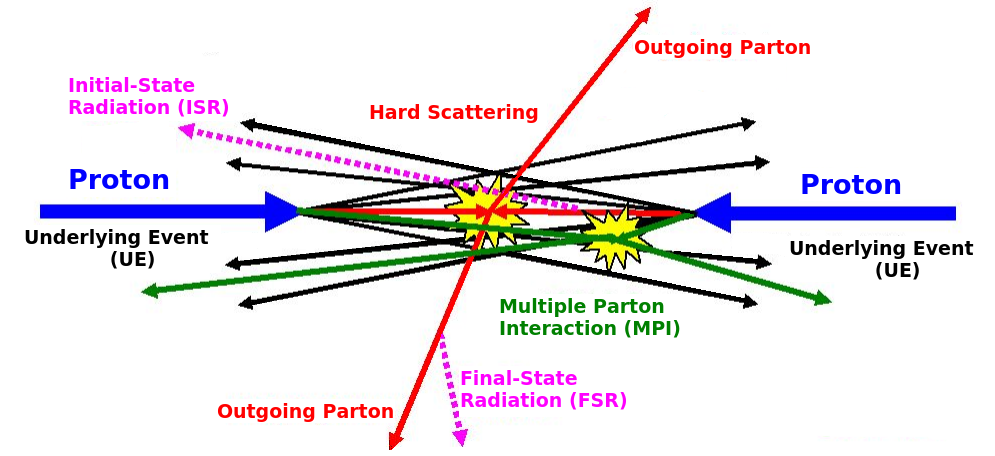
\includegraphics[scale=0.28]{/home/anter/Desktop/Thesis/Figures/MPI.png}\\

\begin{itemize}
\item {\scriptsize \red{\bf Hard Scattering :}\\}
\tri
\begin{itemize}
\item {\scriptsize Parton Shower : collinear parton splitting and the soft gluon emissions (pQCD).
\vspace{1mm}
\item Hadronization : confinement of colored quarks and gluons into the color-neutral composite particles called hadrons (non-pQCD).\\}
\end{itemize}
\ball
\item {\scriptsize {\bf Underlying Event :} Event structure is significantly more complex than that of the lepton collisions.\\}
\tri
\begin{itemize}
\item {\scriptsize \textcolor{pink}{\bf Initial and Final-State Radiations (ISR, FSR) :} two incoming as well as outgoing partons can also develop parton showers.
\vspace{1mm}
\item \green{\bf Multiple Parton Interactions (MPI) :} remaining two partons which do not participate in a hard collision may also interact.\\ }
\end{itemize}
\end{itemize}
\end{center}
\end{frame}

%##################################### Slide : 16 ###########################################
\begin{frame}
\frametitle{\centerline{Jets}}
\setlength\labelsep {\dimexpr\labelsep + 0.05em\relax}
\setlength\leftmargini{\dimexpr\leftmargini + 0.05em\relax}
\begin{minipage}[thbp]{0.54\textwidth}
\begin{itemize}
\item {\scriptsize Hadrons produced in p-p collisions get collimated \\ in the form of conical structures called ``jets'' of radius `R'. 
\vspace{1mm}
\item Direction of the jet is towards the direction of the initial partons that originated them. 
\vspace{1mm}
\item Detectable objects which relate experimental observations to theory predictions formulated in terms of partons.\\}
\end{itemize}
\end{minipage}
\hspace{-2mm}
\begin{minipage}[thbp]{0.2\textwidth}
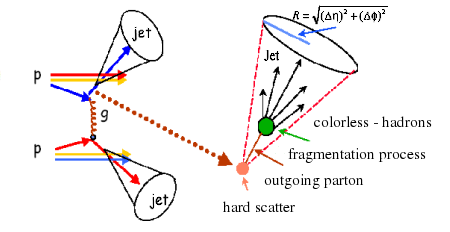
\includegraphics[scale = 0.38]{/home/anter/Desktop/Thesis/Figures/jet2.png}\\
%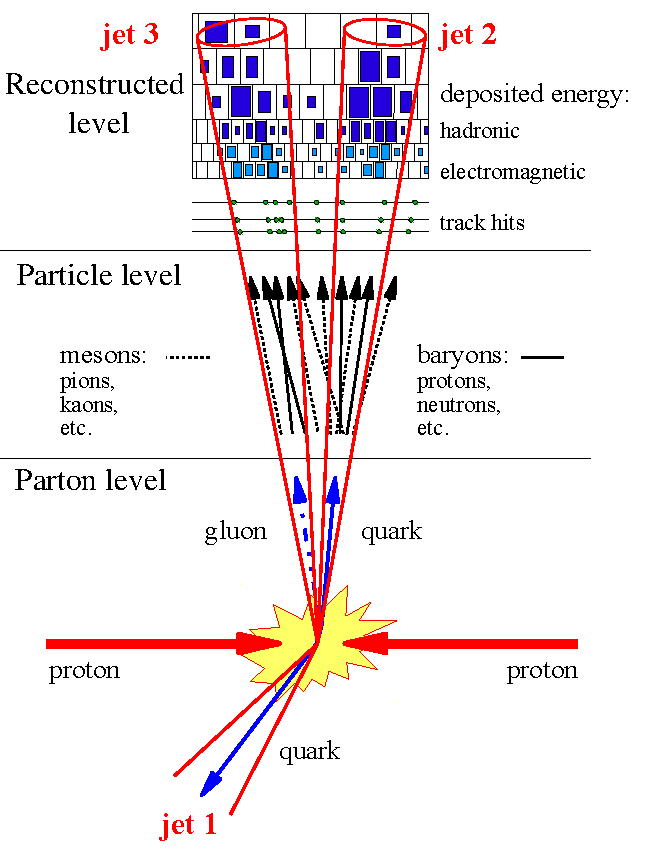
\includegraphics[scale = 0.38]{/home/anter/Desktop/Thesis/Figures/jet_levels_en_edited.pdf}\\
\end{minipage}
\vspace{-2mm}
\begin{itemize}
\item {\scriptsize Act as a bridge between the elementary quarks and gluons of QCD and the final hadrons produced in high energy collisions. 
\vspace{1mm}
\item At the LHC, {\bf Dijet Events} : 2 $\rightarrow$ 2, {\bf Multijet Events :} 2 $\rightarrow$ 3, 2 $\rightarrow$ 4
\vspace{1mm}
\item Jets and their observables are the best tools to test the predictions of pQCD : \\}
\tri
\begin{itemize}
\item {\scriptsize \mycolor{Jet production cross-section :} helps to extract the value of \alps and to reduce the uncertainties of the PDFs of the proton.
\vspace{1mm}
\item Inclusive multijet event cross-sections permits more elaborate tests of QCD.
\vspace{1mm} 
\item A precise study of jet variables helps to understand the signal and background modelling for new physics searches in hadronic final states.\\}
\end{itemize}
\ball
\end{itemize}
\end{frame}

%##################################### Slide : 17 ###########################################
\begin{frame}
\frametitle{\centerline{Jet Algorithms}}
\setlength\labelsep {\dimexpr\labelsep + 0.05em\relax}
\setlength\leftmargini{\dimexpr\leftmargini + 0.05em\relax}
\begin{itemize}
\item {\scriptsize Jet algorithms provide a set of rules which determine how the particles can be clustered into a jet.
\item Parameters involved indicate how close two particles must be to belong to the same jet :\\}
\tri
\begin{itemize}
\item {\scriptsize \mycolor{Cone algorithms} $\rightarrow$ closeness in coordinate space
\vspace{1mm} 
\item \mycolor{Sequential Recombination algorithms} $\rightarrow$ closeness in momentum space\\}
\end{itemize}
\ball
\item {\scriptsize Recombination Scheme \\}
\end{itemize}
\begin{minipage}[thbp]{0.75\textwidth}
%\vspace{-10mm}
\begin{itemize}
\item {\scriptsize \mycolor{Infrared safety : } Addition of a soft emission should not change the number of hard jets found in an event.
\item \mycolor{Collinear safety :} Collinear splitting should not modify the number of jets formed in an event. 
\item Three types of Sequential Recombination algorithms : \\}
\tri
\begin{itemize}
\item {\scriptsize \kt : involves clustering of soft particles first; susceptible to the underlying and pileup events
\item Cambridge/Aachen (C/A) : involves energy independent clusterings.
\item \blue{\bf anti-\kt:} cluster hard particles first; less sensitive to underlying and pileup events.\\}
\end{itemize}
\ball
\end{itemize}
\end{minipage}
\hspace{-2.5mm}
\begin{minipage}[thbp]{0.1\textwidth}
\begin{center}
\vspace{-6mm}
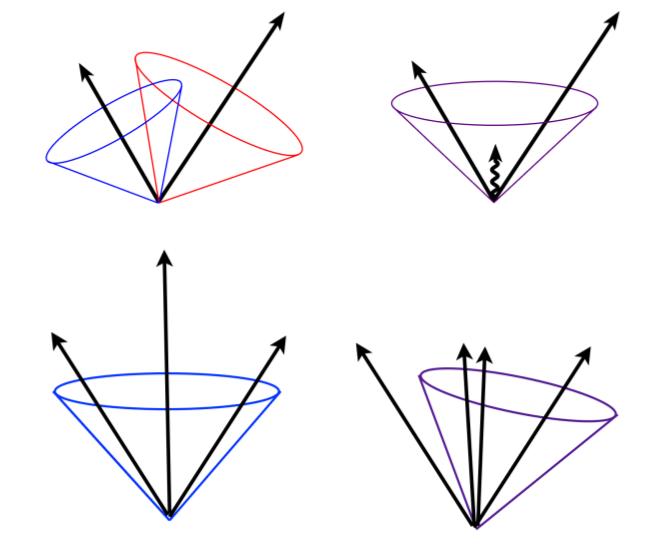
\includegraphics[scale = 0.2]{/home/anter/Desktop/Thesis/Figures/Final/Algo.png}\\
\end{center}
\end{minipage}
\end{frame}

%##################################### Slide : 18 ###########################################
\begin{frame}
\begin{center}
\vspace{13mm}
\textbf{\Large\mycolor{Software Tools}}
\end{center}
\end{frame}

%##################################### Slide : 19 ###########################################
\begin{frame}
\frametitle{\centerline{Software Tools}}
\setlength\labelsep {\dimexpr\labelsep + 0.05em\relax}
\setlength\leftmargini{\dimexpr\leftmargini + 0.05em\relax}
\begin{itemize}
\item {\scriptsize \mycolor{CMS software (CMSSW) framework :} a dedicated data structure and software tools.\\}
\tri
\begin{itemize}
\item {\scriptsize Performs calibration, event generation, detector simulation, event reconstruction etc. by implementing the codes either in C\plusn\plus or Python languages.\\}
\end{itemize}
\ball
\item {\scriptsize \mycolor{ROOT :} an open source object-oriented data analysis framework.\\}
\tri
\begin{itemize}
\item {\scriptsize Consists of a huge C\plusn\plus library which store and analyze large amounts of the data. 
\vspace{0.5mm}
\item Provides histrogramming methods in 1, 2 and 3 dimensions, curve fitting functions, minimization procedures, graphics and visualization classes. \\}
\end{itemize}
\ball
\item {\scriptsize \mycolor{\fastjet :} a software C\plusn\plus package.\\}
\tri
\begin{itemize}
\item {\scriptsize Provides a broad range of jet finding, determination of jet areas, estimation of pileup and underlying-event noise levels etc. \\}
\end{itemize}
\ball
\item {\scriptsize \mycolor{\NLOJET~:} a C\plusn\plus program to evaluate jet production cross-sections at leading order (LO) and next-to-leading order (NLO).\\}
\tri
\begin{itemize}
\item {\scriptsize Calculations of pQCD cross-sections using Monte Carlo integration methods are very time consuming. 
\vspace{0.5mm}
\item PDF fits or estimations of uncertainties becomes difficult where the calculations of the cross-sections are needed to be repeated. \\}
\end{itemize}
\ball
\item {\scriptsize \mycolor{\fastNLO :} fast re-evaluations of cross-sections in interface with \NLOJETPPn. \\}
\tri
\begin{itemize}
\item {\scriptsize The strong coupling constant and the PDFs can be changed without a re-calculation of the perturbative coefficients.\\}
\end{itemize}
\ball
\end{itemize}
\end{frame}

%##################################### Slide : 20 ###########################################
\begin{frame}
\frametitle{\centerline{Monte Carlo (MC) Simulations}}
\setlength\labelsep {\dimexpr\labelsep + 0.05em\relax}
\setlength\leftmargini{\dimexpr\leftmargini + 0.05em\relax}
\begin{itemize}
\item {\scriptsize \mycolor{\PYTHIA :} most widely used program to generate the collisions at high energies.\\}
\tri
\begin{itemize}
\item {\scriptsize Uses LO calculations to derive the colored partons from the hard interaction.
\vspace{0.5mm}
\item Uses the Lund string hadronization model to describe hard and soft interactions and parton showers. 
%\item Uses the Lund string hadronization model to describe hard and soft interactions, PDFs, ISR/FSR parton showers, multi-parton interactions, fragmentation and decay. 
%\item Originally coded in FORTRAN language as \PYTHIASn, and rewritten in C\plusn\plus as \PYTHIAE.
\vspace{0.5mm}
\item \blue{\PYTHIAS with tune \Ztwostar} and \blue{\PYTHIAE~with tunes CUETS1 and CUETM1} have been used.\\}
\end{itemize}
\ball
\item {\scriptsize \mycolor{\MadGraph~:} generates LO matrix elements for high energy physics processes.\\}
\tri
\begin{itemize}
\item {\scriptsize Stores the event information of the particles in the Les Houches format.
\vspace{0.5mm}
\item \blue{\MadGraphFn} has been interfaced to \blue{\PYTHIAS with tune \Ztwostar} - used here mainly for general comparisons to the data and calculating the detector resolution. \\}
\end{itemize}
\ball
\item {\scriptsize \mycolor{\HERWIG~(Hadron Emission Reactions With Interfering Gluons) :} a multi-purpose LO event generator. \\}
\tri
\begin{itemize}
\item {\scriptsize Uses angular ordering for parton showers and cluster model for hadronization.
%\item \HERWIG and \HERWIGPP are written in FORTRAN and C\plusn\plusn languages, respectively.
\vspace{0.5mm}
\item \blue{\HERWIGPP with the default tune of version 2.3} has been used to study the non-perturbative effects.\\}
\end{itemize}
\ball
\item {\scriptsize \mycolor{\POWHEG~(Positive Weight Hardest Emission Generator)} : performs the fixed NLO calculations merged with parton showers.\\}
\tri
\begin{itemize}
\item {\scriptsize Uses \POWHEG~BOX to implement NLO calculations in shower MC programs. 
\vspace{0.5mm}
\item \blue{\POWHEG} has been interfaced to \blue{\PYTHIAE~with tunes CUETS1 and CUETM1} to include the parton shower and hadronization. \\}
\end{itemize}
\ball
\end{itemize}
\end{frame}

%##################################### Slide : 23 ###########################################
\begin{frame}
\begin{center}
\vspace{13mm}
\textbf{\Large\mycolor{Measurement of the Differential Inclusive Multijet \\\vspace{2mm}Cross-sections and their Ratio \ratio}}
\end{center}
\end{frame}

% ###################################### Slide : 24 ######################################
\begin{frame}
\frametitle{\centerline{Analysis Strategy}}
\setlength\labelsep {\dimexpr\labelsep + 0.05em\relax}
\setlength\leftmargini{\dimexpr\leftmargini + 0.05em\relax}
\begin{itemize}
\item {\scriptsize Jets are reconstructed from particle flow objects using the \mycolor{anti-\kt}clustering algorithm with the size parameter \mycolor{R = 0.7}.
\vspace{0.2mm}
\item Event Selection : Appropriate selection criteria has been designed for choosing the best event for analysis. This measurement uses jets with \mycolor{\pt~\gr 150 GeV} and \mycolor{$|y|$ \ls 2.5}.
\vspace{0.2mm}
\item Pileup reweighting.
\vspace{0.2mm}
\item Detector level comparison of differential inclusive 3-jet and 2-jet cross-sections in terms of defined observable for full Data, MC and theory predictions.
\vspace{0.2mm}
\item Unfolding set-up and the measured cross-sections are corrected for detector smearing effects by using the Unfolding technique.
\vspace{0.2mm}
\item Evaluated cross-section ratio, \rations.
\vspace{0.2mm}
\item Evaluated experimental and systematic uncertainties from different sources.
\vspace{0.2mm}
\item Included NLO pQCD calculations obtained using different PDF sets and corrected them for MPI and HAD effects by applying non-perturbative
(NP) corrections as well as for electroweak (EW) effects.
\vspace{0.2mm}
\item Evaluated theoretical uncertainties from different sources.
\vspace{0.2mm}
\item Compared theoretical results with that of data.
\vspace{0.2mm}
\item Extracted the value of \alpsmz by fitting cross-sections as well as cross-section ratio, \rations.
\vspace{0.2mm}
\item Studied the running of \alpsq~as a function of $Q$.\\}
\end{itemize}
\end{frame}

%##################################### Slide : 25 ###########################################
\begin{frame}
\frametitle{\centerline{Multijet Cross-sections and their Ratio \ratio}}
\setlength\labelsep {\dimexpr\labelsep + 0.05em\relax}
\setlength\leftmargini{\dimexpr\leftmargini + 0.05em\relax}
\begin{itemize}
\item {\scriptsize The scale based on the transverse momentum of the jets is used :
\begin{align*}
\blue{\resizebox{.32\hsize}{!}{${\langle p_\mathrm{T_{1,2}}\rangle~} = {\frac{p_{\mathrm T,1}~\plus p_{\mathrm T,2}}{2} = \httwot}$}}
\end{align*}
\item Inclusive differential multijet event cross-section (pb/GeV) is defined as : \\}
\vspace{-5mm}
\begin{align*}
\resizebox{.37\hsize}{!}{$\mycolor{\frac{d\sigma_{{\it n}-{\rm jet}}}{d(\httwotns)} =  \frac{1}{\epsilon~\mathcal{L}_{\mathrm{int,eff}}}\frac{N_\mathrm{event}}{\Delta(\httwotns)}}$} %~~~~\mathrm{where}$}
\end{align*}
\vspace{-3mm}
\item {\scriptsize {\bf Inclusive $n$\hy jet} event samples include the events with {\bf number of jets (\nj) $\geq$ $n$}.\\}
\begin{itemize}
\tri
\item {\scriptsize $n$ = 2 $\rightarrow$ Inclusive 2-jet events \blue{(\njt)}
\item $n$ = 3 $\rightarrow$ Inclusive 3-jet events \blue{(\njth)}\\}
\end{itemize}
\vspace{1mm}
\item {\scriptsize Cross-section ratio is defined as :
\vspace{-3mm}
\begin{align*}
\mycolor{\ratio = \frac[10pt]{{\dd{\sigma_{3\hy {\rm jet}}}{\big(\httwotns\big)}}}{\dd{\sigma_{2\hy {\rm jet}}}{\big(\httwotns\big)}}}
\end{align*}
\item \mycolor{Samples used : }\\}
\begin{itemize}
\tri 
\item {\scriptsize {\bf Data} collected at \cme~= 8 TeV during 2012 run; Integrated Luminosity : \blue{19.7 \fbinv}
\vspace{0.5mm}
\item {\bf Simulated Monte-Carlo (MC)} samples using \MadGraphF \plus \PYTHIAS Tune Z2$^{\star}$ (\MGP~Z2*), \HERWIGPP and \PYTHIAS generators.
\vspace{0.5mm}
\item {\bf Theoretical NLO} calculations using the \blue{\NLOJETPP}program (v4.1.3) within the framework of the \blue{\fastNLO}package (v2.3) using different PDF sets. \\}
\end{itemize}
\end{itemize}
\end{frame}
\ball

%##################################### Slide : 26 ###########################################
\begin{frame}
\frametitle{\centerline{Trigger Studies}}
\setlength\labelsep {\dimexpr\labelsep + 0.05em\relax}
\setlength\leftmarginiii{\dimexpr\leftmarginiii + 0.05em\relax}
\vspace{-1mm}
\begin{minipage}[thbp]{0.55\textwidth} 
\begin{itemize}
\item {\scriptsize CMS implements a two-level trigger system to reduce the amount of recorded events to a sustainable rate.
\item Five {\bf single-jet high-level triggers} : select an event in which at least one jet has the transverse momentum above the threshold.
\vspace{0.5mm}
%\item Only highest-threshold trigger is unprescaled.
%\vspace{0.5mm} 
\item Trigger efficiency for HLT\_PFJetY : \\}
\end{itemize}
\end{minipage}
\hspace{6mm}
\begin{minipage}[thbp]{0.3\textwidth} 
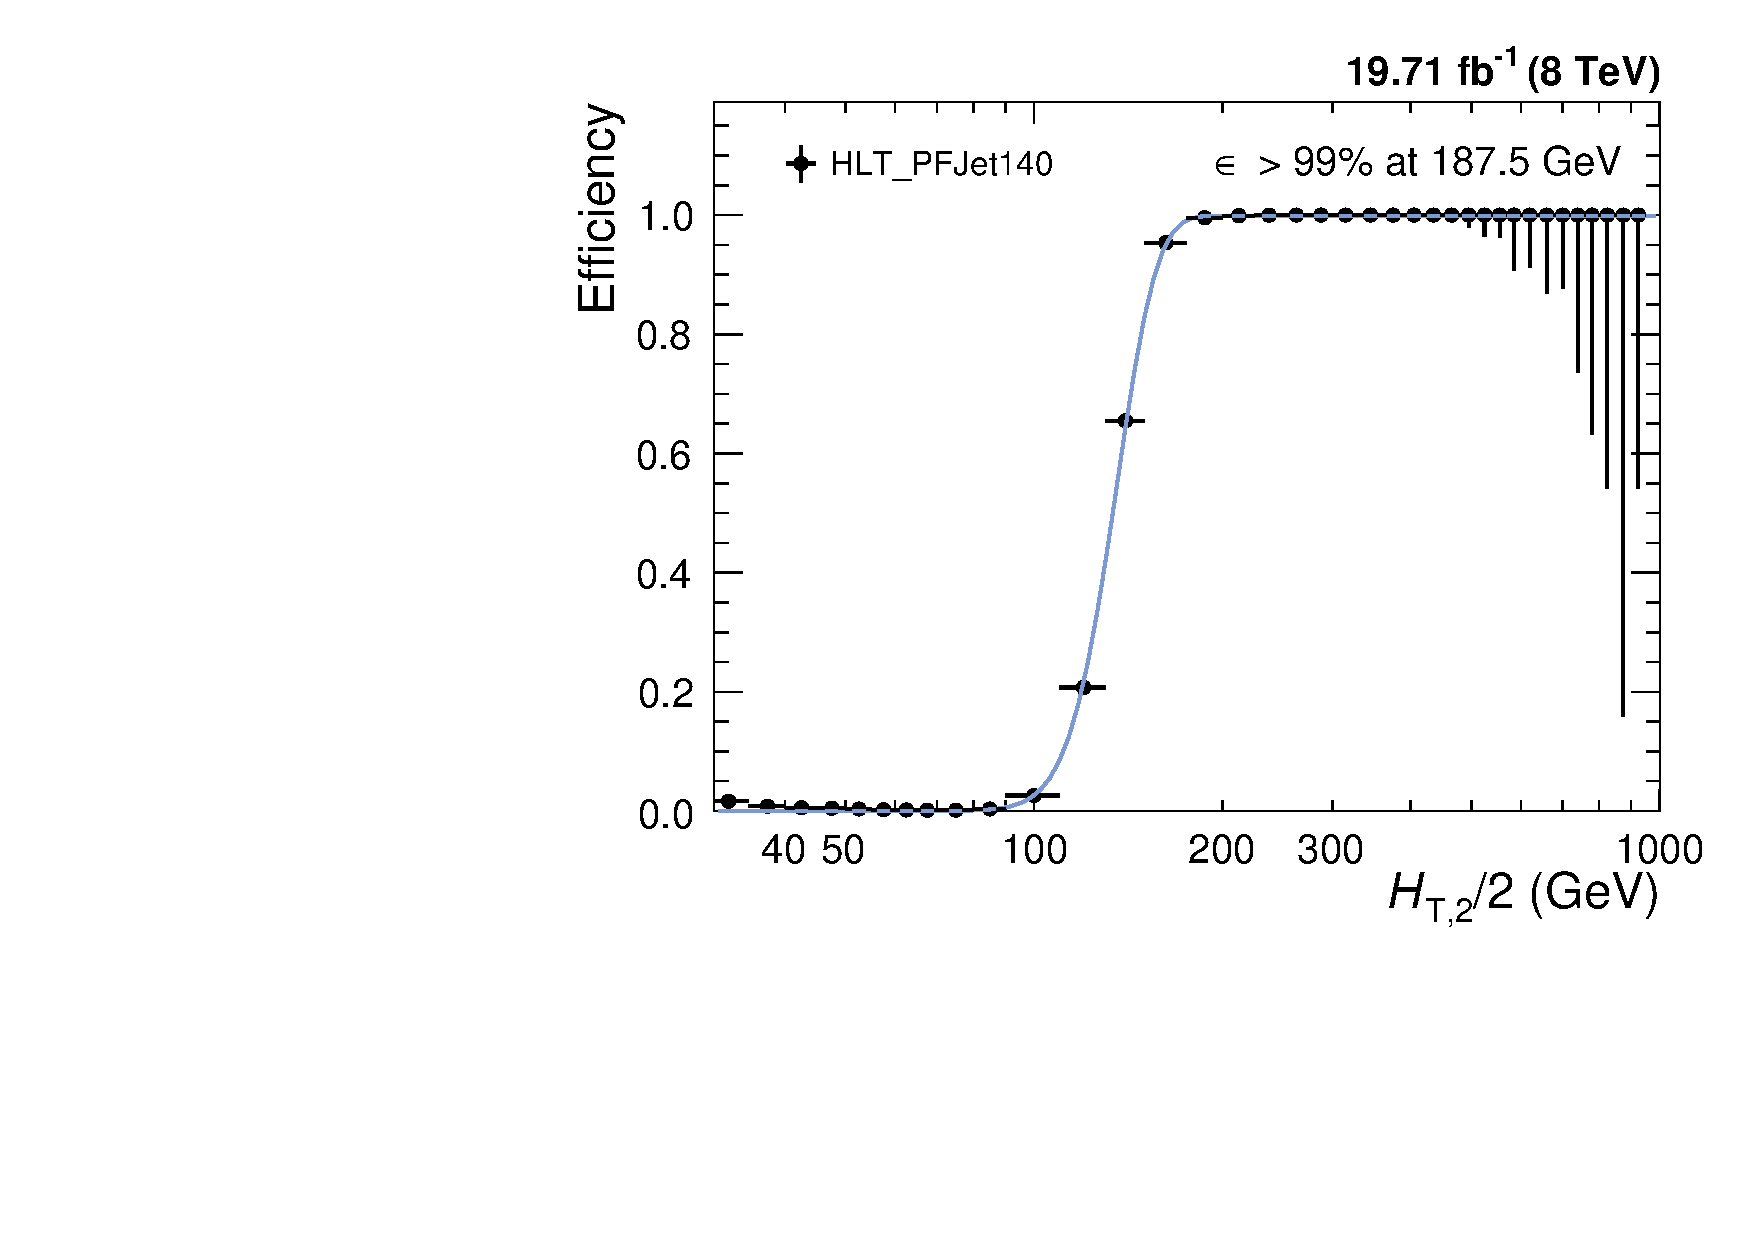
\includegraphics[scale=0.215]{Plots_HT_2_150/Fit_Turn_Efficiency_140_2_ht_2.pdf}
\end{minipage}
\vspace{-1.5mm} 
\begin{align*}
\resizebox{.8\hsize}{!}{\blue{$\rm {\epsilon_{HLT\_PFJetY}} = \frac{\httwotns\big(HLT\_PFJetX~\plus (L1Object\_{p_{\rm T}}~\geq~Z)~\plus (HLTObject\_{p_{\rm T}}~\geq~Y)\big)}{\httwotns\big(HLT\_PFJetX \big)}$}}
\end{align*}
\begin{itemize}
\item[]
\tri
\vspace{-1mm}
\begin{itemize}
\item {\scriptsize the value of X is chosen previous to that of Y in \pt~ordering
\vspace{0.5mm} 
\item Z is the L1 seed value corresponding to the trigger path \\}
\end{itemize}
\ball
\vspace{1mm}
\item {\scriptsize Trigger regions defined as ranges of the \httwot for every single-jet trigger used : \\}
\end{itemize}
\vspace{-1.5mm} 
\begin{table}[htbp]
 %\centering
 \tiny
\begin{tabular}{ccccl}
 \hline\hline
 {\bf Trigger Path} & \makecell{{\bf L1 threshold} \\{\bf (GeV)}} & \makecell{{\bf HLT threshold} \\ {\bf (GeV)}} & \makecell{{\bf \httwotns, 99\%}\\ {\bf (GeV)}} & \makecell{{\bf Eff. Lumi} \\ {\bf (\fbinv)}} \rbthm\\\hline
 HLT\_PFJet80       &  36 &  80 & 120.0 & ~0.0021 \rbtrr \\
 HLT\_PFJet140      &  68 & 140 & 187.5 & ~0.0560 \rbtrr \\
 HLT\_PFJet200      &  92 & 200 & 262.5 & ~0.2600 \rbtrr \\
 HLT\_PFJet260      & 128 & 260 & 345.0 & ~1.0600 \rbtrr \\
 HLT\_PFJet320      & 128 & 320 & 405.0 & 19.7100 \rbtrr \\
 \hline\hline
 \end{tabular}
\end{table}
\end{frame}

%##################################### Slide : 27 ###########################################
\begin{frame}
\frametitle{\centerline{Jet Energy Corrections}}
\setlength\labelsep {\dimexpr\labelsep + 0.05em\relax}
\setlength\leftmargini{\dimexpr\leftmargini + 0.05em\relax}
\begin{itemize}
\item {\scriptsize Measured energy of jets cannot be directly translated to the energy at true particle or parton level.\\} 
\begin{itemize}
\tri
\item {\scriptsize Non-linear and non-uniform response of the calorimeters, effects of pileup and small residual effects in the data remaining after the corrections based on MC simulations.\\}
\end{itemize}
\item {\scriptsize CMS follows a factorized approach : \\}
\end{itemize}
\vspace{-4mm}
\begin{align*}
p^{\rm corr}_{\rm T} = c_{\rm res}(\eta,p''_{\rm T})\cdot c_{\rm mc}(\eta,p'_{\rm T})\cdot c_{\rm pileup}(\eta,\rho,{\rm A}_{j},p^{\rm raw}_{\rm T})\cdot p^{\rm raw}_{\rm T}
\end{align*}
%\begin{center}
\hspace{-3mm}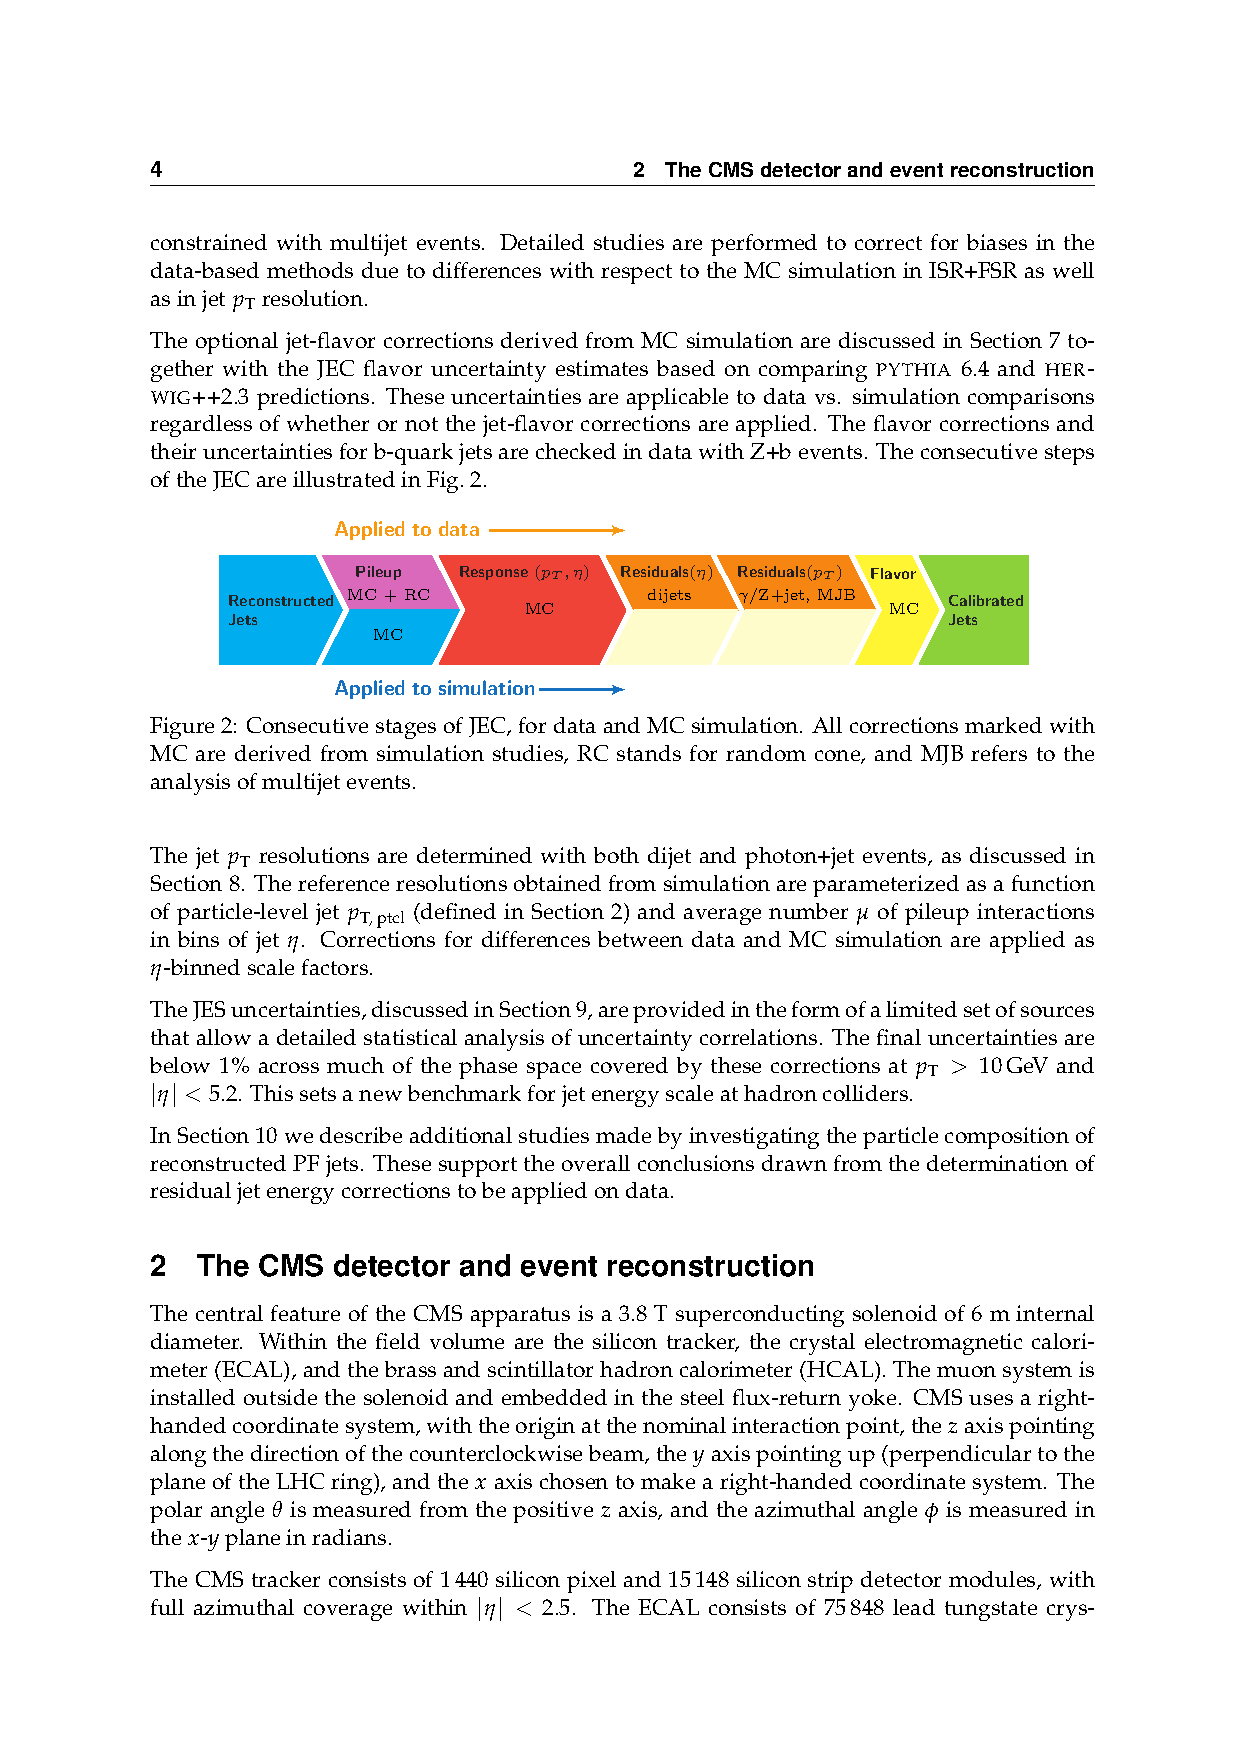
\includegraphics[scale=0.9]{/home/anter/Desktop/Thesis/Figures/New/JEC.pdf}\\
\vspace{3mm}
\begin{itemize}
\item {\scriptsize Corrections are applied to jets in both the data$^{\mycolor{\#}}$ as well as in simulated events$^{\mycolor{*}}$.}\\ {\tiny \green{[Details in Back-up slide~\ref{corr}]}\\}
\end{itemize}
%\end{center}
{\tiny \mycolor{$^{\#}$ Winter\_V8 jet energy corrections}\\}
\vspace{-2mm}
{\tiny \mycolor{$^{*}$ START53\_V27 jet energy corrections}}
\end{frame}

%##################################### Slide : 28 ###########################################
\begin{frame}
\frametitle{\centerline{Pileup Interactions}}
 \setlength\labelsep {\dimexpr\labelsep + 0.05em\relax}
\setlength\leftmargini{\dimexpr\leftmargini + 0.05em\relax}
\noindent
\begin{center}
\begin{itemize}
\item {\scriptsize To observe the extremely rare events, the event rate in a collider should be very high.\\}
\end{itemize}
\vspace{2mm}
{\scriptsize {\bf High delivered luminosity} \\
\vspace{0.5mm}
\mycolor{$\downarrow$} \\
\vspace{0.5mm}
{\bf Increase in the number of bunches or protons per bunch} \\
\vspace{0.5mm}
\mycolor{$\downarrow$} \\
\vspace{0.5mm}
{\bf Pileup (PU) interactions}\\
\vspace{0.5mm}
\mycolor{$\downarrow$} \\
\vspace{0.5mm}
{\bf Low \pt~jets}\\}
\end{center}
\begin{minipage}[thbp]{0.48\textwidth}
\begin{itemize}
\item {\scriptsize {\bf In-time pileup :} Additional collisions within a single bunch crossing.
\vspace{1mm}
\item {\bf Out-of-time pileup :} Additional collisions coming from other bunch crossings.\\}
\end{itemize}
\end{minipage}
\begin{minipage}[thbp]{0.33\textwidth}
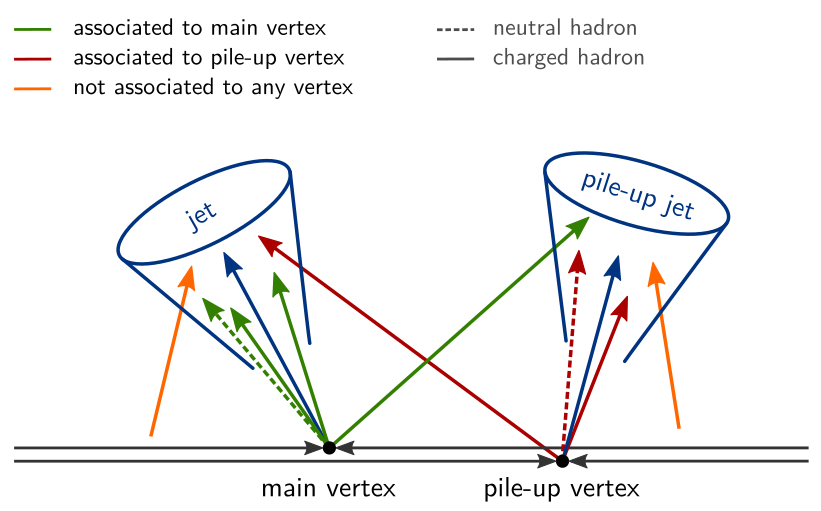
\includegraphics[scale=0.3]{/home/anter/Desktop/Thesis/Figures/Final/Pileup.png}
\end{minipage}
\end{frame}

%##################################### Slide : 29 ###########################################
\begin{frame}
\frametitle{\centerline{Pileup Reweighting}}
 \setlength\labelsep {\dimexpr\labelsep + 0.05em\relax}
\setlength\leftmargini{\dimexpr\leftmargini + 0.05em\relax}
\vspace{-3mm}
\begin{center}
\begin{itemize}
\item {\scriptsize Number of pileup interactions are taken into account in generating the official MC samples. 
\vspace{0.2mm}
\item Pileup implemented in the simulation $N_{\rm MC} (N_{\rm PU,truth})$ does not match exactly the one measured in the data $N_{\rm data} (N_{\rm PU,est.})$. 
\vspace{0.2mm}
\item A reweighting factor $w_{\rm PU}$ is applied to the simulated events : \\}
\end{itemize}
\vspace{-5mm}
\begin{align*}
\blue{\resizebox{.38\hsize}{!}{$ w_{\rm PU} = \frac {N_{\rm data} (N_{\rm PU,est.})/\sum N_{\rm data}} {N_{\rm MC} (N_{\rm PU,truth)}/\sum N_{\rm MC}}$}}
\end{align*}
%\hspace{5mm} \blue{\scriptsize \bf Before Pileup reweighting}
%\hspace{25mm} \blue{\scriptsize \bf After Pileup reweighting}
\vspace{-3.7mm}
\begin{overpic}[scale=0.3]{Plots_HT_2_150/Nvertices.pdf}
\put(72,62){\mycolor{\bf {\footnotesize Before}}}
\end{overpic}%
\begin{overpic}[scale=0.3]{Plots_HT_2_150/Nvertices_weight.pdf}
\put(72,62){\mycolor{\bf {\footnotesize After}}}
\end{overpic}
\end{center}
\end{frame}

%##################################### Slide : 30 ###########################################
\begin{frame}
\frametitle{\centerline{Detector Level Comparisons}}
\setlength\labelsep {\dimexpr\labelsep + 0.05em\relax}
\setlength\leftmarginiii{\dimexpr\leftmarginiii + 0.05em\relax}
%\begin{itemize}
%\item {\scriptsize LO MC generator roughly describes the spectrum on %detector level \\}
%\end{itemize}
\vspace{-1.3mm}
\hspace{33mm}\begin{overpic}[scale = 0.22]{/home/anter/Desktop/Thesis/Viva/Plots_HT_2_150_cropped/cropped_Comparison_all_2_HT_2_150.pdf}
\put(42,82){\mycolor{\bf {\footnotesize 2-jet}}}
\put(-72,60){\parbox{1.08in}{\scriptsize - Data are compared to the sample of {\bf \MGP~Z2*} simulated events.\\}}
\put(-72,26){\parbox{1.08in}{\scriptsize \mycolor{- LO MC generator roughly describes the spectrum on detector level.} \\}}
\end{overpic}%
\begin{overpic}[scale = 0.22]{/home/anter/Desktop/Thesis/Viva/Plots_HT_2_150_cropped/cropped_Comparison_all_3_HT_2_150.pdf}
\put(42,82){\mycolor{\bf {\footnotesize 3-jet}}}
\end{overpic}\\
\begin{minipage}[tbp]{0.55\textwidth}
\begin{itemize}
\item {\scriptsize Cross-section ratio\mycolor{*} \ratio : \\}
\vspace{0.5mm} 
\tri
\begin{itemize}
\item {\scriptsize Numerator and denominator are not independent samples.
\vspace{0.5mm} 
\item Statistical uncertainty is calculated using the \mycolor{Wilson score interval} method which takes into account the correlation between the numerator and the denominator. \\}
\end{itemize}
\end{itemize}
\end{minipage}
\hspace{3mm}
\begin{minipage}[tbp]{0.25\textwidth}
\begin{overpic}[scale = 0.25]{Plots_HT_2_150/Ratio_32_all_HT_2_150.pdf}
\put(42,62){\mycolor{\bf {\footnotesize R$_{32}$}}}
\end{overpic}\\
\end{minipage}\\
\vspace{-7mm}
\mycolor{\tiny *Due to kinematical constraints, the minimum cut on \httwot is 300 GeV.\\}
\end{frame}

%##################################### Slide : 31 ###########################################
\begin{frame}
\frametitle{\centerline{Unfolding}}
\setlength\labelsep {\dimexpr\labelsep + 0.05em\relax}
\setlength\leftmarginiii{\dimexpr\leftmarginiii + 0.05em\relax}
\begin{minipage}[tbp]{0.66\textwidth}
\begin{itemize}
 \item {\scriptsize \mycolor{Jet energy resolution (JER)} : Finite value of the resolution of the detector because of differences of the measured quantity from its true value.\\} %Difference of the measured quantity from its true value due to detector noise, uncertainties in the calibration, non-linearity of the response etc.
\tri
\begin{itemize}
\item {\scriptsize Given by the width of a Gaussian distribution, centered around the true value of the measured quantity. {\tiny \green{[Details in Back-up slides~\ref{jer1}-\ref{jer2}]}}\\}
\end{itemize}
\ball
\item {\scriptsize The finite detector resolution along with the steeply falling jet \pt~spectrum distorts the measured cross-sections. 
%\item Each \pt~bin content contains the migrated events from neighbouring bins along with the original events. 
\item \mycolor{Unfolding} of the data allows direct comparison of experimental measurements with theory predictions or with the results from other experiments.
\item Unfolding uses a {\bf Response Matrix} that maps the true distribution onto the measured one.\\}
\tri
\begin{itemize}
\vspace{1mm}
\item {\scriptsize {\bf Fitting} the theoretically predicted NLO spectrum to get true \httwot spectrum. {\tiny \green{[Details in Back-up slide~\ref{fit_formula1}-\ref{fit_formula2}]}}
\vspace{1mm}
\item {\bf Forward Smearing} is performed using the additionally smeared MC JER to obtain measured \httwot spectrum.\\}
\item []
\end{itemize}
\end{itemize}
\end{minipage}
\hspace{-2mm}
\begin{minipage}[tbp]{0.2\textwidth}
\vspace{-1mm}
\begin{center}
\begin{overpic}[scale = 0.22]{Plots_HT_2_150/Normalized_Response_Matrix_NLO_2_range_column.pdf}
\put(62,22){\mycolor{\bf {\footnotesize 2-jet}}}
\end{overpic}\\
\begin{overpic}[scale = 0.22]{Plots_HT_2_150/Normalized_Response_Matrix_NLO_3_column.pdf}

\put(62,22){\mycolor{\bf {\footnotesize 3-jet}}}
\end{overpic} \\
\end{center}
\end{minipage} 
\ball
\begin{itemize}
\vspace{-1.5mm}
\item {\scriptsize The measurements are unfolded by using the iterative D'Agostini method with {\bf 4 iterations}, implemented in the RooUnfold software package.\\}
\end{itemize}
\end{frame}

%##################################### Slide : 32 ###########################################
\begin{frame}
\frametitle{\centerline{Unfolding}}
\setlength\labelsep {\dimexpr\labelsep + 0.05em\relax}
\setlength\leftmarginiii{\dimexpr\leftmarginiii + 0.05em\relax}
\vspace{-1mm}
\begin{minipage}[tbp]{0.52\textwidth}
\begin{itemize}
\item {\scriptsize \mycolor{Unfolding \ratio :}\\}
\item[] {\scriptsize {\bf - Method I :} First unfold the measured cross-sections separately and then construct \rations.
\item[] {\bf - Method II :} Unfold directly \rations.\\}
\item {\scriptsize \mycolor{Closure test :} \\}
\item[] {\scriptsize - Measured$_{\rm Toy}$ spectrum is unfolded.
\item[] - On Unfolding Reco \MGP~MC, small non-closures observed.
\item[] - Unfolded using the response matrices obtained using 30\% reduced JER.
\item[] - Difference between the two is taken as an additional uncertainty. \\}
\end{itemize}
\end{minipage}
\hspace{-6mm}
\begin{minipage}[tbp]{0.14\textwidth}
\begin{overpic}[scale = 0.16]{Plots_HT_2_150/Extrapolate_Theory_Ratio_32_funcII.pdf}
\put(62,18){\mycolor{\bf {\footnotesize R$_{32}$}}}
\end{overpic}%
\begin{overpic}[scale = 0.16]{Plots_HT_2_150/Normalized_Response_Matrix_NLO_ratio_32_column_3.pdf}
\put(62,18){\mycolor{\bf {\scriptsize R$_{32}$}}}
\end{overpic}\\
\begin{overpic}[scale = 0.16]{Plots_HT_2_150/Ratio_Unfolding_NLO_2_funcI.pdf}
\put(25,18){\mycolor{\bf {\scriptsize 2-jet}}}
\end{overpic}%
\begin{overpic}[scale = 0.16]{Plots_HT_2_150/Comparison_closure_2_range.pdf}
\put(25,18){\mycolor{\bf {\scriptsize 2-jet}}}
\end{overpic}\\
\end{minipage}
\begin{center}
\vspace{-2mm}
\begin{overpic}[scale = 0.18]{Plots_HT_2_150/Ratio_Unfolding_data_NLO_2.pdf}
\put(25,18){\mycolor{\bf {\scriptsize 2-jet}}}
\end{overpic}%
\begin{overpic}[scale = 0.18]{Plots_HT_2_150/Ratio_Unfolding_data_NLO_3.pdf}
\put(25,18){\mycolor{\bf {\scriptsize 3-jet}}}
\end{overpic}%
\begin{overpic}[scale = 0.18]{Plots_HT_2_150/Ratio_Unfolding_data_NLO_ratio32.pdf}
\put(25,18){\mycolor{\bf {\scriptsize R$_{32}$}}}
\end{overpic}\\
\end{center}
\end{frame}

%##################################### Slide : 33 ###########################################
\begin{frame}
\frametitle{\centerline{Experimental Uncertainties}}
\setlength\labelsep {\dimexpr\labelsep + 0.05em\relax}
\setlength\leftmargini{\dimexpr\leftmargini + 0.05em\relax}
\vspace{-3mm}
\begin{center}
\begin{overpic}[scale = 0.25]{Plots_HT_2_150/Total_unc_all_2_NLO_add.pdf}
\put(25,18){\mycolor{\bf {\footnotesize 2-jet}}}
\end{overpic}%
\hspace{4mm}
\begin{overpic}[scale = 0.25]{Plots_HT_2_150/Total_unc_all_3_NLO_add.pdf}
\put(25,18){\mycolor{\bf {\footnotesize 3-jet}}}
\end{overpic}\\
\end{center}
\vspace{-2mm}
\begin{minipage}[tbp]{0.4\textwidth}
\vspace{-6mm}
\begin{table}[t]
  %\centering
  \tiny
   %\begin{tabular}{cccc}
   \vspace{-8mm}
   \begin{tabular}{ >{\arraybackslash}m{0.6in} >{\arraybackslash}m{0.53in} >{\arraybackslash}m{0.53in} >{\arraybackslash}m{0.55in}}
    \hline\hline
     Uncertainty Source & {\bf Inclusive 2-jet} & {\bf Inclusive 3-jet} & {\bf \ratio}\\\hline\rbtrr
     {\bf Statistical} & $<$ 1 to 30\% & $<$ 1 to 30\% & $<$ 1 to $>$ 50\%\\
     {\bf \textcolor{lightskyblue}{JEC}} & 3 to 10\% & 3 to 8\% & 1 to 2\% \\
     {\bf \green {Unfolding}} & 1 to 2\% & 1 to 2\% & 1\% \\
     {\bf \mycolor {Luminosity}} & 2.6\% & 2.6\% & cancels \\
     {\bf \textcolor{red!30!blue!50!white} {Residual}} & 1\% & 1\% & cancels \\\hline
     Total & 4 to 32\% & 4 to 28\% & 1 to 28\% \rbtrr\\
  \hline\hline
  \end{tabular}
\end{table}
\end{minipage}
\hspace{23mm}
\begin{minipage}[tbp]{0.2\textwidth}
\vspace{1mm}
\begin{overpic}[scale = 0.25]{Plots_HT_2_150/Total_Unc_ratio_32_direct_add.pdf}
\put(25,18){\mycolor{\bf {\footnotesize R$_{32}$}}}
\end{overpic}\\
\end{minipage}
\vspace{-18mm}
\begin{itemize}
 \item {\tiny \green{\bf Unfolding systematic uncertainty : } \\}
 \tri
 \begin{itemize}
 \item {\tiny JER uncertainty : varying scale factors
 \vspace{0.1mm}
 \item Additional uncertainty : 30\% reduced JER
 \vspace{0.1mm}
 \item Model dependence : different functions to fit NLO predcitions \\to obtain the true spectrum. \green{[Back-up slide~\ref{fit_formula1}]}\\} 
\end{itemize}
\end{itemize}
\end{frame}
\ball

%##################################### Slide : 34 ###########################################
\begin{frame}
\begin{center}
\vspace{13mm}
\textbf{\Large\mycolor{Theoretical Predictions}}
\end{center}
\end{frame}

%##################################### Slide : 35 ###########################################
\begin{frame}
\frametitle{\centerline{Next-to-leading Order (NLO) Calculations}}
\setlength\labelsep {\dimexpr\labelsep + 0.05em\relax}
\setlength\leftmarginiii{\dimexpr\leftmarginiii + 0.05em\relax}
\vspace{-3.5mm}
\begin{itemize}
\item {\scriptsize The NLO theoretical predictions are computed with the \NLOJETPP program within the \fastNLO framework.
\vspace{1mm}
\item Used different PDF sets. {\tiny\green{[Details on next slide]}}; \mycolor{\mur~= \muf~= \httwotns} 
\vspace{0.5mm}
\item Uncertainties due to renormalization and factorization : \\(\mur/\httwotns,\muf/\httwotns) = (1/2,1/2), (1,1/2), (1/2,1), (1,2), (2,1) and (2,2)
\vspace{0.5mm}
\item {\bf k-factor} gives the effect of the higher-order contributions to the pQCD predictions.\\}
\tri
\begin{itemize}
\item {\scriptsize Jumps at lowest \httwot for \njth~events : Some jet configurations are kinematically forbidden near the \pt~cut bin i.e. 150 GeV.
\vspace{0.5mm}
\item First few bins (below 225 GeV) still suffer.
\vspace{0.5mm}
\item Final analysis cut requires \mycolor{\httwot \gr 300 GeV}.\\}
\end{itemize}
\end{itemize}
\vspace{-1.5mm}
\hspace{-2mm}
\begin{overpic}[scale = 0.24]{Plots_HT_2_150/Kfactor_all_1.pdf}%
\put(105,55){\blue{$\rm k_{fac} = \frac{\sigma_{NLO}}{\sigma_{LO}}$}}
\put(105,30){\blue{$\rm k_{fac}^{\ratio} = \frac{k_{fac}^{3-jet}}{k_{fac}^{2-jet}}$}}
\end{overpic}%
\hspace{25mm}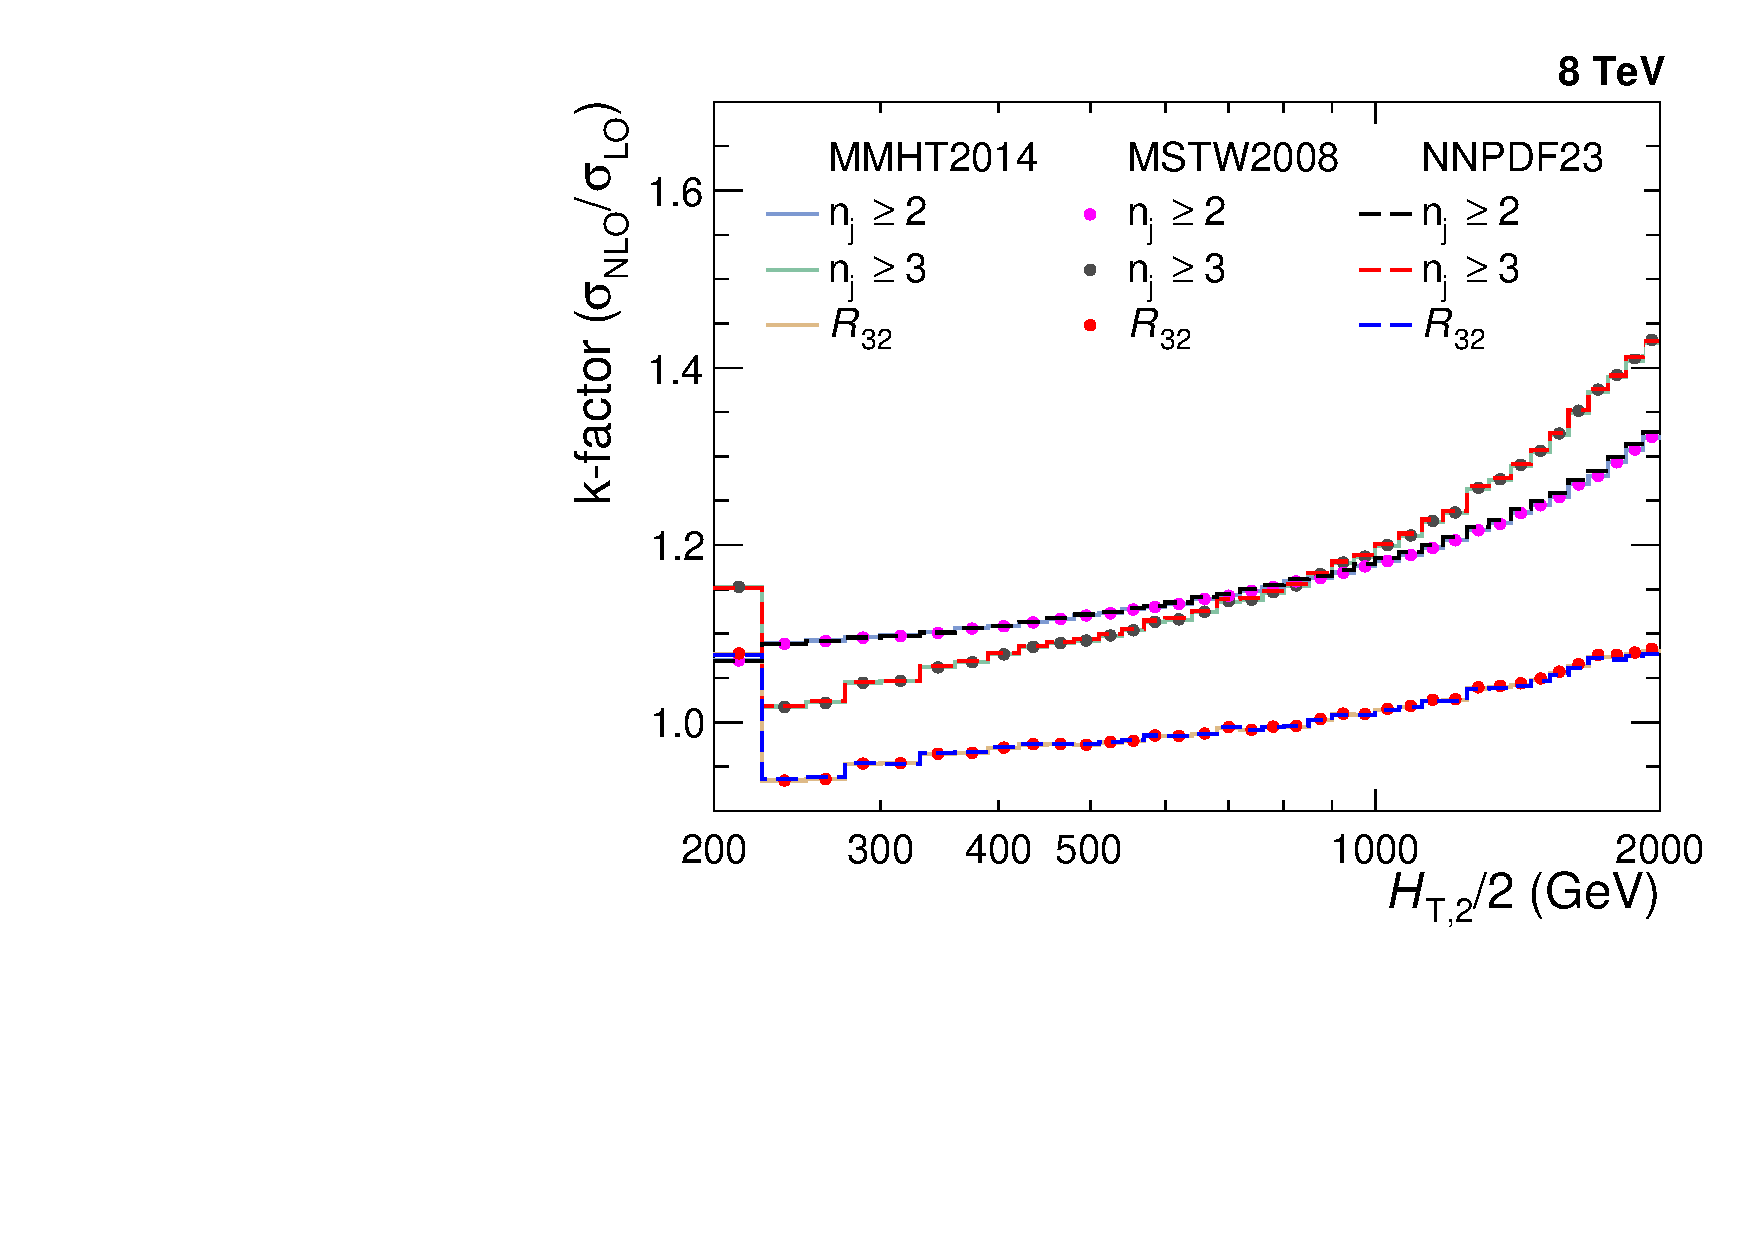
\includegraphics[scale = 0.24]{Plots_HT_2_150/Kfactor_all_2.pdf}\\
\end{frame}

%##################################### Slide : 36 ###########################################
\begin{frame}
\frametitle{\centerline{Details on PDF sets}}
\setlength\labelsep {\dimexpr\labelsep + 0.05em\relax}
\setlength\leftmarginiii{\dimexpr\leftmarginiii + 0.05em\relax}
\vspace{-4mm}
\begin{center}
\begin{itemize}
\item {\scriptsize Investigated PDF sets available via LHAPDF6 \\}
\end{itemize}
\vspace{-1.5mm}
\hspace{74mm}
\vspace{-4.mm}
\begin{table}[htbp]
  \centering\tiny
  \begin{tabular}{llclllc}
    \hline\hline
    Base set & N$_{F}$ & $M_t$ (GeV) &
    $M_Z$ (GeV) &\alpsmz & \alpsmz range\\ \hline
    % LHC Run 1
    ABM11     &    ~~5   & 180       & 91.174 & $0.1180$ & 0.110--0.130\\
    CT10      & ${\leq}5$ & 172       & 91.188 & $0.1180^*$ & 0.112--0.127\\
    MSTW2008  & ${\leq}5$ & ~$10^{10}$ & 91.1876 & $0.1202$ & 0.110--0.130\\
    NNPDF2.3  & ${\leq}6$ & 175       & 91.1876 & $0.1180^*$ & 0.114--0.124\\\hline\rbtrr\rbtrr
    % LHC Run 2
    CT14      & ${\leq}5$ & 172       & 91.1876 & $0.1180^*$ & 0.113--0.123\\
    HERAPDF2.0& ${\leq}5$ & 173       & 91.1876 & $0.1180^*$ & 0.110--0.130\\
    MMHT2014  & ${\leq}5$ & ~$10^{10}$ & 91.1876 & $0.1180^*$ & 0.108--0.128\\
    NNPDF3.0  & ${\leq}5$ & 173       & 91.2 & $0.1180^*$ & 0.115--0.121\\
    \hline\hline
  \end{tabular}
\end{table}
\vspace{-2mm}
{\tiny A * behind the \alpsmz values signifies that the parameter was fixed, not fitted \\}
%\begin{table}[p]
%  \centering \tiny
%  \begin{tabular}{lcccccc}
%    \hline\hline
%    \multirow{2}{*}{PDF set} & describes & pre-LHC/ & $\sigma$: \chisq &
%    \ratio: \chisq & PDF unc. & \multirow{2}{*}{\alpsmz}\\
%    & jet data & no jets & fit method &
%    fit method & @ each \alpsmz \\\hline
%    CT10       & \checkmark & \checkmark  & OK & OK &    ---     & 0.1180* \\
%    CT14       & \checkmark & ATLAS/CMS   & OK & OK &    ---     & 0.1180* \\
%    MSTW2008   & \checkmark & \checkmark  & OK & OK &    ---     & 0.1202  \\
%    MMHT2014   & \checkmark & ATLAS/CMS   & OK & OK &    ---     & 0.1180* \\
%    NNPDF2.3   & \checkmark & ATLAS       &  ? & OK & \checkmark & 0.1180* \\
%    ABM11      &     ---    & \checkmark  & OK & OK &    ---     & 0.1180  \\
%    \hline\hline
%  \end{tabular}
%\end{table}
\vspace{0.5mm}
\begin{itemize}
\item {\scriptsize Out of these eight PDF sets the following three will not be considered further :\\}
\tri
\begin{itemize}
\item {\scriptsize ABM11 : do not describe LHC jet data at small jet rapidity.
\vspace{1mm}
\item HERAPDF2.0 : exclusively fits HERA DIS data with only weak constraints on the gluon PDF.
\vspace{1mm}
\item NNPDF3.0 : the range in values available for \alpsmz is too limited. \\}
\end{itemize}
\vspace{1mm}
\ball
%\item \green{MSTW2008, MMHT2014 : 10$^{10}$ $\rightarrow$ Five flavours, with top quark mass $\approx$ infinity} \\} 
\end{itemize}
\end{center}
\end{frame}

%##################################### Slide : 37 ###########################################
\begin{frame}
\frametitle{\centerline{Non-Perturbative (NP) Corrections}}
\setlength\labelsep {\dimexpr\labelsep + 0.05em\relax}
\setlength\leftmarginiii{\dimexpr\leftmarginiii + 0.05em\relax}
\vspace{-2mm}
\begin{itemize}
\item {\scriptsize NP corrections are required to the NLO spectrum, to compare with the experimental measurements. \\}
\tri
\begin{itemize}
\item {\scriptsize {\bf PS correction :} partons emitted close to each other in phase space are not handled well in LO perturbation theories.
\vspace{0.5mm}
\item {\bf MPI and HAD :} cannot be modelled well within the perturbative framework.
\vspace{0.5mm}
\item LO generators : \mycolor{\PYTHIAS \Ztwostar, \HERWIGPP (tune 2.3)} 
\vspace{0.5mm}
\item NLO generator : \mycolor{\POWHEG \plusn \PYTHIAE~CUETS1}\\}
\end{itemize}
\ball
\vspace{-1.mm}
\item {\scriptsize NP correction factor is defined as \blue{$\rm \frac{\sigma^{PS\plusn HAD\plusn MPI}}{\sigma^{PS}}$}
\vspace{0.3mm}
\item Mean of the envelope gives the NP correction factor and the envelope covering all differences taken as uncertainty. \\}
\vspace{0.2mm}
%\item For \ratio : first the ratio of cross-sections of inclusive 3-jet to that of 2-jet events are taken seperately for hadronization and MPI effects switched off and on. Then the ratio defined above is used to calculate the NP correction factor. \\}
\end{itemize}
\vspace{-1.5mm}
%\begin{align*}
%\resizebox{.25\hsize}{!}{$\rm c^{NP}_{\ratio} = \frac{\Big(\frac{\sigma_{3\mbox{-}jet}}{\sigma_{2\mbox{-}jet}}\Big)^{PS\texttt{+}HAD\texttt{+}MPI}}{\Big(\frac{\sigma_{3\mbox{-}jet}}{\sigma_{2\mbox{-}jet}}\Big)^{PS}}$}
%\end{align*}
\vspace{1.mm}
%\begin{center}
\hspace{-3.5mm}
\begin{overpic}[scale=0.21]{Plots_HT_2_150/Final_NP_Corr_2.pdf}
\put(20,60){\mycolor{\bf {\scriptsize 2-jet}}}
\end{overpic}%
\begin{overpic}[scale=0.21]{Plots_HT_2_150/Final_NP_Corr_3.pdf}
\put(20,60){\mycolor{\bf {\scriptsize 3-jet}}}
\end{overpic}% 
\begin{overpic}[scale=0.21]{Plots_HT_2_150/Final_NP_Corr_Ratio_32.pdf}
\put(20,60){\mycolor{\bf {\scriptsize R$_{32}$}}}
\end{overpic}\\
%\end{center}
%\begin{itemize}
%\item {\scriptsize \blue{\bf NP effects get reduced in \rations.}\\}
%\end{itemize}
\end{frame}

%##################################### Slide : 38 ###########################################
\begin{frame}
\frametitle{\centerline{Electroweak Corrections (EW)}}
\setlength\labelsep {\dimexpr\labelsep + 0.05em\relax}
\setlength\leftmarginiii{\dimexpr\leftmarginiii + 0.05em\relax}
\begin{minipage}[tbp]{0.65\textwidth}
\begin{itemize}
 \item {\scriptsize At LHC, the center-of-mass energy of proton-proton collisions is well beyond EW scale $\sim{\cal O}$(100 GeV). 
 \item At such a high energy, the impact of higher order EW corrections is not any more negligible with respect to QCD effects.
\item Contributions from virtual exchanges of massive $W$ and $Z$ bosons.
\item \mycolor{Only available for inclusive 2-jet.}\\}
\end{itemize}
\end{minipage}
\begin{minipage}[tbp]{0.34\textwidth}
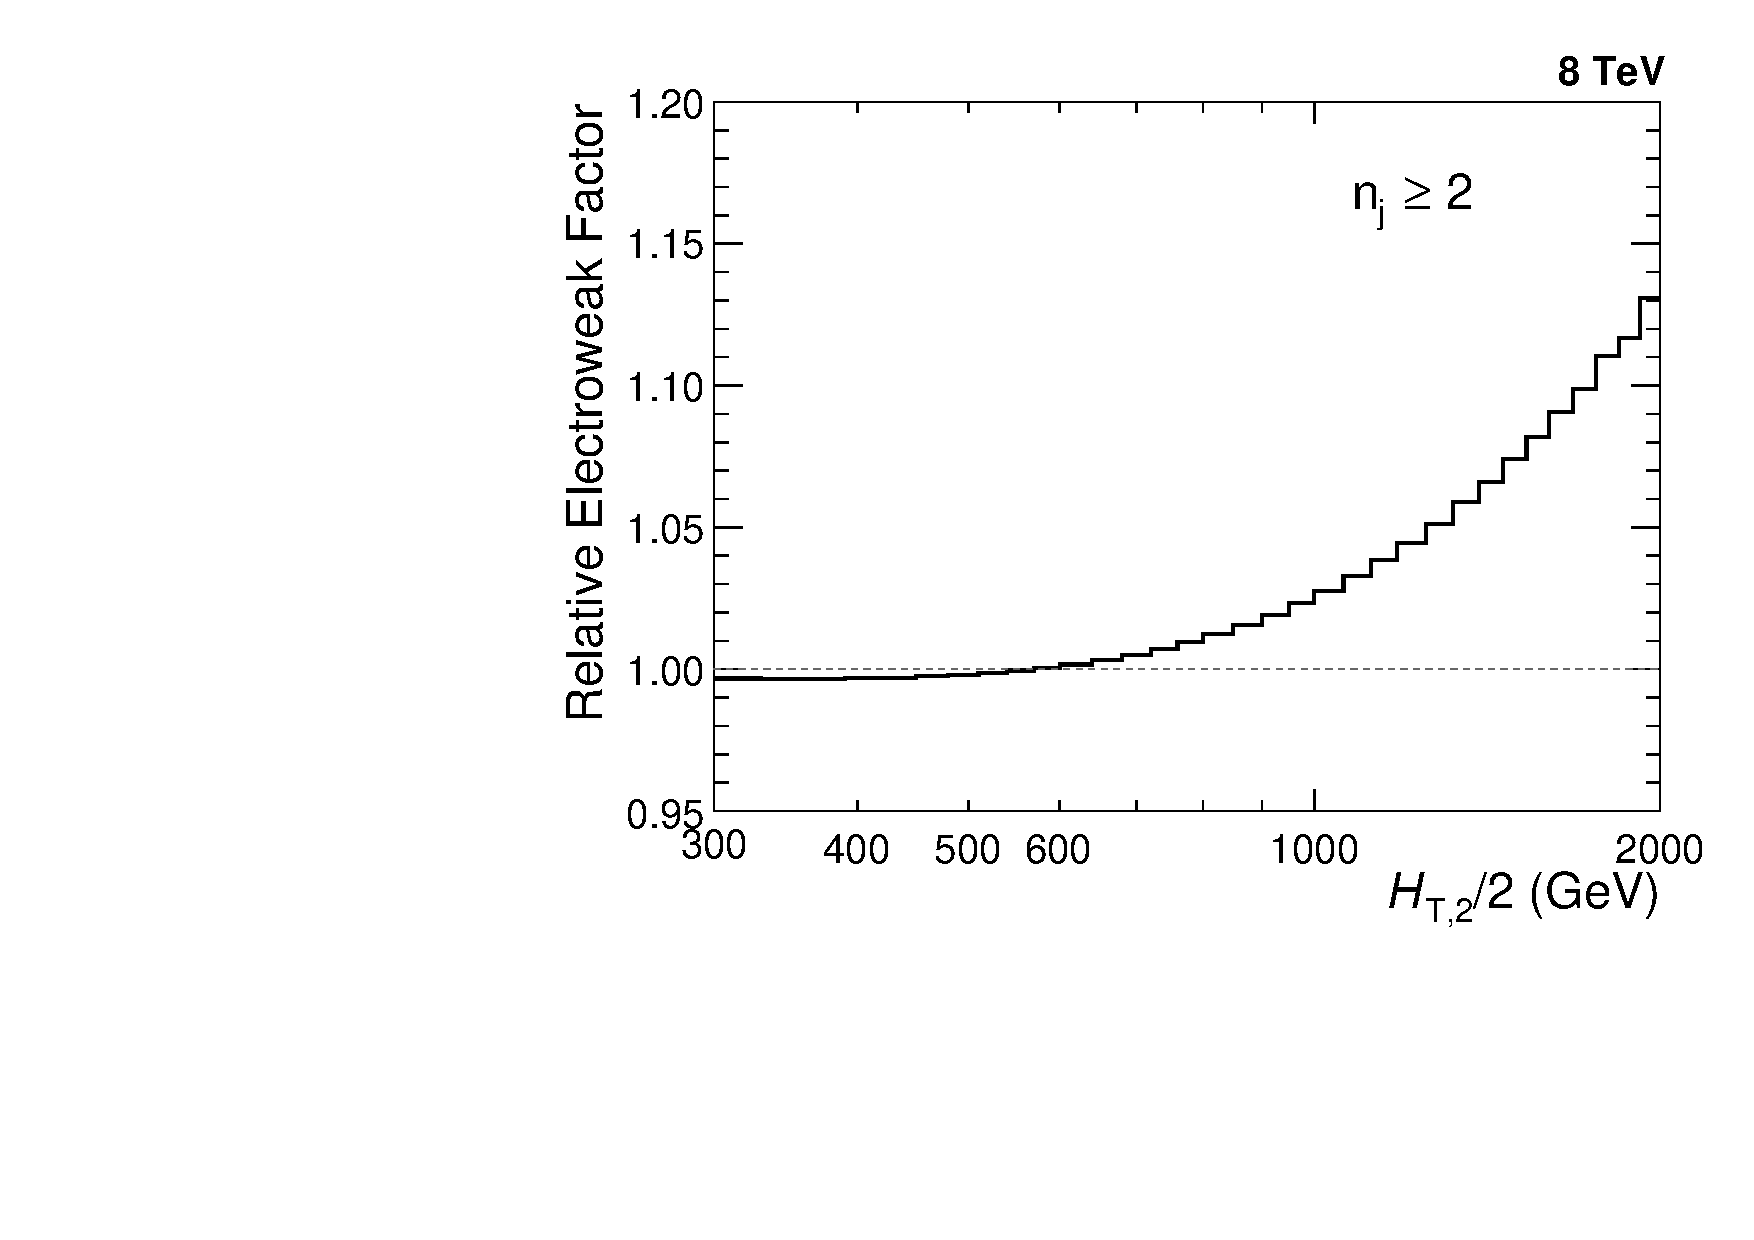
\includegraphics[scale=0.22]{Plots_HT_2_150/EW_2.pdf}%
\end{minipage}\\
\vspace{-1mm}
\begin{itemize}
\item {\scriptsize EW corrections explain the increasing systematic excess of data with respect to theory beyond 1 TeV of \httwotns.\\}
\end{itemize}
\vspace{0.5mm}
\begin{center}
\begin{overpic}[scale=0.24]{Plots_HT_2_150/Comparison_data_NLO_2_NoEW.pdf}
\put(40,75){\mycolor{\bf \scriptsize Without EW}}
\end{overpic}%
~~~~
\begin{overpic}[scale=0.24]{Plots_HT_2_150/Comparison_data_NLO_2_EW.pdf}
\put(40,75){\mycolor{\bf \scriptsize With EW}}
\end{overpic}
\end{center}
\end{frame}

%##################################### Slide : 39 ###########################################
\begin{frame}
\frametitle{\centerline{Theoretical Uncertainties}}
\setlength\labelsep {\dimexpr\labelsep + 0.05em\relax}
\setlength\leftmarginiii{\dimexpr\leftmarginiii + 0.05em\relax}
\vspace{-1mm}
\begin{center}
\begin{overpic}[scale = 0.25]{Plots_HT_2_150/Theory_Unc_2.pdf}
\put(20,15){\mycolor{\bf {\scriptsize 2-jet}}}
\end{overpic}%
\hspace{4mm}
\begin{overpic}[scale = 0.25]{Plots_HT_2_150/Theory_Unc_3.pdf}
\put(20,15){\mycolor{\bf {\scriptsize 3-jet}}}
\end{overpic} \\
\end{center}
\vspace{-3mm}
\begin{minipage}[tbp]{0.4\textwidth}
\vspace{-6mm}
\begin{table}[t]
  \tiny
   %\begin{tabular}{cccc}
   \begin{tabular}{ >{\arraybackslash}m{0.6in} >{\arraybackslash}m{0.53in} >{\arraybackslash}m{0.53in} >{\arraybackslash}m{0.55in} }
    \hline\hline
     Uncertainty Source & {\bf Inclusive 2-jet} & {\bf Inclusive 3-jet} & {\bf \ratio}\\\hline\rbtrr
     {\bf \mycolor{Scale}} & 5 to 13\% & 11 to 17\% & 6 to 8\% \\
     {\bf \green{PDF}} & 2 to 30\% & 2 to 30\% & 2 to 7\% \\
     {\bf \textcolor{lightskyblue}{NP}} & 1\% & 1 to 2\% & \ls 1\% \\\hline
     Total & 3 to 30\%             & 5 to 34\%             & 3 to 11\% \rbtrr\\
     \hline\hline
  \end{tabular}
\end{table}
\vspace{-3mm}
%\begin{itemize}
%\item \tiny {\green {Small dips at 1.X TeV in the PDF uncertainty (top right) : It is a feature of the CT10 PDF. Likewise the smaller dip at 700 GeV. If another PDF, e.g. CT14, is used, these dips are gone (Slide No.~\ref{theory_unc} in Back-Up). } \\}
%\end{itemize}
\end{minipage}
\hspace{23mm}
\begin{minipage}[tbp]{0.25\textwidth}
\vspace{1mm}
\begin{overpic}[scale = 0.25]{Plots_HT_2_150/Theory_Unc_Ratio_32.pdf}
\put(20,15){\mycolor{\bf {\scriptsize R$_{32}$}}}
\end{overpic}\\
\end{minipage}
\end{frame}
\ball

%##################################### Slide : 40 ###########################################
\begin{frame}
\begin{center}
\vspace{13mm}
\textbf{\Large\mycolor{Comparison of Data to Theory}}
\end{center}
\end{frame}

%##################################### Slide : 41 ###########################################
\begin{frame}
\frametitle{\centerline{Inclusive Differential Multijet Cross-Sections}}
\setlength\labelsep {\dimexpr\labelsep + 0.05em\relax}
\setlength\leftmargini{\dimexpr\leftmargini + 0.05em\relax}
\begin{minipage}[tbp]{0.6\textwidth}
\begin{itemize}
\item {\scriptsize \NLOJETPP predictions based on the CT10 PDF set and corrected for NP effects, in addition for EW effects in the 2-jet case :\\}
\tri
\begin{itemize}
\item {\scriptsize Compatible with data within uncertainties over a wide range of \httwot from 300 GeV up to 2 TeV. \\}
\end{itemize}
\ball
\item {\scriptsize Predictions from \MGP, corrected for EW effects in the 2-jet case : \\}
\tri
\begin{itemize}
\item {\scriptsize significant discrepancies are visible in the ratio for comparison with the leading-order (LO) tree-level prediction. \\}
\end{itemize}
\end{itemize}
\vspace{-6mm}
\begin{center}
\begin{overpic}[scale = 0.24]{Plots_HT_2_150/Sensitivity_ratio_32_CT10_only.pdf}
\put(20,60){\mycolor{\bf {\scriptsize R$_{32}$}}}
\end{overpic}
\end{center}
\end{minipage}
\begin{minipage}[tbp]{0.3\textwidth}
\begin{overpic}[scale = 0.24]{Plots_HT_2_150/Comparison_data_theory_EW.pdf}
\put(52,42){\mycolor{\bf {\scriptsize 2-jet}}}
\put(40,25){\green{\bf {\scriptsize 3-jet}}}
\end{overpic}\\
\vspace{1mm}
\begin{overpic}[scale = 0.24]{Plots_HT_2_150/Comparison_data_MC_EW.pdf}
\put(52,42){\textcolor{lightskyblue}{\bf {\scriptsize 2-jet}}}
\put(40,25){\textcolor{pink}{\bf {\scriptsize 3-jet}}}
\end{overpic}%
\end{minipage}
\end{frame}
\ball

%##################################### Slide : 42 ###########################################
\begin{frame}
\frametitle{\centerline{Data-Theory Comparison}}
\setlength\labelsep {\dimexpr\labelsep + 0.05em\relax}
\setlength\leftmargini{\dimexpr\leftmargini + 0.05em\relax}
\vspace{-2.2mm}
\begin{itemize}
\item {\scriptsize Ratios to NLO$\otimes$NP$\otimes$EW - CT10\\}
\end{itemize}
\hspace{-5.3mm}
\begin{overpic}[scale = 0.215]{Plots_HT_2_150/Comparison_data_NLO_Pdfs_2_EW.pdf}
\put(20,60){\mycolor{\bf {\scriptsize 2-jet}}}
\end{overpic}%
\begin{overpic}[scale = 0.215]{Plots_HT_2_150/Comparison_data_NLO_Pdfs_3.pdf}
\put(20,60){\mycolor{\bf {\scriptsize 3-jet}}}
\end{overpic}%
\begin{overpic}[scale = 0.215]{Plots_HT_2_150/Comparison_data_NLO_Pdfs_ratio_32.pdf}
\put(20,60){\mycolor{\bf {\scriptsize R$_{32}$}}}
\end{overpic}
\vspace{-5mm}
\begin{itemize}
\item {\scriptsize Ratios to \POWHEG \plusn \PYTHIAE~tune CUETS1\\}
\item[] {\scriptsize - \blue{\POWHEG \plusn \PYTHIAE~with tune CUETM1} better describes the 2-jet event cross-section, but fails for the 3-jet case.\\}
\end{itemize}
\hspace{-5.3mm}
\begin{overpic}[scale = 0.215]{Plots_HT_2_150/Comparison_data_MC_samples_2_Pow_EW.pdf}
\put(75,60){\mycolor{\bf {\scriptsize 2-jet}}}
\end{overpic}%
\begin{overpic}[scale = 0.215]{Plots_HT_2_150/Comparison_data_MC_samples_3_Pow.pdf}
\put(75,60){\mycolor{\bf {\scriptsize 3-jet}}}
\end{overpic}%
\begin{overpic}[scale = 0.215]{Plots_HT_2_150/Comparison_data_MC_samples_ratio_32_Pow.pdf}
\put(75,60){\mycolor{\bf {\scriptsize R$_{32}$}}}
\end{overpic}
\end{frame}

%##################################### Slide : 43 ###########################################
\begin{frame}
\begin{center}
\vspace{13mm}
\textbf{\Large\mycolor{Determination of the Strong Coupling Constant}}
\end{center}
\end{frame}

%##################################### Slide : 44 ###########################################
\begin{frame}
\frametitle{\centerline{Determination of the Strong Coupling Constant}}
\setlength\labelsep {\dimexpr\labelsep + 0.05em\relax}
\setlength\leftmargini{\dimexpr\leftmargini + 0.05em\relax}
\begin{itemize}
\vspace{-2mm}
\item {\scriptsize Differential inclusive jet production cross-section up to NLO :
\begin{align*}
\blue{\frac{d\sigma}{d(\httwotns)} = \alpha_S^2(\mur)\hat{X}^{(0)}(\muf,\httwotns)\big[1~\plus \alpha_S(\mur)K1(\mur, \muf,\httwotns)\big]}
 \end{align*}
\item \alpsmz is determined by minimizing the \chisq between the measurements and the theoretical predictions : \\}
\end{itemize}
\vspace{-3mm}
\begin{align*}
\blue{\resizebox{.38\hsize}{!}{$\chsq = M^{T}C^{-1}M,~~~M^{i}= D^{i}-T^{i}$}}
\end{align*}
\vspace{-5mm}
\begin{itemize}
\item {\scriptsize $C =\rm{C_{exp} + C_{theo}}$ is the sum of covariances of experimental and theoretical sources of uncertainty as follows : \\}
\end{itemize}
\vspace{-3mm}
\begin{center}
%\begin{align*} 
\blue{\resizebox{.8\hsize}{!}{$\rm C_\mathrm{exp} = \mathrm{Cov}^\mathrm{ExpStat} ~\plus~ \sum\mathrm{Cov}^\mathrm{JEC} ~\plus~
  \mathrm{Cov}^\mathrm{Unfolding} ~\plus~
  % \mathrm{Cov}^\mathrm{JER} ~\plus~
  \mathrm{Cov}^\mathrm{Lumi} ~\plus~
  \mathrm{Cov}^\mathrm{Uncor}$}\\
  \vspace{0mm}
  \resizebox{.42\hsize}{!}{$\rm C_\mathrm{theo} = \mathrm{Cov}^\mathrm{TheoStat} ~\plus~ \mathrm{Cov}^\mathrm{NP} ~\plus~ \mathrm{Cov}^\mathrm{PDF}$}}
 % \end{align*}
  \end{center}
\vspace{-2.5mm}  
  \tri
\begin{itemize}
\item[]
\begin{itemize}
\item{\tiny {$\mathrm{Cov}^\mathrm{ExpStat}$: the statistical uncertainty of the data including correlations introduced by the unfolding,}
\item{$\mathrm{Cov}^\mathrm{JEC}$: the JEC
systematic uncertainty,}
\item{$\mathrm{Cov}^\mathrm{Unfolding}$: the unfolding systematic uncertainty including the JER,}
\item{$\mathrm{Cov}^\mathrm{Lumi}$: the luminosity uncertainty,}
\item{$\mathrm{Cov}^\mathrm{Uncor}$: a residual uncorrelated systematic uncertainty summarizing individual causes such as trigger and identification inefficiencies, time dependence of the jet \pt resolution, and uncertainty on the trigger prescale factors,}
\item{$\mathrm{Cov}^\mathrm{TheoStat}$: the statistical uncertainty caused by numerical integrations in the cross-section computations,}
\item{$\mathrm{Cov}^\mathrm{NP}$: the systematic uncertainty of the NP corrections, and}
\item{$\mathrm{Cov}^\mathrm{PDF}$: the PDF uncertainty.} \\}
\end{itemize}
\vspace{1mm}
\ball
\item {\scriptsize \mycolor{300 \ls \httwot \ls 1000 GeV} for the fits of the cross-sections : to avoid the region close to the minimal \pt~threshold of 150 GeV for each jet at low \pt~and the onset of electroweak effects at high \pt.\\}
\end{itemize}
\end{frame}

%##################################### Slide : 45 ###########################################
\begin{frame}
\frametitle{\centerline{Fit results in range 300 \ls \httwot \ls 1000 GeV}}
\setlength\labelsep {\dimexpr\labelsep + 0.05em\relax}
\setlength\leftmargini{\dimexpr\leftmargini + 0.05em\relax}
%\vspace{-3.4mm}
\begin{center}
%\vspace{-0.4mm}
%\vspace{-2mm}
\begin{table}[htbp]
  \centering\scriptsize
\begin{tabular}{l|ccc|ccc}
    \hline\hline
    \multirow{2}{*}{PDF set} & \multicolumn{3}{c|}{Inclusive 2-jets} & \multicolumn{3}{c}{Inclusive 3-jets} \\
    & \alpsmz & $\pm\Delta\alpsmz$ & \chisqndof &\alpsmz & $\pm\Delta\alpsmz$ & \chisqndof \\\hline\rbtrr
    % ABM11          & 0.1240 & 0.0025 & 11./18 & 0.1241 & 0.0020 & 10./18 \\
    CT10           & 0.1174 & 0.0032 & 3.0/18 & 0.1169 & 0.0027 & 5.4/18 \\
    CT14           & 0.1160 & 0.0035 & 3.5/18 & 0.1159 & 0.0031 & 6.1/18 \\
    MSTW2008       & 0.1159 & 0.0025 & 5.3/18 & 0.1161 & 0.0021 & 6.7/18 \\
    MMHT2014       & 0.1165 & 0.0034 & 5.9/18 & 0.1166 & 0.0025 & 7.1/18 \\
    NNPDF2.3       & 0.1183 & 0.0025 & 9.7/18 & 0.1179 & 0.0021 & 9.1/18 \\

    \hline\hline
    \end{tabular}
\end{table}
\vspace{1mm}
\begin{table}[htbp]
  \centering\scriptsize
  \begin{tabular}{l|ccc|ccc}
    \hline\hline
    \multirow{2}{*}{PDF set} & \multicolumn{3}{c|}{2- \& 3-jets ({\bf Ignored correlations})} & \multicolumn{3}{c}{\ratio ({\bf Accounted for correlations})} \\
    & \alpsmz & $\pm\Delta\alpsmz$ & \chisqndof &\alpsmz & $\pm\Delta\alpsmz$ & \chisqndof \\\hline\rbtrr
    CT10           & 0.1170 & 0.0026 & 8.2/37 & 0.1141 & 0.0028 & 19./18 \\
    CT14           & 0.1161 & 0.0029 & 9.1/37 & 0.1139 & 0.0032 & 15./18 \\
    MSTW2008       & 0.1161 & 0.0021 & 11./37 & 0.1150 & 0.0023 & 21./18 \\
    MMHT2014       & 0.1168 & 0.0025 & 11./37 & 0.1142 & 0.0022 & 19./18 \\
    NNPDF2.3       & 0.1188 & 0.0019 & 15./37 & 0.1184 & 0.0021 & 12./18 \\
    \hline\hline
  \end{tabular}
\end{table}
\vspace{1mm}
\begin{itemize}
\item {\scriptsize All cross-section fits give compatible values for \alpsmz in the range of 0.115~-~0.118.
\vspace{1mm}
\item For \rations, smaller values are obtained.
\vspace{1mm}
\item Small \chisqndof~except for the \ratio fits : may be due to an overestimation of the residual uncorrelated uncertainty of 1\% that is cancelled for \rations.\\} 
\vspace{1mm}
%\item With an assumed uncertainty of 0.25\% : the \chisqndof~values lie around unity while the \alpsmz values are still compatible with the previous results but with slightly reduced uncertainties. \\}
\end{itemize}
\end{center}
\end{frame}

%##################################### Slide : 46 ###########################################
\begin{frame}
\frametitle{\centerline{Fit results in range 300 \ls \httwot \ls 1680 GeV}}
\setlength\labelsep {\dimexpr\labelsep + 0.05em\relax}
\setlength\leftmargini{\dimexpr\leftmargini + 0.05em\relax}
\begin{center}
\vspace{-3mm}
\begin{itemize}
\item {\scriptsize \alpsmz fits to the 2-jet event cross-section with or without EW correction factors. \\}
\tri 
\begin{itemize}
\item {\scriptsize Reduction in \chisqndof~indicating a better agreement when EW effects are included. 
\vspace{1mm}
\item A tendency to slightly smaller \alpsmz values is observed without the EW corrections. \\}
\end{itemize}
\ball
\end{itemize}
\vspace{-1mm}
\begin{table}[p]
   \centering\tiny
  \begin{tabular}{l|ccc|ccc}
    \hline\hline
    \multirow{2}{*}{PDF set} & \multicolumn{3}{c|}{2-jets, without EW} &
    \multicolumn{3}{c}{2-jets, with EW} \\
    & \alpsmz & $\pm\Delta\alpsmz$ & \chisqndof &\alpsmz & $\pm\Delta\alpsmz$ & \chisqndof \\\hline
    CT10           & 0.1163 & 0.0034 & 15./28 & 0.1165 & 0.0032 & 14./28 \rbtrr\\
    CT14           & 0.1137 & 0.0033 & 24./28 & 0.1144 & 0.0033 & 17./28 \rbtrr\\
    MSTW2008       & 0.1093 & 0.0028 & 27./28 & 0.1133 & 0.0023 & 19./28 \rbtrr\\
    MMHT2014       & 0.1127 & 0.0032 & 32./28 & 0.1141 & 0.0032 & 21./28 \rbtrr\\
    NNPDF2.3       & 0.1162 & 0.0024 & 31./28 & 0.1168 & 0.0024 & 23./28 \rbtrr\\
    \hline\hline
  \end{tabular}
\end{table}

\begin{itemize}
\item {\scriptsize Results from the two most compatible PDF sets \mycolor{MSTW2008} and \mycolor{MMHT2014} at NLO : \\}
\tri 
\begin{itemize}
\item {\scriptsize Provide a large enough range in \alpsmz values to ensure fits without extrapolation.
\vspace{0.7mm}
\item Other three PDF sets are at the limit such that reliable fits cannot be performed for estimation of all uncertainties. 
\vspace{0.7mm}
\item \mycolor{Scale uncertainty} is the most dominant source of total uncertainty on \alpsmzns. \\}
\end{itemize}
\ball 
\end{itemize}
\vspace{-1mm}
\begin{table}[p]
   \centering\scriptsize
  \begin{tabular}{l|ccccccc}
    \hline\hline
    \multirow{2}{*}{PDF set} & & \multicolumn{5}{c}{\ratio: $\Delta\alpsmz\times1000$} & \\
    & \alpsmz & exp & PDF & NP & all exc.\ scale & scale & \chisqndof \\\hline\rbtrr
    MSTW2008  & 0.1150 & $\pm10$ & $\pm13$ & $\pm15$ & $\pm23$ & $^{+50}_{-0}$ & 26./28 \\
    MMHT2014  & 0.1142 & $\pm10$ & $\pm13$ & $\pm14$ & $\pm22$ & $^{+49}_{-6}$ & 24./28 \\
    \hline\hline
  \end{tabular}
\end{table}
\end{center}
\end{frame}

%##################################### Slide : 47 ###########################################
\begin{frame}
\frametitle{\centerline{Running of the Strong Coupling Constant}}
\setlength\labelsep {\dimexpr\labelsep + 0.05em\relax}
\setlength\leftmargini{\dimexpr\leftmargini + 0.05em\relax}
\begin{center}
\begin{itemize}
\item {\scriptsize \alps depends on the energy scale $Q$; decreases with the increase of scale $Q$.
\begin{align*}
\blue{Q_{j} = \frac[10pt]{\sum\limits_{i=1}^{N^{j}_{bin}} H^{i}_{\rm T,2} \bigg[{\dd{\sigma}{(\httwotns)}}\bigg]^{i}}{\sum\limits_{i=1}^{N^{j}_{bin}} \bigg[{\dd{\sigma}{(\httwotns)}}\bigg]^{i}}}
\end{align*}
%\item Value of \alpsmz is extracted in each \httwot range. 
\item Extracted \alpsmz in ranges of \httwot $\rightarrow$ evolved to \alpsq.
\vspace{1mm}
\item Evolution is performed for five flavors at 2-loop order with the \RunDec program.\\}
\end{itemize}
\begin{table}[htbp]
\centering\scriptsize
\vspace{2mm}
\begin{tabular}{cccccc}
   \hline\hline\rbtrrn
    \httwot & $\langle{}Q\rangle$ & \alpsmz & \alpsq & No.\ of data & \chisqndof\\
    (GeV) & (GeV) & & & points & \rbtrr\\\hline
    % v4
    300 - 420 \rbtrr  &  340 &
    $0.1157\,^{+0.0060}_{-0.0030}$ & $0.0969\,^{+0.0041}_{-0.0021}$ &  4 & 2.8/3 \rbthm\\
    420 - 600 \rbtrr  &  476 &
    $0.1153\,^{+0.0062}_{-0.0025}$ & $0.0928\,^{+0.0039}_{-0.0016}$ &  6 & 6.1/5 \rbthm\\
    600 - 1000\rbtrr  &  685 &
    $0.1134\,^{+0.0059}_{-0.0028}$ & $0.0879\,^{+0.0035}_{-0.0017}$ &  9 & 7.1/8 \rbthm\\
    1000 - 1680\rbtrr & 1114 &
    $0.1147\,^{+0.0074}_{-0.0040}$ & $0.0841\,^{+0.0039}_{-0.0021}$ & 10 & 5.4/9 \rbthm\\
    \hline\hline
  \end{tabular}
\end{table}
\end{center}
\end{frame}

%##################################### Slide : 48 ###########################################
\begin{frame}
\frametitle{\centerline{Running of the Strong Coupling Constant}}
\setlength\labelsep {\dimexpr\labelsep + 0.05em\relax}
\setlength\leftmargini{\dimexpr\leftmargini + 0.05em\relax}
\vspace{1mm}
\begin{center}
\begin{overpic}[scale=0.55]{Plots_HT_2_150/Running_alphas_8TeV_R32_2_edited.pdf}
\put(68,28){\textcolor{red!75!black}{\bf R$_{32}$ ($\sqrt{s}$ = 8 TeV)}}
\end{overpic}
\end{center}
\end{frame}

%##################################### Slide : 49 ###########################################
\begin{frame}
\frametitle{\centerline{Summary-I~}}
\setlength\labelsep {\dimexpr\labelsep + 0.05em\relax}
\setlength\leftmarginiii{\dimexpr\leftmarginiii + 0.05em\relax}
\vspace{-3.5mm}
\begin{center}
\begin{itemize}
\item {\footnotesize Inclusive multijet production cross-section measured precisely in terms of jet transverse momentum is one of the important observables in understanding physics at hadron colliders.
\vspace{0.5mm}
\item The inclusive 2-jet (3-jet) event cross-sections have been measured as a function of the average \pt~of the two leading jets (\httwotns) in a range of 0.3 \ls \httwot \ls 2.0 TeV (0.3 \ls \httwot \ls 1.68 TeV).
\vspace{0.5mm}
\item Cross-section ratio \ratio is obtained by dividing the differential cross-sections of inclusive 3-jet events to that of inclusive 2-jet one in each bin of \httwotns. 
\vspace{0.5mm}
\item LO tree-level MC predictions obtained using \MadGraphF \plusn \PYTHIAS exhibit significant deviations.
\vspace{0.5mm}
\item Measurements, after correcting for detector effects by using an iterative unfolding procedure, are well described by NLO calculations, complemented with NP corrections important at low \httwotns. 
\item Upwards trend observed in 2-jet data at high \httwot is explained by the onset of electroweak (EW) corrections.\\}
\end{itemize}
\end{center}
\end{frame}

%##################################### Slide : 50 ###########################################
\begin{frame}
\frametitle{\centerline{Summary-II}}
\setlength\labelsep {\dimexpr\labelsep + 0.05em\relax}
\setlength\leftmarginiii{\dimexpr\leftmarginiii + 0.05em\relax}
\vspace{-3.5mm}
\begin{center}
\begin{itemize}
\item {\footnotesize \alps Determination : \\}
\tri
\begin{itemize}
\item {\footnotesize Inclusive multijet cross-sections, $\sigma_{\rm n\hy jet} \propto\alpha^{\rm n}_{\rm s}$ are used to extract the value of \alpsmzns. 
\vspace{0.5mm}
\item Cross-section is a better tool as many uncertainties and PDF dependencies largely cancel. 
\vspace{0.5mm}
\item Performed fits of \alpsmz from differential inclusive 2-jet and inclusive 3-jet event cross-sections separately and in combined fit as well as ratio \rations.
\vspace{0.5mm}
\item The strong coupling constant is determined in a fit to the \ratio measurement. \\}
\cir
\begin{itemize}
\item {\footnotesize {\bf Using MSTW2008 PDF set -} \\}
\vspace{1mm}
\blue{\bf \tiny $\alpsmz = 0.1150\,\pm0.0010\,\textrm{(exp)}\,\pm0.0013\,\textrm{(PDF)}\,\pm0.0015\,\textrm{(NP)}\,^{+0.0050}_{-0.0000}\,\textrm{(scale)}$ \\ \hspace*{9mm} = $0.1150\,\pm0.0023\,\textrm{(all except scale)}\,^{+0.0050}_{-0.0000}\,\textrm{(scale)}$ \\}
\vspace{1mm}
\item {\footnotesize Using {\bf MMHT2014 PDF} set - \\}
\vspace{1mm}
\blue{\bf \tiny $\alpsmz = 0.1142\,\pm0.0010\,\textrm{(exp)}\,\pm0.0013\,\textrm{(PDF)}\,\pm0.0014\,\textrm{(NP)}\,^{+0.0049}_{-0.0006}\,\textrm{(scale)}$ \\ \hspace*{9mm} = $0.1142\,\pm0.0022\,\textrm{(all except scale)}\,^{+0.0049}_{-0.0006}\,\textrm{(scale)}$\\} 
\end{itemize}
\tri
\item {\footnotesize Running of \alpsq~as a function of $Q$ is in well agreement within uncertainties with the world average value of \mycolor{\alpsmz = 0.1181 $\pm$ 0.0011}.\\}
\end{itemize}
\end{itemize}
\end{center}
\end{frame}
\ball

%##################################### Slide : 51 ###########################################
\begin{frame}
\frametitle{\centerline{Other Activities}}
\setlength\labelsep {\dimexpr\labelsep + 0.05em\relax}
\setlength\leftmarginiii{\dimexpr\leftmarginiii + 0.05em\relax}
\vspace{-1mm}
\begin{center}
\begin{itemize}
\item {\scriptsize LHC went under first long shutdown (LS1) in 2013-2014 for upgradation in which the the proton beam energy was increased from 4 TeV to 6.5 TeV per beam. \\}
\tri
\begin{itemize}
{\item \scriptsize Hybrid Photon Detectors (HPDs) of Outer Hadron calorimeter (HO) were replaced by Silicon Photomultipliers (SiPMs).
\vspace{0.8mm}
\item Participated in the {\bf re-installation of the readout modules (RMs) with SiPMs} in the sectors YB\plusn 1 and YB\plusn 2 of HCAL in March-April, 2014.
\vspace{0.8mm}
\item Studied the {\bf optimization} of SiPM operational variables.
\vspace{0.8mm}
\item VME based system was replaced with {\bf \mtca (Micro Telecommunications Computing Architecture)} standard system in HCAL back-end electronics.\\}
\cir
\begin{itemize}
{\item \scriptsize Power Mezzanines/Auxiliary Power Mezzanines (PMs/APMs) mounted on \mhtr cards supply power.
\item Power Mezzanine Testing program : a long term ($\sim$39 hour) stability test to monitor/test PMs/APMs.
\item {\bf Installed test-stand at Department of Physics, PU, Chandigarh.}\\}
\end{itemize}
\end{itemize}
\ball
\item {\scriptsize Worked in {\bf Data Certification (DC)} sub-group of the Data Quality Monitoring (DQM) group of Physics Performance \& Dataset (PPD) organization for performing the certification of 2016 CMS data.
\vspace{0.8mm}
\item Participated in software development of a tool called {\bf Historic DQM (HDQM)} which is beneficial to study and check stability of various sub-detectors with time.
\vspace{0.8mm}
\item Participated in CMS data taking as a {\bf DAQ shifter}.\\}
\end{itemize}
\vspace{-3.5mm}
\hspace*{80mm}\begin{beamercolorbox}[wd=28mm,ht=3.mm,center,shadow=true, rounded=true]{redgrey}
{}
{\scalebox {0.7} {\mycolor{\LARGE{\bf THANKS!!}}}}
\end{beamercolorbox}
\end{center}
\end{frame}

%##################################### Slide : ###########################################
\begin{frame}
\begin{center}
\vspace{13mm}
\textbf{\Large\mycolor{Back-up slides}}
\end{center}
\end{frame}

%##################################### Slide : ###########################################
\begin{frame}
\frametitle{\centerline{Sequential Recombination Algorithms}}
\setlength\labelsep {\dimexpr\labelsep + 0.05em\relax}
\setlength\leftmargini{\dimexpr\leftmargini + 0.05em\relax}
\begin{itemize}
\item {\scriptsize Based on transverse momentum \pt~of the particles.\\}
\begin{enumerate}
{\scriptsize \item Distance $d_{ij}$ between two particles $i$ and $j$ and distance $d_{iB}$ of the particle to the beam are calculated as\\
\begin{equation}
\begin{gathered}
d_{ij} = {\rm min}\big(p^{2p}_{{\rm T}i},p^{2p}_{{\rm T}j}\big) \frac{\Delta R^2_{ij}}{R^2}, ~~~~d_{iB} = p^{2p}_{{\rm T}i} \\ {\rm where} ~~~\Delta R^2_{ij} = (y_i -y_j)^{2} ~\plus (\phi_i -\phi_j)^{2}
\end{gathered}
\end{equation}
\item If $d_{ij}$ \ls $d_{iB}$, particles $i$ and $j$ are merged into a new single jet object $k$, summing four-momenta of two initial particles by recombination scheme and step 1 is repeated. 
\vspace{1mm} 
\item If $d_{iB}$ \ls $d_{ij}$, particle $i$ is declared as a final-state jet and the particle gets removed from the list.\\}
\end{enumerate}
\item {\scriptsize Value of the parameter $p$ defines the three different sequential algorithms :\\}
\tri
\begin{itemize}
\item {\scriptsize \kt algorithm : {\bf $p$ = 1}
\vspace{1mm} 
\item Cambridge/Aachen (C/A) algorithm : {\bf $p$ = 0} 
\vspace{1mm} 
\item anti-$k_{T}$ algorithm : {\bf $p$ = -1} \\}
\end{itemize}
\end{itemize}
\end{frame}

%##################################### Slide :  ###########################################
\begin{frame}
\frametitle{\centerline{Event Selection}}
\setlength\labelsep {\dimexpr\labelsep + 0.05em\relax}
\setlength\leftmargini{\dimexpr\leftmargini + 0.05em\relax}
\begin{center}
\begin{itemize}
 \item {\scriptsize anti-\kt particle flow (PF) jets with R = 0.7.
\vspace{2.0mm}
\item At least one good primary vertex : $|${z(PV)}$|$\ls 24 cm, $\rho$(PV) $<$ 2 cm, $ndof >$ 4
\vspace{2.0mm}
\item Official tight jet ID recommended by \JetMet group is used.
\vspace{1.0mm}
\begin{table}[!htbp]
 \centering\tiny
 \begin{tabular}{lll}
 \hline\hline
                      & {\bf Property}          & {\bf Tight ID cut} \rbthm\\\hline
                      & neutral hadron fraction & ~~~~~~\ls 0.90       \rbtrr \\
  Whole               & neutral EM fraction     & ~~~~~~\ls 0.90       \rbtrr \\
 $\eta$ region        & number of constituents  & ~~~~~~\gr 1          \rbtrr \\
                      & muon fraction           & ~~~~~~\ls 0.80       \rbtrr \\ \hline
                      & charged hadron fraction & ~~~~~~\gr 0          \rbtrr \\
only $|\eta|$ \ls 2.4 & charged multiplicity    & ~~~~~~\gr 0          \rbtrr \\
                      & charged EM fraction     & ~~~~~~\ls 0.90       \rbtrr \\                  
\hline\hline
 \end{tabular}
\end{table}
\vspace{1.0mm}
\item All jets having \pt \gr 150 GeV and $|y|$ \ls 5.0 are selected.
\vspace{2.0mm}
\item Events with at least two jets are selected.
\vspace{2.0mm}
\item The two leading jets should have $|y|$ \ls 2.5 and further jets are counted only, if they lie within the same central rapidity range of $|y|$ \ls 2.5.
\vspace{2.0mm}
\item ${\frac{\ETmiss}{\sum\ET}}$ $\textless$ 0.3 to protect against mismeasured or background events with large missing \ET.\\}
\end{itemize}
\end{center}
\end{frame}

%##################################### Slide :  ###########################################
\begin{frame}
\frametitle{\centerline{Datasets \& MC Samples}}
\setlength\labelsep {\dimexpr\labelsep + 0.05em\relax}
\setlength\leftmargini{\dimexpr\leftmargini + 0.05em\relax}
\vspace{-2mm}
\begin{center}
\begin{itemize}
\item {\scriptsize {\bf Data :} Collected at \cme~= 8 TeV during 2012 run; Integrated Luminosity : {\bf 19.7 \fbinv} \\}
\begin{table}[!h]
\centering\tiny
\hspace*{-6mm}\begin{tabular}{>{\centering\arraybackslash}m{0.25in}cl>{\centering\arraybackslash}m{0.97in}}
\hline\hline
{\bf Run} & {\bf Run range} & {\bf \hspace*{12mm}Data set}          & {\bf Luminosity (\fbinv)} \rbtrr\\\hline

   A       & 190456-193621   & /Jet/Run2012A-22Jan2013-v1/AOD         & 0.88  \rbtrr\\
   B       & 193834-196531   & /Jet[Mon,HT]/Run2012B-22Jan2013-v1/AOD & 4.41  \rbtrr\\
   C       & 198022-203742   & /Jet[Mon,HT]/Run2012C-22Jan2013-v1/AOD & 7.06  \rbtrr\\
   D       & 203777-208686   & /Jet[Mon,HT]/Run2012D-22Jan2013-v1/AOD & 7.37  \rbtrr\\
\hline\hline
\end{tabular}
\end{table}
\vspace{1mm}
%\tri
%\begin{itemize}
%\item {\scriptsize CMS software : CMSSW\_5\_3\_11
%\vspace{1mm}
%\item JECs : Winter14\_V8
%\vspace{1mm}
%\item Json file: Cert\_190456-208686\_8TeV\_22Jan2013ReReco\_Collisions12\_JSON.txt \\ }
%\end{itemize}
\ball
\vspace{1mm}
\item {\scriptsize {\bf Simulated Monte-Carlo (MC) Samples :} \\}
\vspace{-2mm} 
\begin{table}[!h]
\centering\tiny
\hspace*{-6mm}\begin{tabular}{lc>{\centering\arraybackslash}m{0.6in}c}

\hline\hline
{\bf Generator} & {\bf Sample} & {\bf Events} & {\bf Cross-section (pb)}\rbtrr\\\hline
 & \makecell{{\tiny /{\bf QCD\_HT-100To250}\_TuneZ2star\_8TeV-madgraph-pythia6/\vspace{0mm}}\\{\tiny Summer12\_DR53X-PU\_S10\_START53\_V7A-v1/AODSIM}} & 50129518 & 1.036 $\times$ 10$^7$ \rbtrr\\
 \makecell{{\tiny \mycolor{\MadGraphF}}\\{\tiny \mycolor{\plus \PYTHIAS}}} & \makecell{{\tiny /{\bf QCD\_HT-250To500}\_TuneZ2star\_8TeV-madgraph-pythia6/\vspace{0mm}}\\{\tiny Summer12\_DR53X-PU\_S10\_START53\_V7A-v1/AODSIM}} & 27062078 & 2.760 $\times$ 10$^5$ \rbtrr\\
\makecell{{\tiny \mycolor{Tune Z2$^{\star}$}}\\ {\tiny \mycolor{(\MGP~Z2*)}}} & \makecell{{\tiny /{\bf QCD\_HT-500To1000}\_TuneZ2star\_8TeV-madgraph-pythia6/\vspace{0mm}}\\{\tiny Summer12\_DR53X-PU\_S10\_START53\_V7A-v1/AODSIM}} & 30599292 & 8.426 $\times$ 10$^3$ \rbtrr\\
 & \makecell{{\tiny /{\bf QCD\_HT-1000ToInf}\_TuneZ2star\_8TeV-madgraph-pythia6/\vspace{0mm}}\\{\tiny Summer12\_DR53X-PU\_S10\_START53\_V7A-v1/AODSIM}} & 13843863 & 2.040 $\times$ 10$^2$ \rbtrr\\ \hline
\mycolor{\HERWIGPP} & \makecell{{\tiny /{\bf QCD\_Pt-15to3000}\_TuneEE3\_Flat\_8TeV\_herwigpp/\vspace{0mm}}\\{\tiny Summer12\_DR53X-PU\_S10\_START53\_V7A-v1/AODSIM}} & & \rbtrr\\ \hline
\mycolor{\PYTHIAS} & \makecell{{\tiny /{\bf QCD\_Pt-15to3000}\_TuneZ2star\_Flat\_8TeV\_pythia6/\vspace{0mm}}\\{\tiny Summer12\_DR53X-PU\_S10\_START53\_V7A-v1/AODSIM}} & & \rbtrr\\
\hline\hline
\end{tabular}
\end{table}
\vspace{1mm}
\item {\scriptsize {\bf Theoretical NLO} calculations using the \mycolor{\NLOJETPP}program (v4.1.3) within the framework of the \mycolor{\fastNLO}package (v2.3) using different PDF sets. \\}
\end{itemize}
\end{center}
\end{frame}

%##################################### Slide :  ###########################################
\begin{frame}
\frametitle{\centerline{Tunes}}
\setlength\labelsep {\dimexpr\labelsep + 0.05em\relax}
\setlength\leftmargini{\dimexpr\leftmargini + 0.05em\relax}
\vspace{-8mm}
\begin{center}
\begin{itemize}
\item {\scriptsize \PYTHIAE~with tunes \\}
\tri
\begin{itemize}
\item {\scriptsize {\bf CUETS1 :} ``CMS UE Tune CUETP8S1-CTEQ6L1'' - an underlying-event tune based on tune 4C. Uses CTEQ 6L1, by default from LHAPDF. 
\item {\bf CUETM1 :} ``CMS'' Tune MonashStar", alias CUETP8M1-NNPDF2.3LO - an underlying-event tune based on the Monash 2013 tune. \\}
\end{itemize}
\end{itemize}
\end{center}
\end{frame}

%##################################### Slide :  ###########################################
\begin{frame}
\frametitle{\centerline{Trigger Efficiencies vs \httwot}}
\setlength\labelsep {\dimexpr\labelsep + 0.05em\relax}
\setlength\leftmargini{\dimexpr\leftmargini + 0.05em\relax}
\vspace{-8mm}
\begin{center}
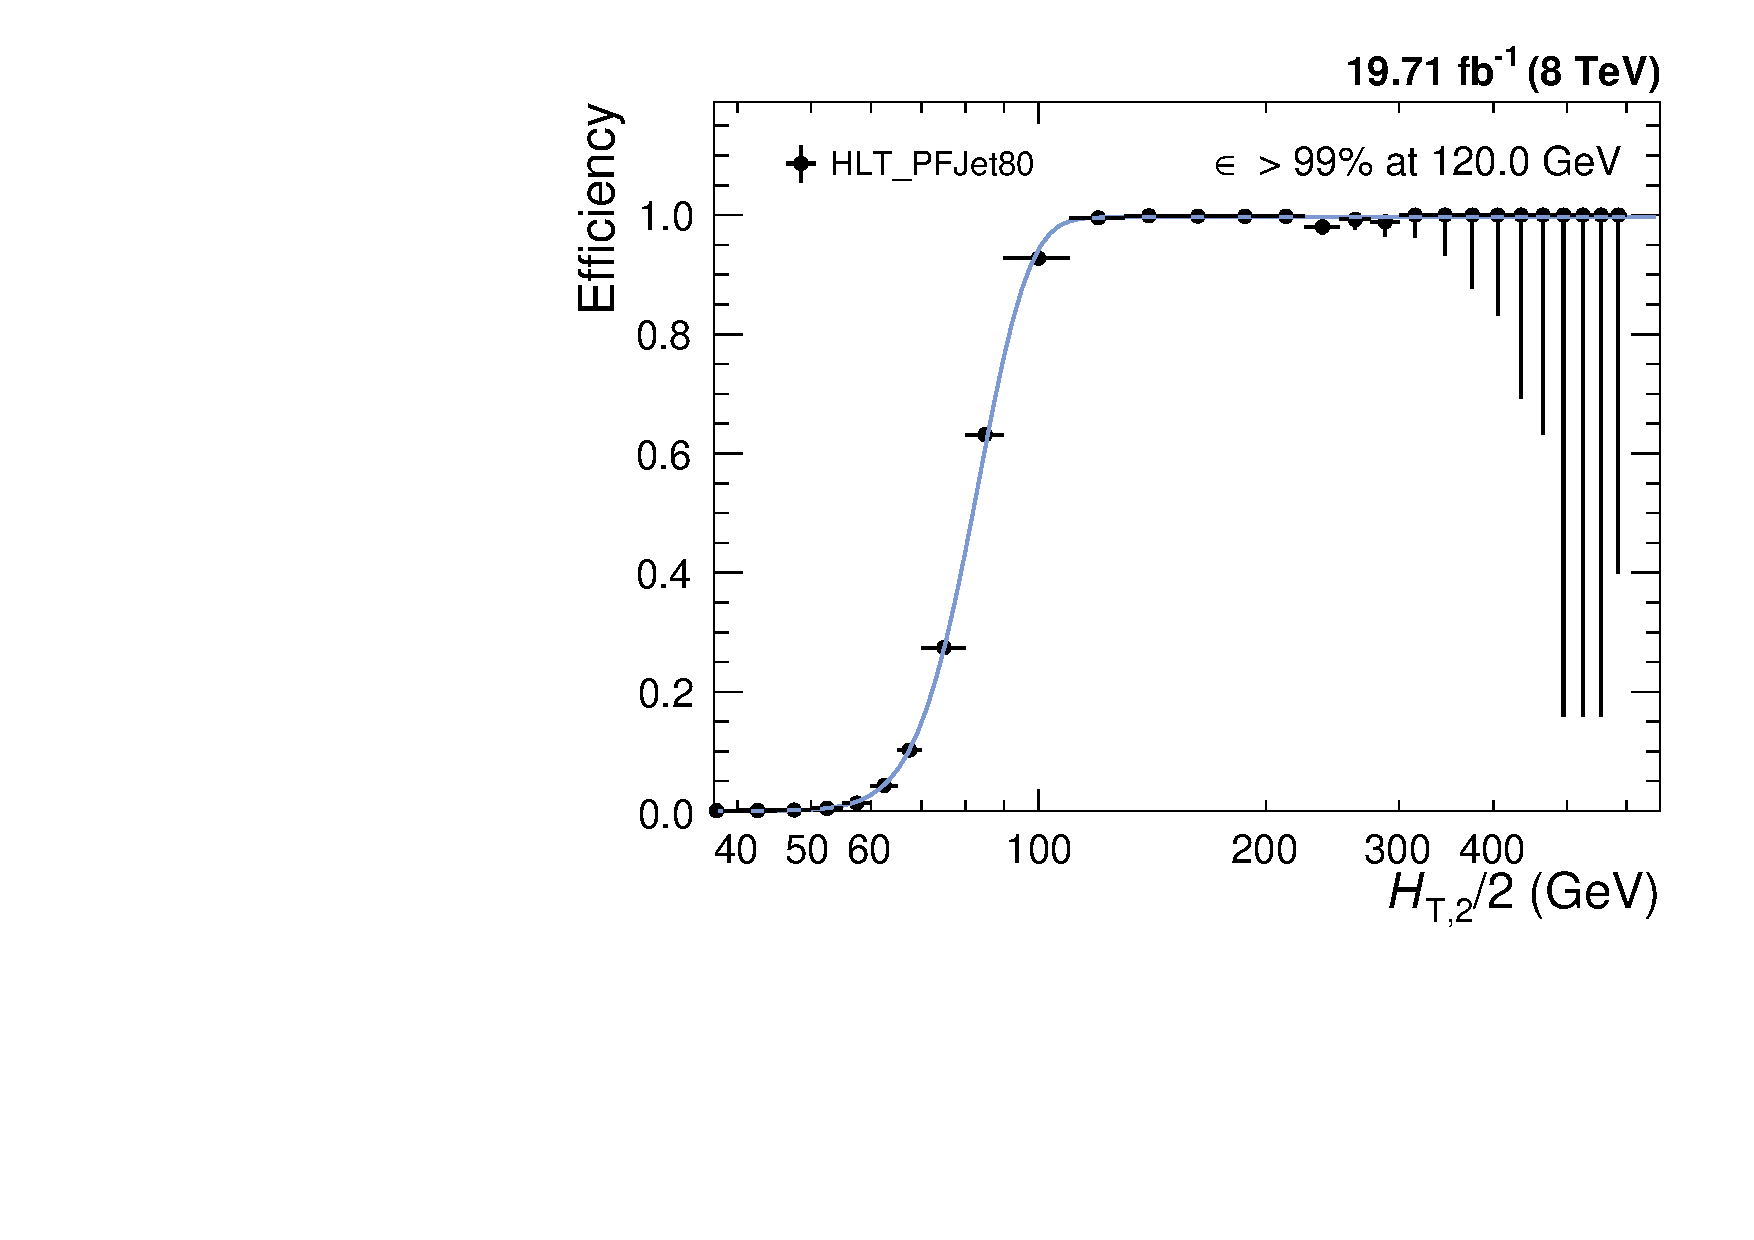
\includegraphics[scale = 0.205]{Plots_HT_2_150/Fit_Turn_Efficiency_80_2_ht_2.pdf}%
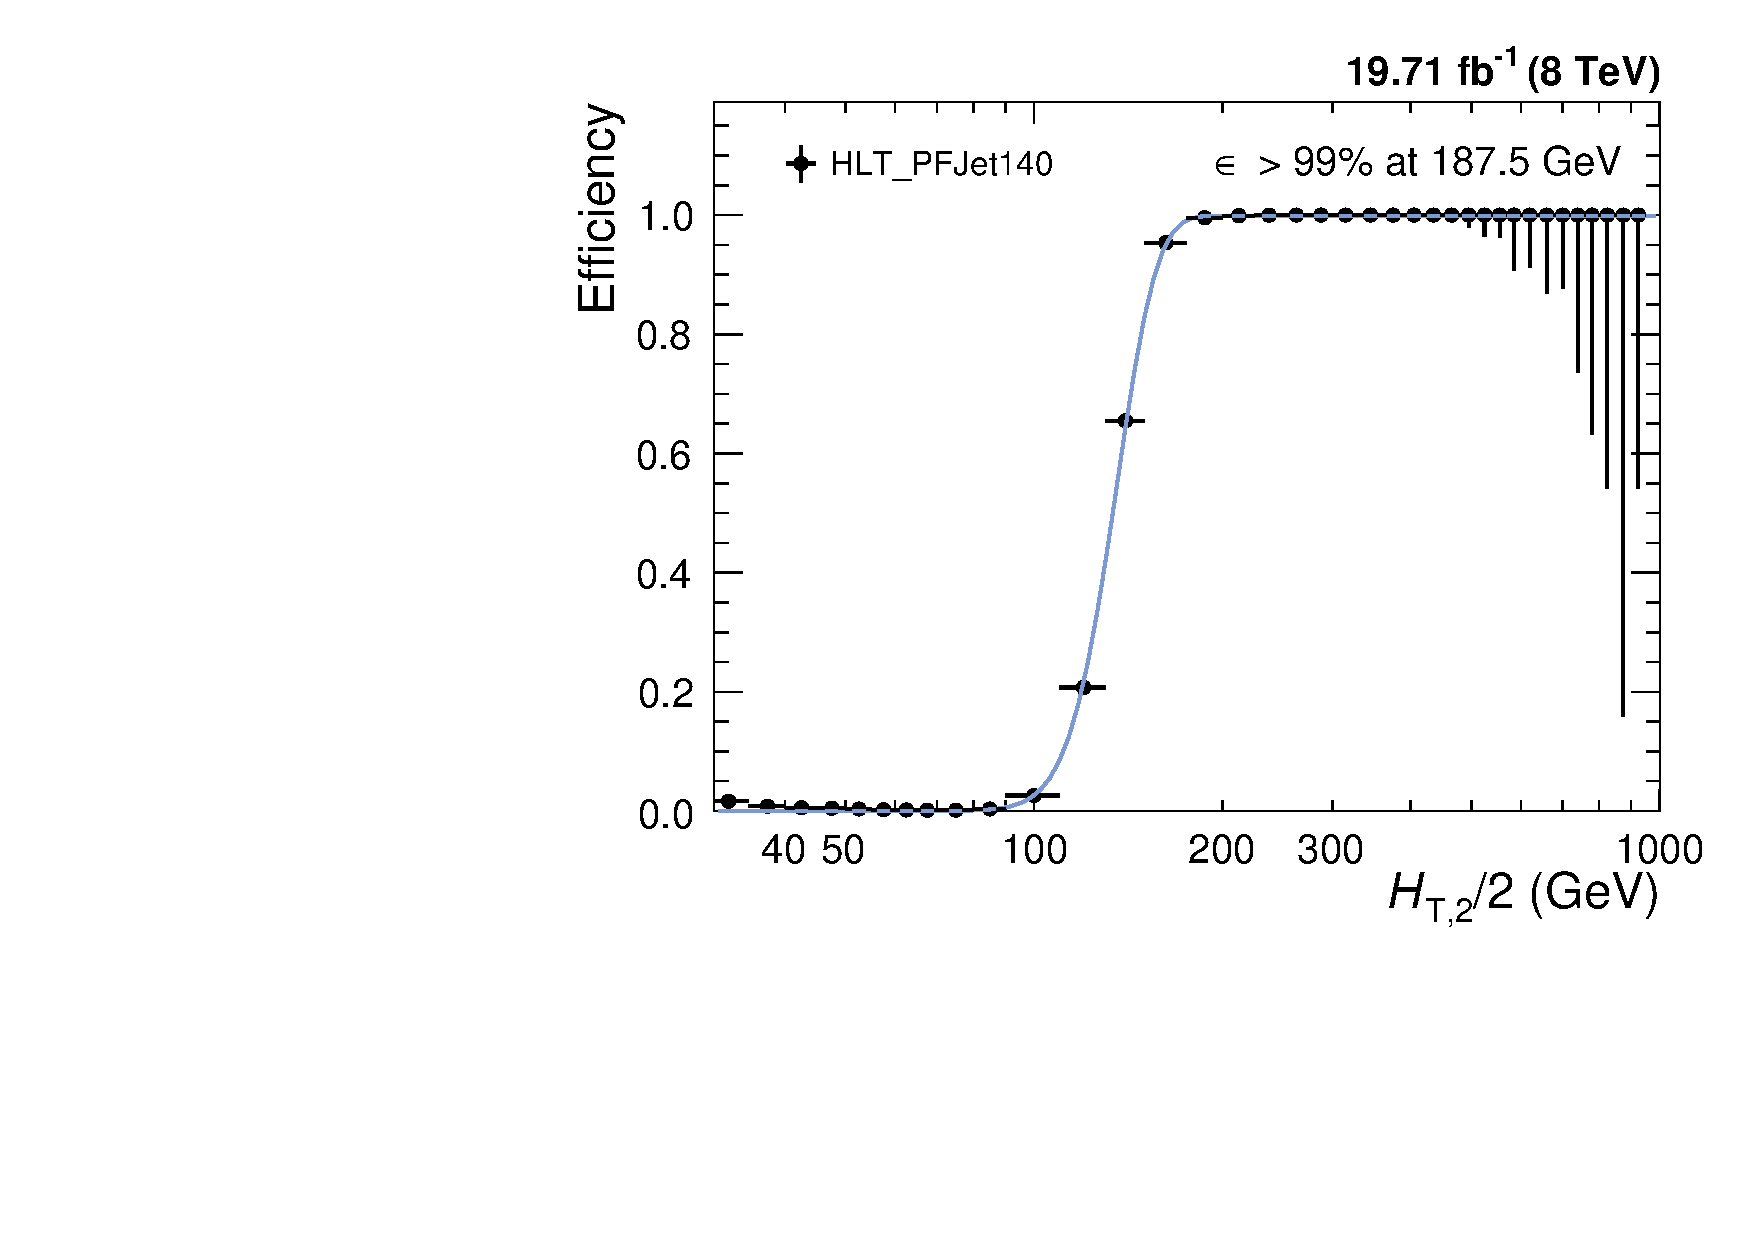
\includegraphics[scale = 0.205]{Plots_HT_2_150/Fit_Turn_Efficiency_140_2_ht_2.pdf}%
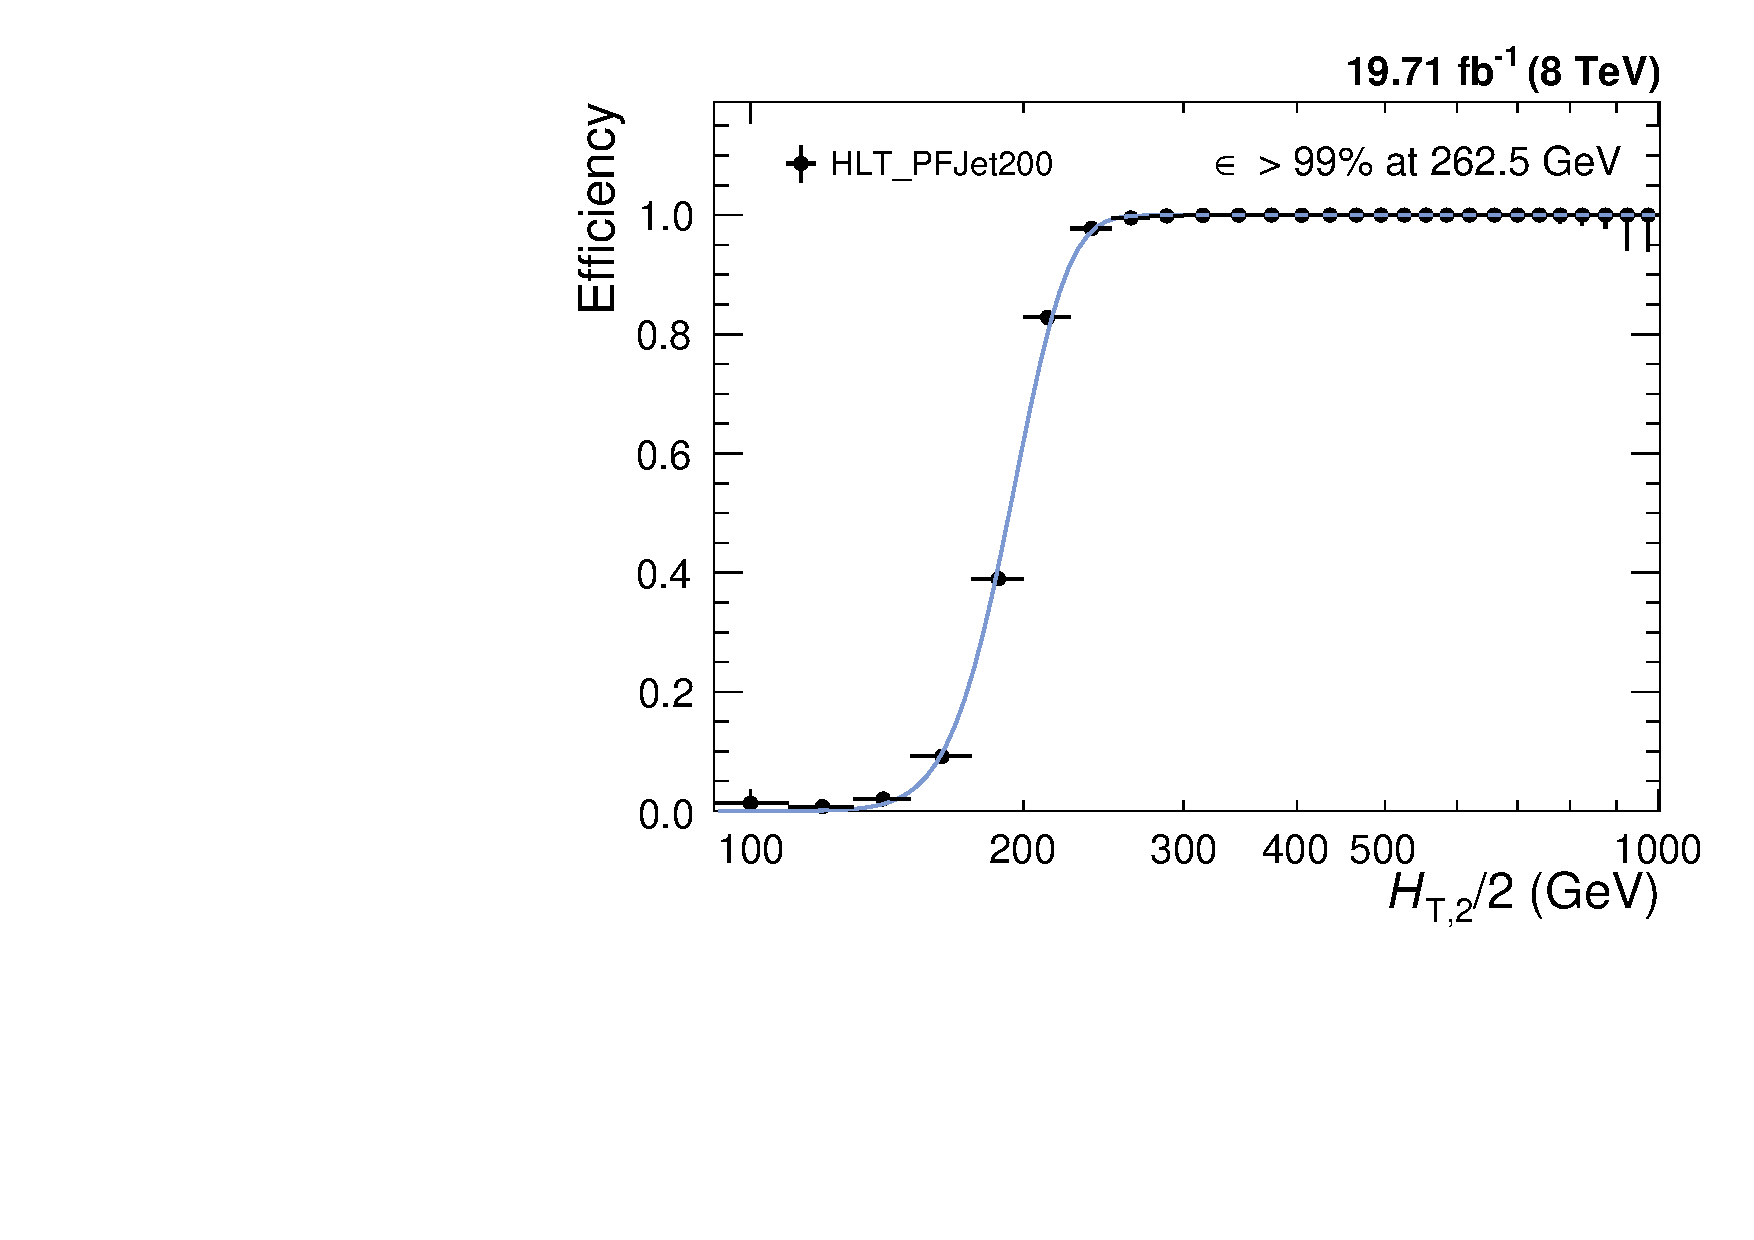
\includegraphics[scale = 0.205]{Plots_HT_2_150/Fit_Turn_Efficiency_200_2_ht_2.pdf}\\
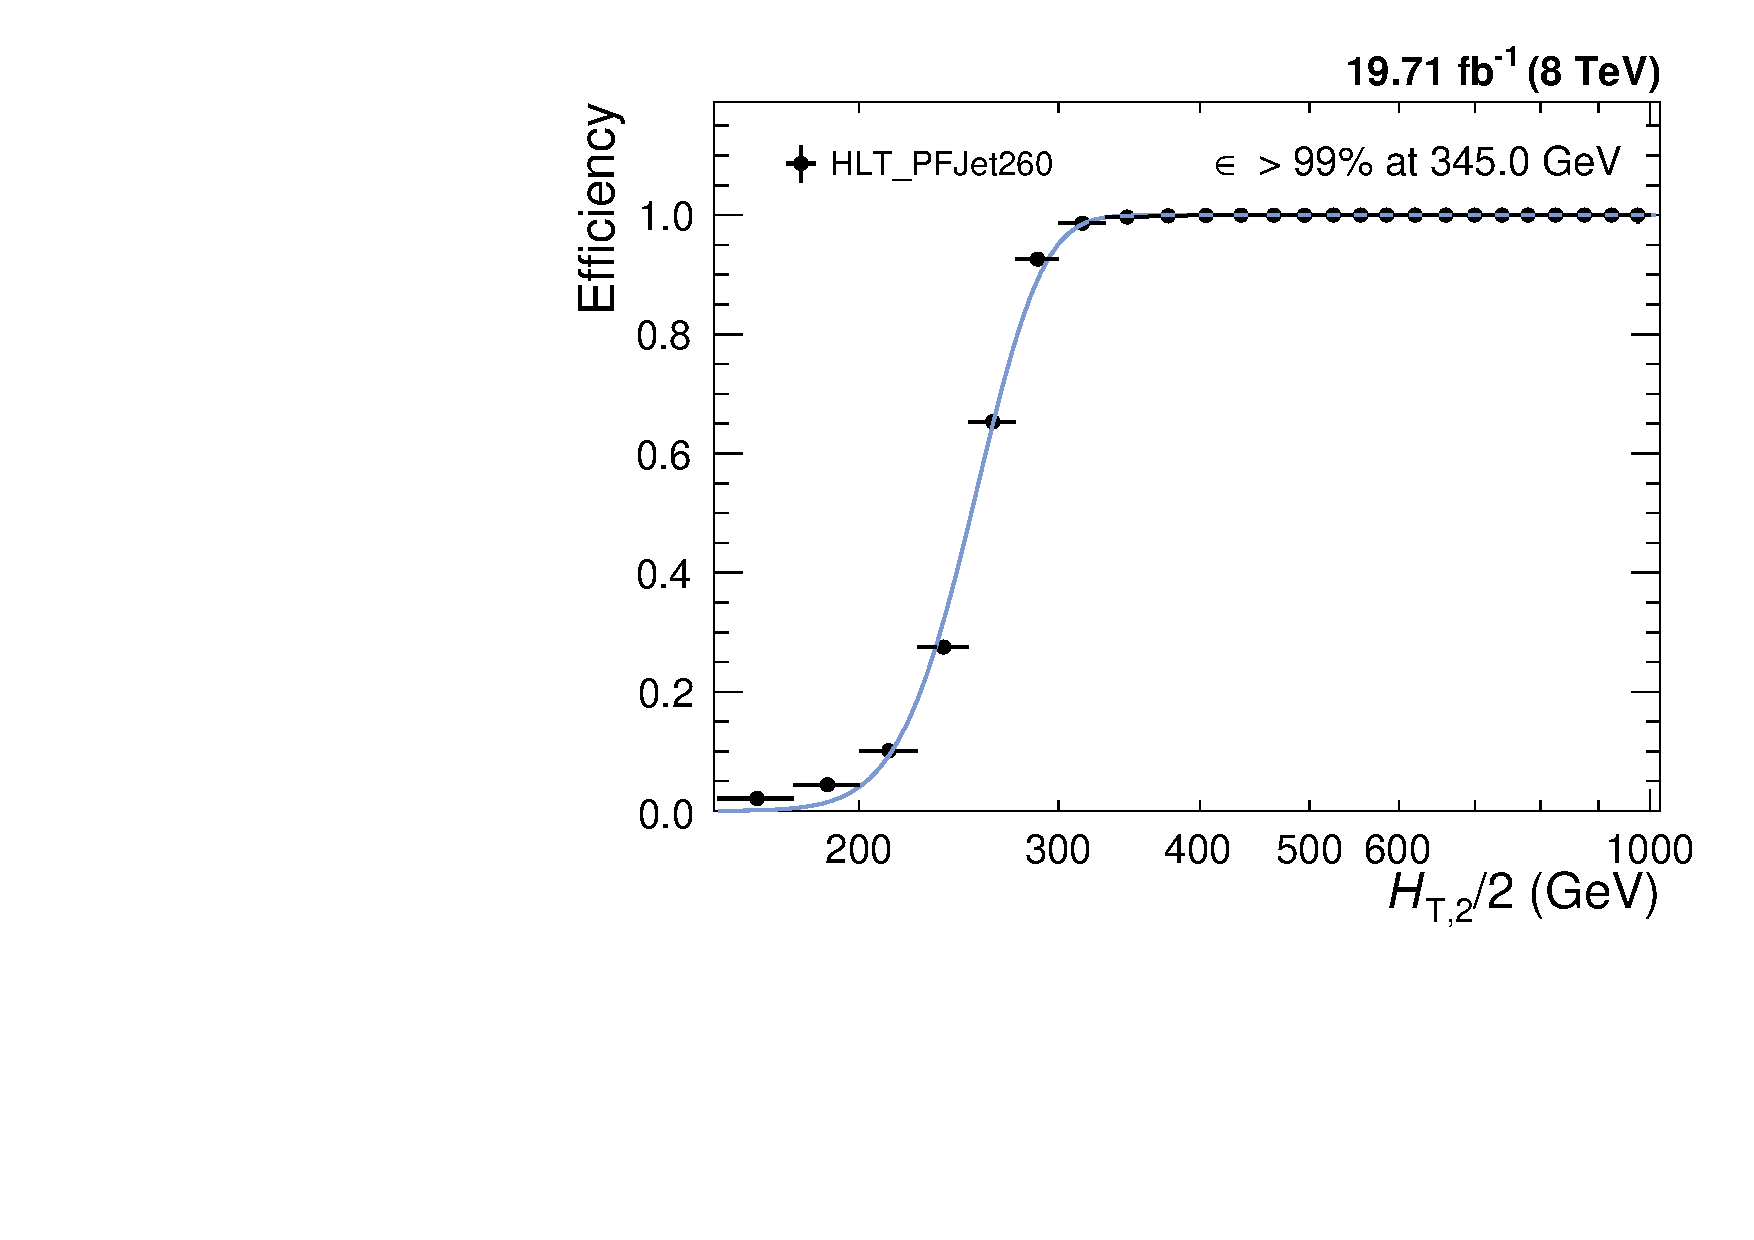
\includegraphics[scale = 0.205]{Plots_HT_2_150/Fit_Turn_Efficiency_260_2_ht_2.pdf}%
\begin{overpic}[scale = 0.205]{Plots_HT_2_150/Fit_Turn_Efficiency_320_2_ht_2.pdf}
\put(-120,-12){\scriptsize {\bf Uncertainty on the efficiency is
calculated using Clopper-Pearson confidence intervals :}}
\put(-30,-23){\scriptsize \blue{$ f_{fit} (x) = \frac {1}{2} \Big( 1 ~\plusn~ {\rm erf} \big(\frac {x - \mu}{\sqrt{2} \sigma} \big) \Big) $}}
\end{overpic}
\end{center}
\end{frame}

%##################################### Slide :  ###########################################
\begin{frame}
\frametitle{\centerline{Missing Transverse Energy}}
\setlength\labelsep {\dimexpr\labelsep + 0.05em\relax}
\setlength\leftmargini{\dimexpr\leftmargini + 0.05em\relax}
\vspace{-8mm}
\begin{center}
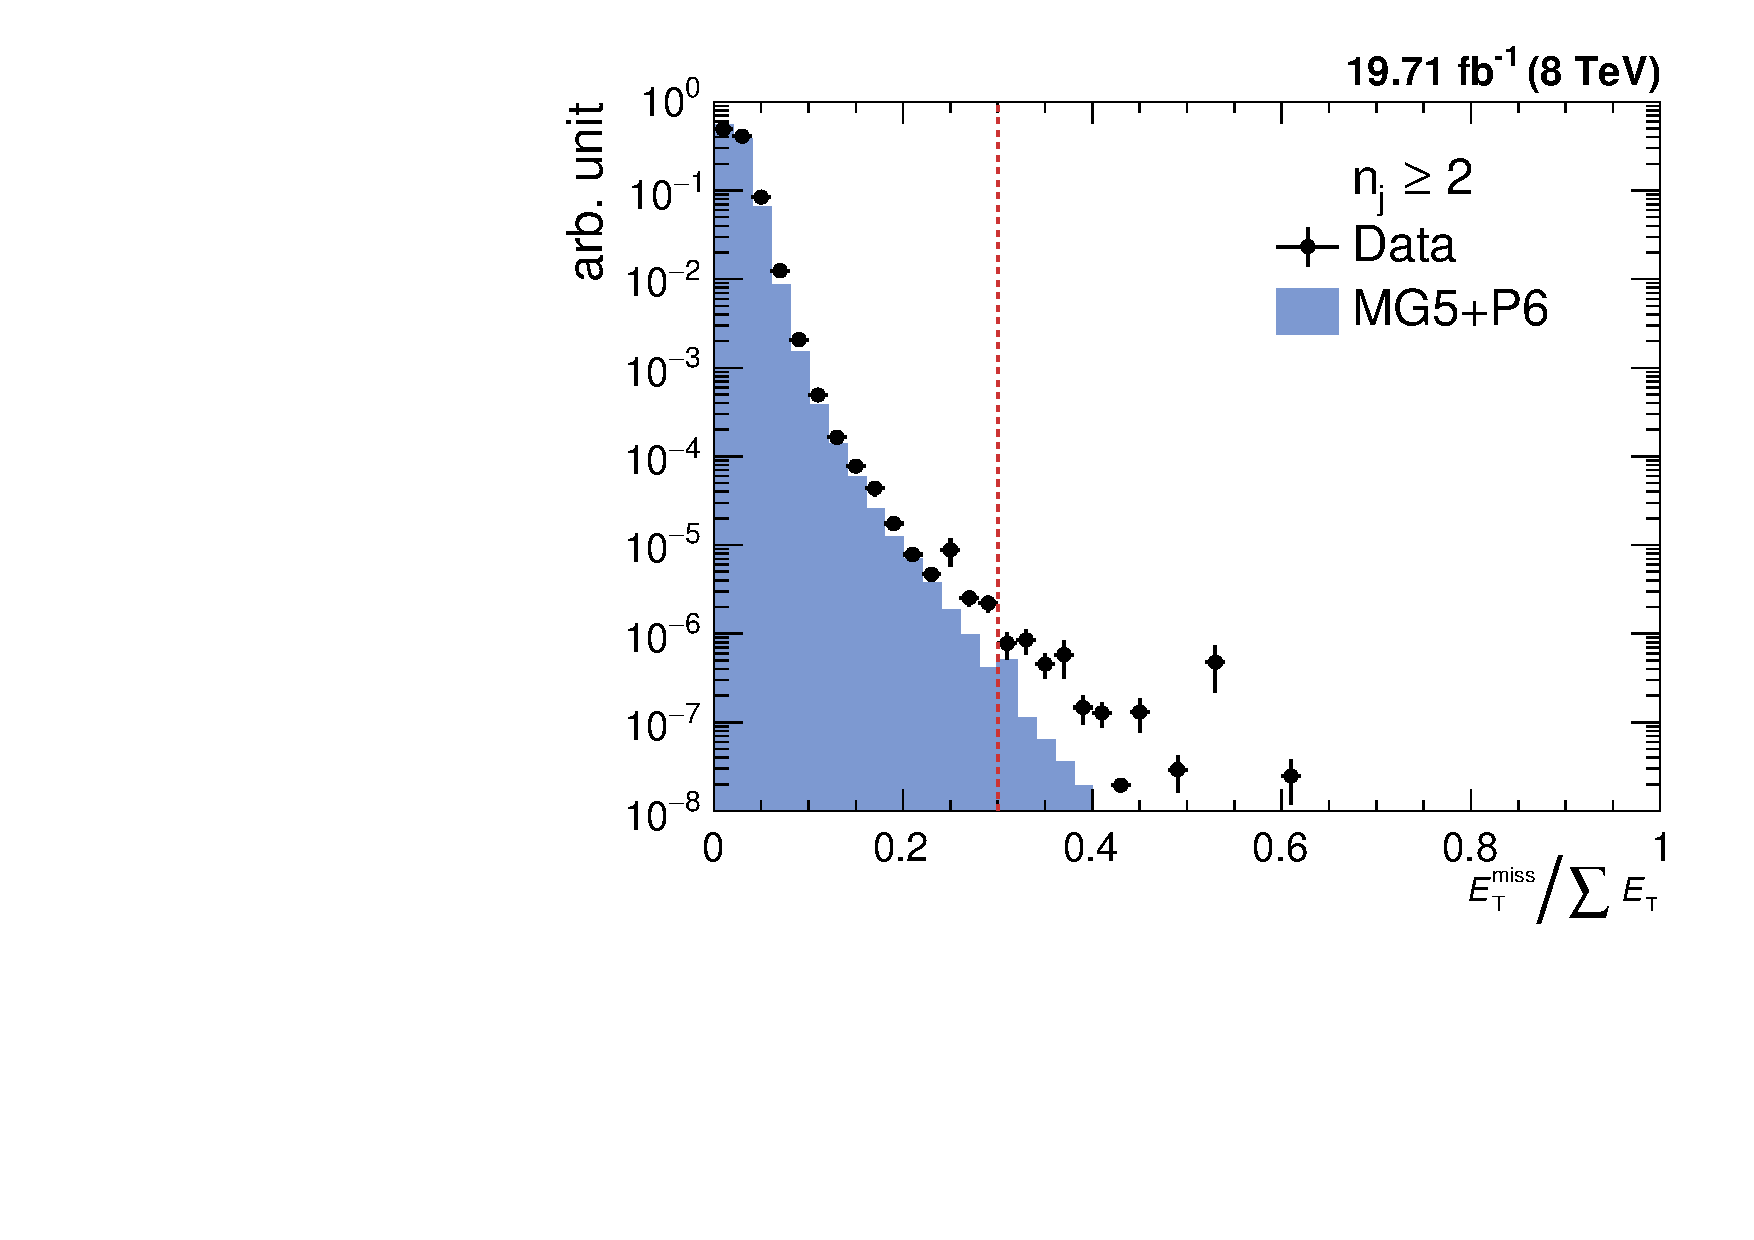
\includegraphics[width=0.51\textwidth]{Plots_HT_2_150/Missing_ET_2.pdf}%
 ~~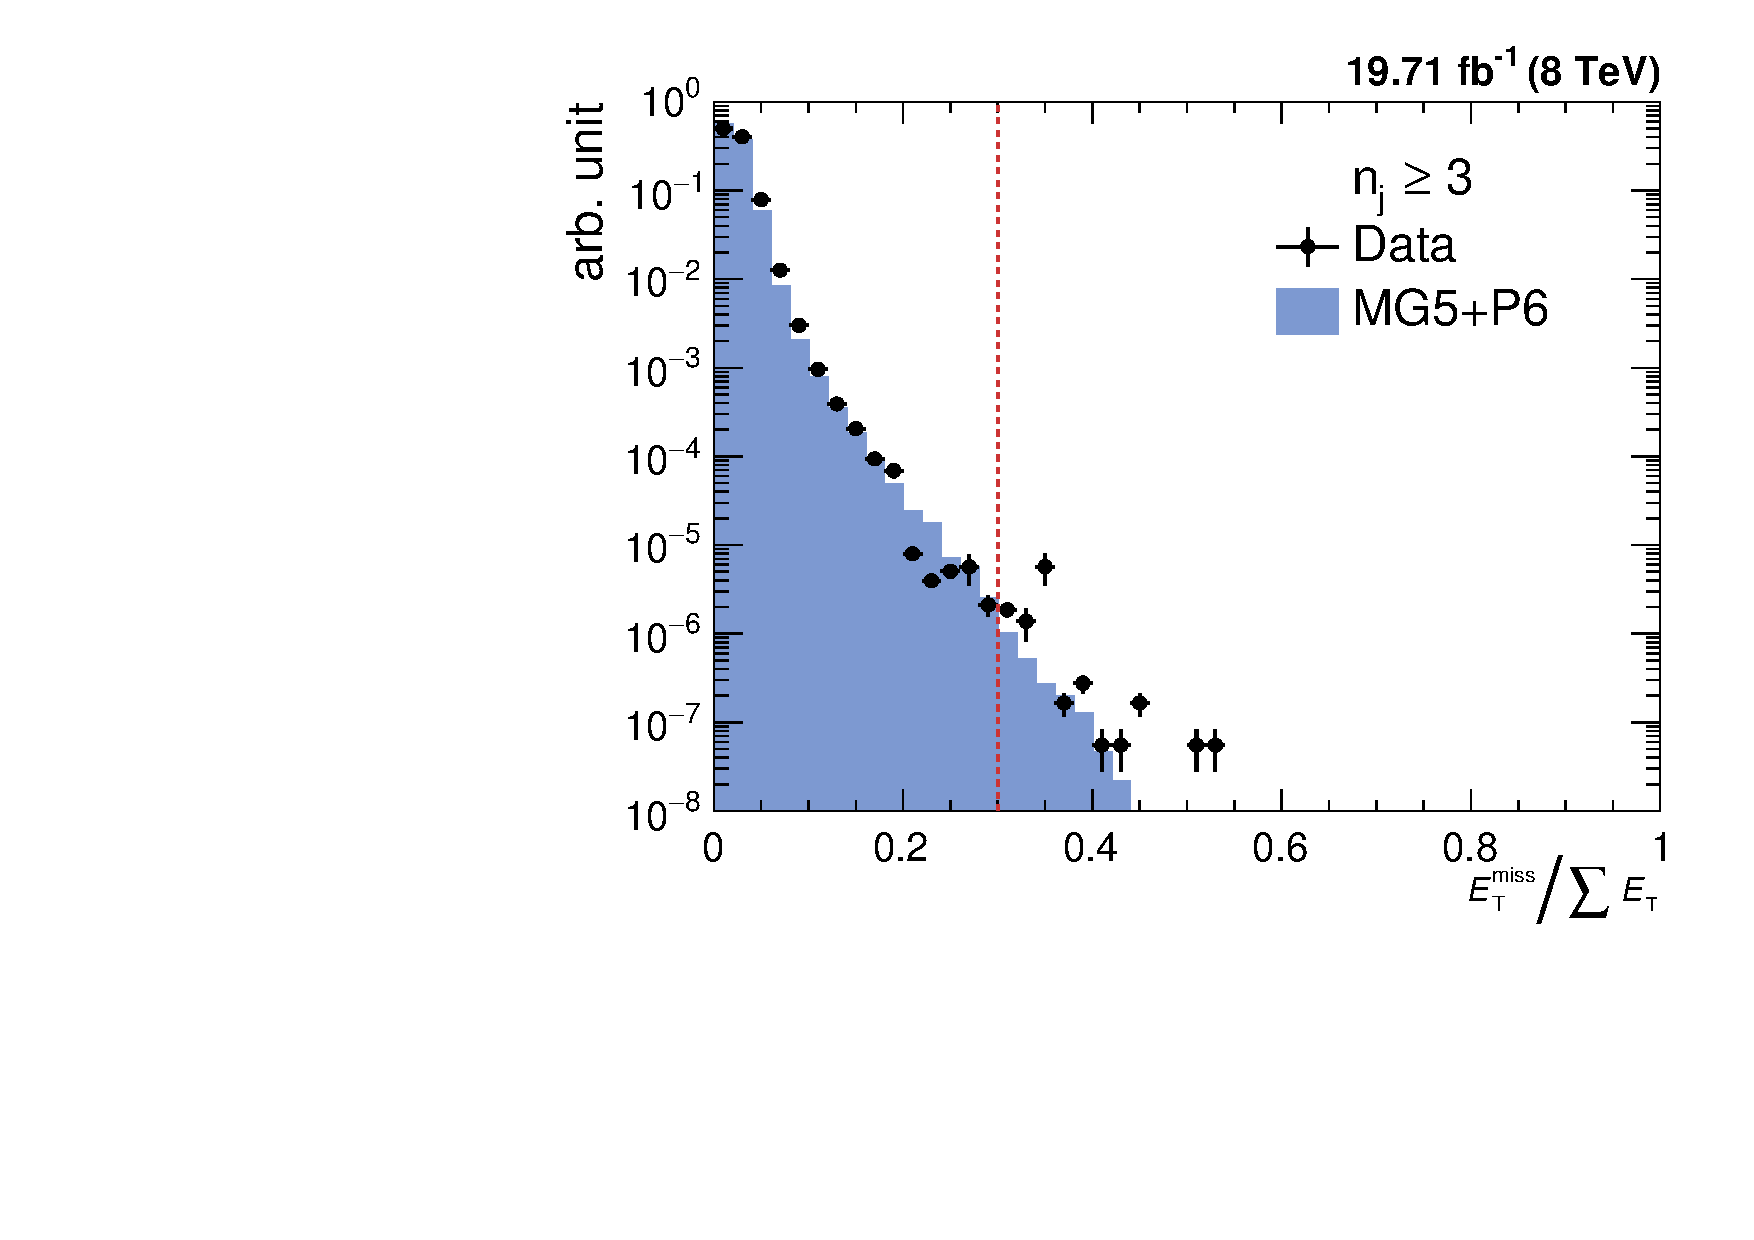
\includegraphics[width=0.51\textwidth]{Plots_HT_2_150/Missing_ET_3.pdf}
\end{center}
\end{frame}

%##################################### Slide : 21 ###########################################
\begin{frame}
\frametitle{\centerline{Simulation and Reconstruction}}
\setlength\labelsep {\dimexpr\labelsep + 0.05em\relax}
\setlength\leftmargini{\dimexpr\leftmargini + 0.05em\relax}
\vspace{-1mm}
\begin{itemize}
\item {\scriptsize \mycolor{Detector Simulation -} a computer program which takes the particles generated by MC event generators. \\}
\tri
\begin{itemize}
\item {\scriptsize Defines the detector system, its geometry, material and electronics properties.
\vspace{0.5mm}
%\item It describes the nature of the interactions of the particles with the material of the detector.
\item \blue{Full Simulation -} based on a C\plusn\plus simulation toolkit \GEANTfour~(GEometry ANd Tracking); handles the interactions of particles with matter over a wide range of energy.
\vspace{0.5mm}
\item \blue{Fast Simulation -} detector effects are parametrized instead of simulating; events are produced at much faster rates.\\}
\end{itemize}
\ball
\item {\scriptsize \mycolor{Digitization :} The simulated detector response is then transformed into a digital signal with the help of electronics.
\vspace{0.5mm}
\item \mycolor{Event Reconstruction :} identifies the particles passing through the detector by interpreting the electrical signals produced in digitization.\\}
\tri
\begin{itemize}
\item {\scriptsize Analysis-level objects are created by combining recorded signals from the tracker, energy deposits from calorimeters and muon detectors.
\vspace{0.5mm}
%\item The reconstructed hits are collected which are combined to form tracks and calorimetric towers. 
%\item Higher level objects such as electrons, muons, photons and jets are reconstructed by combining the tracks and energy deposits.
\item \blue{Particle Flow (PF) Algorithm} combines the information from individual sub-detectors. \\}
\end{itemize}
\ball
\item {\scriptsize \mycolor{Track Reconstruction :} CMS uses an iterative tracking algorithm.\\}%, the Combinatorial Track Finder (CTF) algorithm.\\}
\tri
\begin{itemize}
\item {\scriptsize Quality criteria is used to reject the badly reconstructed tracks and to decrease the fake rate.\\}
\end{itemize}
\ball
\item {\scriptsize \mycolor{Primary Vertex Reconstruction :} identification of the primary vertex of the main hard interaction is crucial. \\}
\tri
\begin{itemize}
\item {\scriptsize Track assigned to only one vertex $\rightarrow$ {\bf hard interaction}. 
\vspace{0.5mm}
\item Track assigned to more than one vertex $\rightarrow$ {\bf soft interaction}.\\}
\end{itemize}
\ball
\end{itemize}
\end{frame}

%##################################### Slide : 22 ###########################################
\begin{frame}
\frametitle{\centerline{Jet Reconstruction}}
\setlength\labelsep {\dimexpr\labelsep + 0.05em\relax}
\setlength\leftmargini{\dimexpr\leftmargini + 0.05em\relax}
\begin{itemize}
\item {\scriptsize PF event reconstruction algorithm converts the detector signals back to physical objects and their energy is measured :\\}
\end{itemize}
\begin{minipage}[thbp]{0.52\textwidth} 
\begin{itemize}
\item []
\tri
\begin{itemize}
\item {\scriptsize {\bf Electrons :} from the track momentum, corresponding ECAL energy deposits and the energy sum of all bremsstrahlung photons associated with the tracks. 
\vspace{0.5mm}
\item {\bf Muons :} from the curvature of the tracks in tracker and muon chambers.
\vspace{0.5mm}
\item {\bf Photons :} directly from the ECAL measurements.\\}
\end{itemize}
\end{itemize}
\end{minipage}
\begin{minipage}[thbp]{0.22\textwidth} 
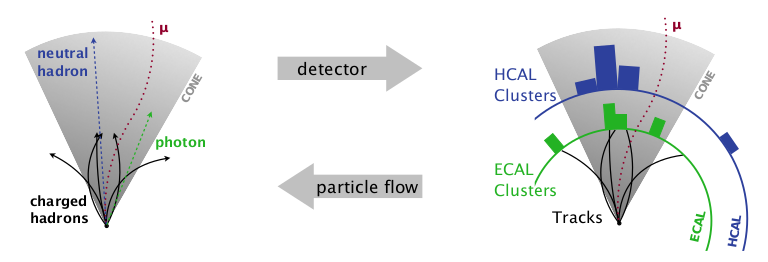
\includegraphics[scale=0.3]{/home/anter/Desktop/Thesis/Figures/Final/PF.png}
\end{minipage}
\begin{itemize}
\item []
\tri
\begin{itemize}
\item {\scriptsize {\bf Charged hadrons} : from track momentum and corresponding energy clusters in ECAL and HCAL. 
\vspace{0.5mm}
\item {\bf Neutral hadrons} : from calibrated ECAL and HCAL energies. \\} 
%\item {\bf Missing transverse energy (\ETmiss) :} \ETmiss = $-\sum\limits_{\rm i}^{}\overrightarrow{p_{\rm T,i}}$. \\}
\end{itemize}
\ball
\item {\scriptsize {\bf Jets :} are reconstructed from the collection of PF objects.\\}
\tri
\begin{itemize}
\item {\scriptsize {\bf Generator Jets (GenJets) :} stable particles generated by the MC event generators.
\vspace{0.5mm}
\item {\bf Calorimetric Jets (CaloJets) :} energy deposits in the ECAL and HCAL towers.
\vspace{0.5mm}
\item \blue{Particle Flow Jets (PFJets) :} detector level jets from particle flow candidates. \\}
\cir
\begin{itemize}
\item {\scriptsize Use of the tracker and high granularity of the ECAL gives better energy resolution.
\item PFJets perform better than CaloJets and are the standard jets used at CMS.\\}
\end{itemize}
\end{itemize}
\end{itemize}
\ball
\end{frame}
%##################################### Slide : 27 ###########################################
\begin{frame}
\label{corr}
\frametitle{\centerline{Jet Energy Corrections}}
\setlength\labelsep {\dimexpr\labelsep + 0.05em\relax}
\setlength\leftmargini{\dimexpr\leftmargini + 0.05em\relax}
\begin{itemize}
\item {\scriptsize \mycolor{Pileup Corrections}\\}
\begin{itemize}
\tri
\item {\scriptsize Due to additional p-p collisions within the same bunch-crossing.
%\item The particles produced from the pileup events get clustered into the jets coming from the hard interaction and increase the jet energy.
\item Corrections are determined by simulating a sample of QCD dijet events with and without pileup effects. 
\item $c_{\rm pileup}$ is calculated from jet area method using the pileup density $\rho$ in the event and the jet area ${\rm A}_{j}$.\\}
\end{itemize}
\ball 
\item {\scriptsize \mycolor{MC Corrections}\\}
\begin{itemize}
\tri
\item {\scriptsize Due to the inefficiencies introduced by the detector simulation.
\vspace{0.5mm}
\item Based on MC simulated QCD events.
\vspace{0.5mm}
\item $c_{\rm mc}$ is derived by comparing the measured jet \pt~to the particle level jet \pt.\\}
\end{itemize}
\ball
\item {\scriptsize \mycolor{Residual Data Corrections} \\}
\begin{itemize}
\tri
\item {\scriptsize Due to remaining small differences between the data and MC simulations.
\vspace{0.5mm} 
\item Applied only to the data.
\vspace{0.5mm}
\item $c_{\rm res}$ is derived from data-driven methods using dijet events in which a probe jet is calibrated using a tag jet.\\}
\end{itemize}
\ball
\item {\scriptsize \mycolor{Flavor Corrections}\\} 
\begin{itemize}
\tri
\item {\scriptsize Correct the jets for flavor dependence (b, $\tau$ etc.) and are optional.
\vspace{0.5mm} 
\item Extracted using Z\plusn jet and photon\plusn jets simulated events.\\}
\end{itemize}
\ball
\end{itemize}
\end{frame}

%##################################### Slide :  ###########################################
\begin{frame}
\label{jer2}
\frametitle{\centerline{Jet Energy Resolution (JER)}}
\setlength\labelsep {\dimexpr\labelsep + 0.05em\relax}
\setlength\leftmarginiii{\dimexpr\leftmarginiii + 0.05em\relax}
\vspace{-1mm}
\begin{minipage}[thbp]{0.65\textwidth}
\begin{itemize}
 \item {\scriptsize \mycolor{Jet energy resolution (JER)} : Finite value of the resolution of the detector because of differences of the measured quantity from its true value. %Difference of the measured quantity from its true value due to detector noise, uncertainties in the calibration, non-linearity of the response etc.
\vspace{0.5mm}
\item Resolution is given by the width of a Gaussian distribution, centered around the true value of the measured quantity.
\vspace{0.5mm}
\item Due to finite resolution of the CMS detector, the measured \pt~of jets get smeared.
\vspace{0.5mm}
\item Measurements show that JER in data is worse than in the simulation and the reconstructed jet \pt~in MC needs to be smeared more to describe the data.
\vspace{0.5mm}
\item Reconstructed jet \pt~is smeared randomly using a Gaussian function, $f$(\pt) with a width widened by the scaling factor (c$_{central}$) :
\vspace{-5.5mm}
\begin{align*}
\resizebox{.6\hsize}{!}{$ \mycolor{f(p_{\rm T}) = a \times \exp\Bigg(-\frac{1}{2}\Big(\frac{p_{\rm T} - \mu}{\sigma}\Big)^2\Bigg)}$}
\end{align*}\\
\vspace{-1.5mm}
where $a$ is a constant, mean $\mu$ = 0, \\width $\sigma = \sqrt{c^2_{central} - 1} \cdot {\rm JER}$(\pt) $\times$ \pt
\item Width of the response, \mycolor{$R = \frac{{\rm Reco}~\httwot}{{\rm Gen}~\httwot}$}, gives JER.\\}
%\item \blue{Double-sided Crystal Ball function} takes into account the non-Gaussian tails of the jet response distribution. \\}
\end{itemize}
\end{minipage}
\begin{minipage}[thbp]{0.33\textwidth}
\begin{center}
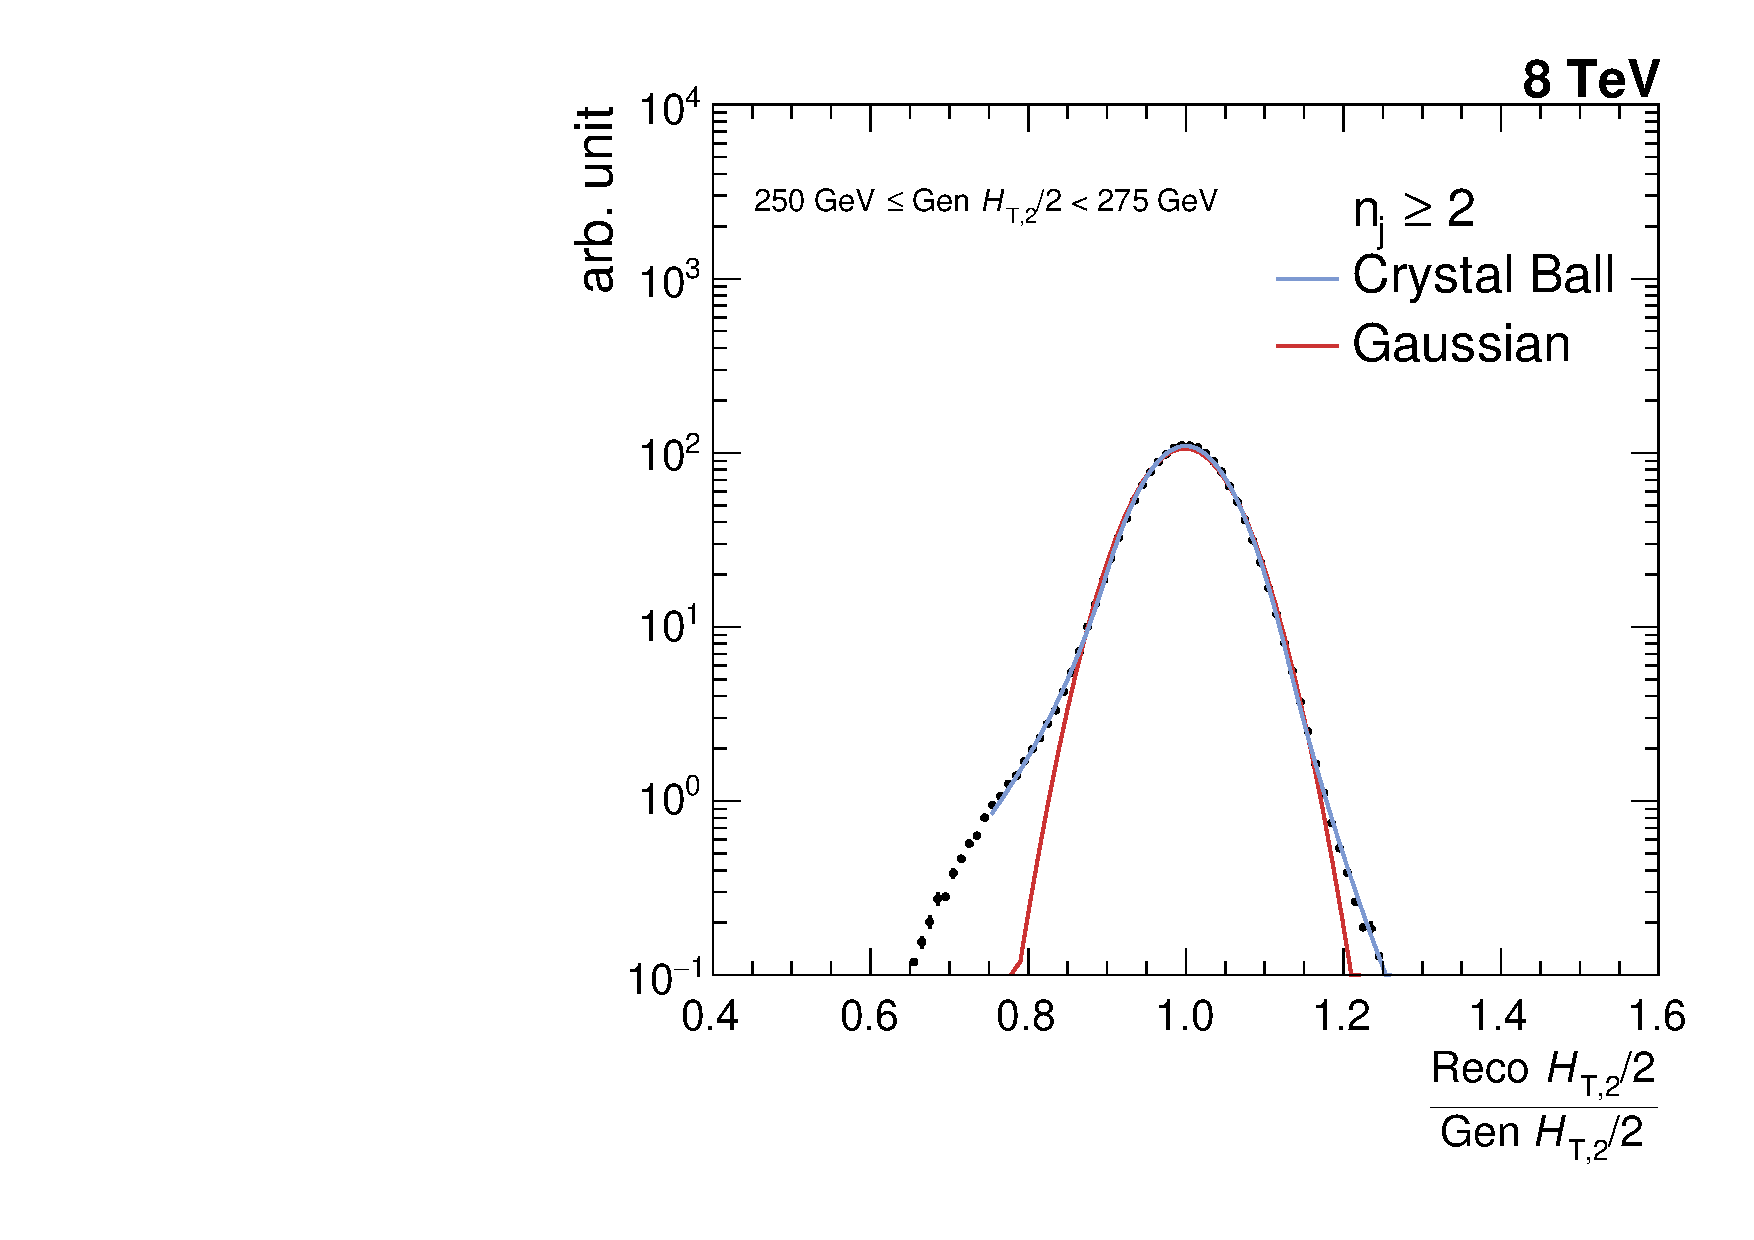
\includegraphics[scale = 0.2]{Plots_HT_2_150/Fit_Res_2_final_crystal_genbin_250-275_crystal_nomet.pdf}\\
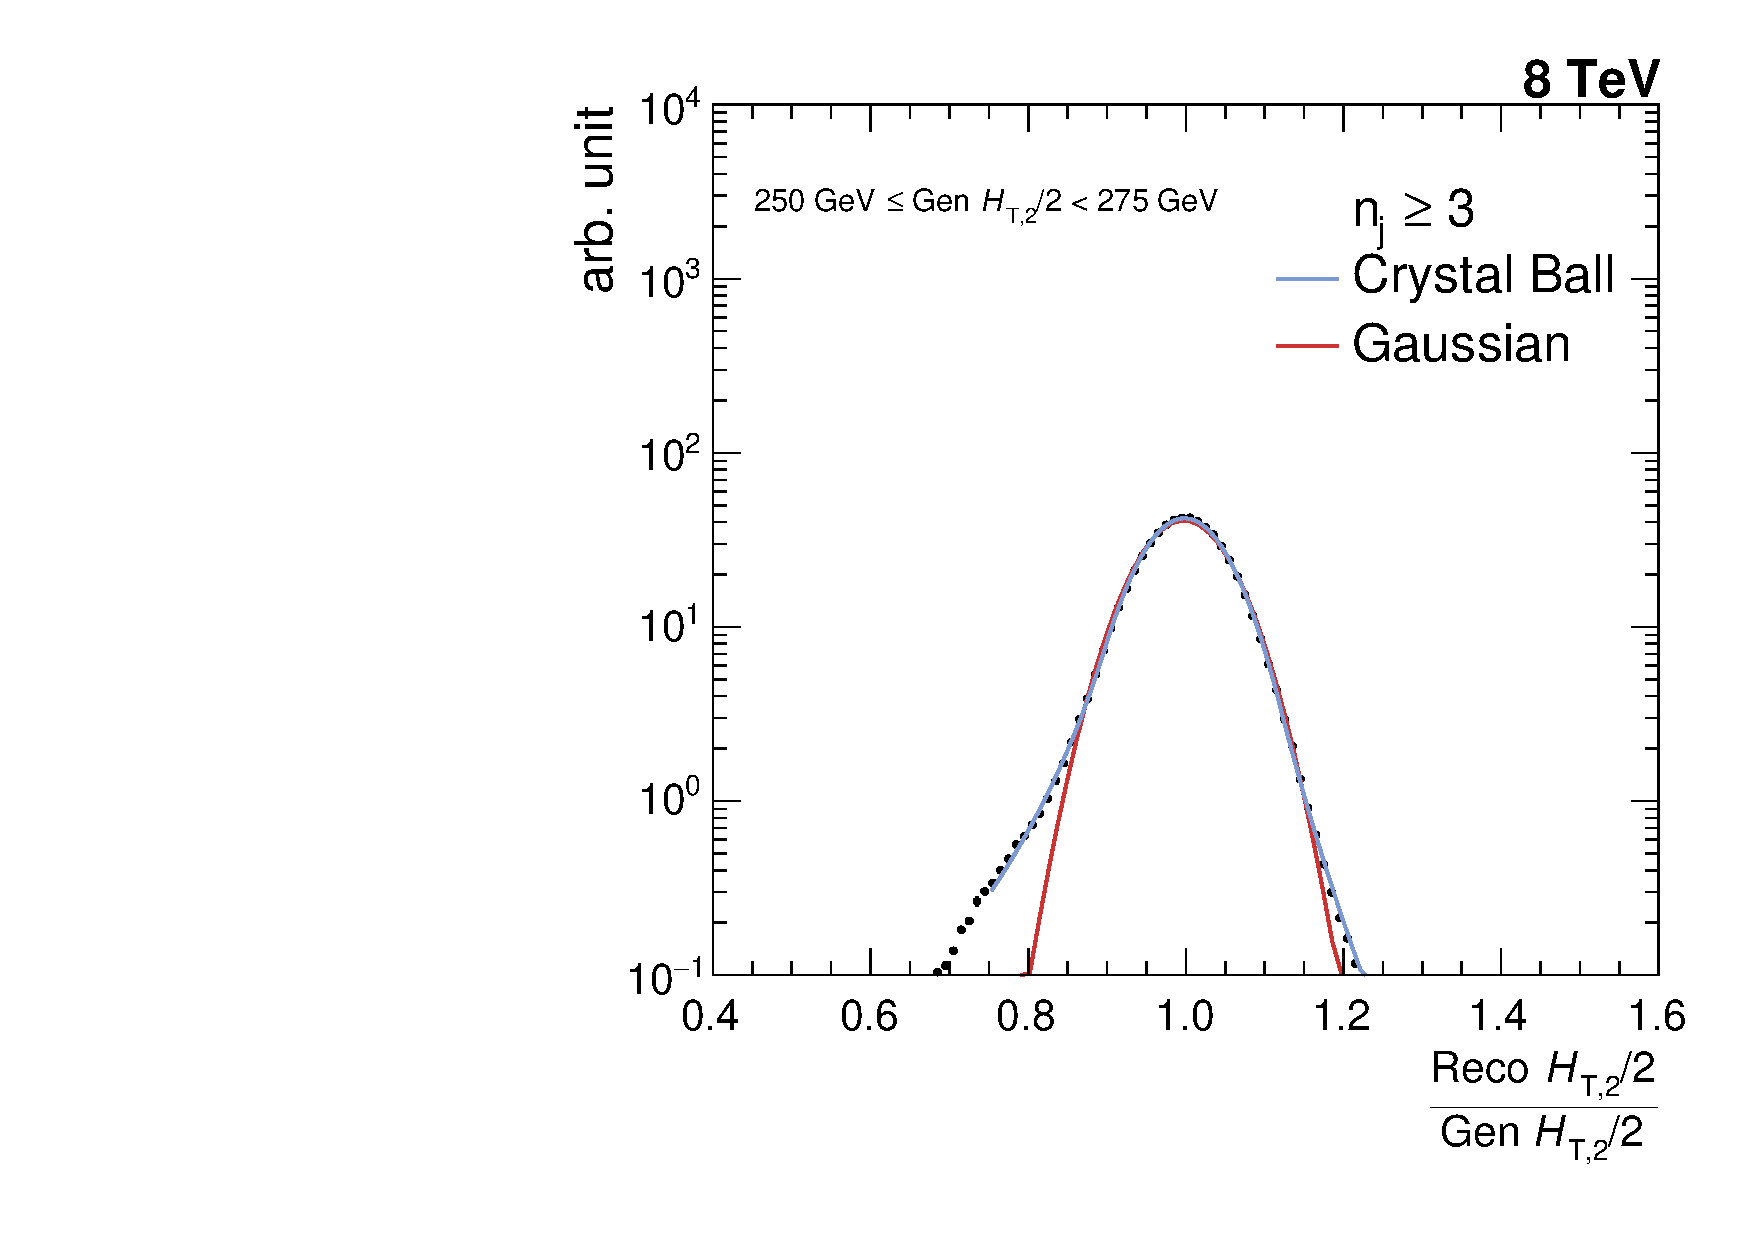
\includegraphics[scale = 0.2]{Plots_HT_2_150/Fit_Res_3_final_crystal_genbin_250-275_crystal_nomet.pdf}\\
\end{center}
\end{minipage}
\vspace{-1mm}
\begin{itemize}
\item {\scriptsize \blue{Double-sided Crystal Ball function} describes the jet response distribution. \\}
\end{itemize}
\end{frame}

%##################################### Slide :  ###########################################
\begin{frame}
\frametitle{\centerline{Crystal Ball Function}}
\setlength\labelsep {\dimexpr\labelsep + 0.05em\relax}
\setlength\leftmargini{\dimexpr\leftmargini + 0.05em\relax}
\vspace{-8mm}
\begin{center}
\begin{itemize}
\item {\scriptsize The Crystal Ball function, developed within the Crystal Ball Collaboration, is a probability density function which is often used as a fitting function in high energy physics. 
\vspace{2mm}
\item This function, described by Eq.~\ref{eq:crystal_ball}, consists of a Gaussian core with separate power-law low-end tails, below a certain threshold. 

\begin{equation}
\label{eq:crystal_ball}
 f = N \cdot \begin{cases}
     e^{-\frac{1}{2}\alpha^2_{L}} \cdot \bigg[\bigg(\frac{\alpha_{L}}{n_L}\bigg)\bigg(\frac{n_L}{\alpha_{L}}-[\alpha_L \plus x]\bigg)\bigg]^{-n_{L}}, & ~~~~~~~~~x < -\alpha_{L}\\
     e^{-\frac{1}{2}x^2}, & -\alpha_{L} \leq x \leq \alpha_{H}\\
     e^{-\frac{1}{2}\alpha^2_{H}} \cdot \bigg[\bigg(\frac{\alpha_{H}}{n_H}\bigg)\bigg(\frac{n_H}{\alpha_{H}}-[\alpha_H \plus x]\bigg)\bigg]^{-n_{H}}, & ~~~~~~~~~x > \alpha_{H}\\
      \end{cases} 
\end{equation}
where $N$ is a normalisation factor, $\alpha_L$ and $\alpha_H$ delimit the Gaussian core, which is replaced by a power-law behaviour proportional to 1/$n_L$ and 1/$n_H$ to the lower and higher side, respectively. 
\vspace{2mm}
\item The Crystal Ball function itself and its first derivative are continuous.\\}
\end{itemize}
\end{center}
\end{frame}

%##################################### Slide :  ###########################################
\begin{frame}
\label{jer1}
\frametitle{\centerline{Jet Energy Resolution (JER)}}
\setlength\labelsep {\dimexpr\labelsep + 0.05em\relax}
\setlength\leftmarginiii{\dimexpr\leftmarginiii + 0.05em\relax}
\vspace{-2mm}
\begin{table}[!htbp]
\centering\tiny
\begin{tabular}{lccccc}
 \hline\hline
$~~~\eta$  & $0.0$ - $0.5$ & $0.5$ - $1.1$ & $1.1$ - $1.7$ & $1.7$ - $2.3$ & $2.3$ - $2.8$  \rbthm\\ \hline

c$_{central}$ & 1.079   & 1.099   & 1.121    & 1.208   & 1.254    \rbtrr\\
c$_{down}$    & 1.053   & 1.071   & 1.092    & 1.162   & 1.192    \rbtrr\\
c$_{up}$      & 1.105   & 1.127   & 1.150    & 1.254   & 1.316    \rbtrr\\ 
 \hline\hline
 \end{tabular}
\end{table}
\begin{itemize}
\item {\scriptsize To match the resolution in the data, the reconstructed jet transverse momentum in simulated events need to be smeared by applying the scale factors. 
\item The uncertainty on the resolution is given by an upwards and downwards variation c$_{up}$ and c$_{down}$ of the measured scaling factor c$_{central}$.\\}
\end{itemize}
\vspace{-6mm}
\begin{center}
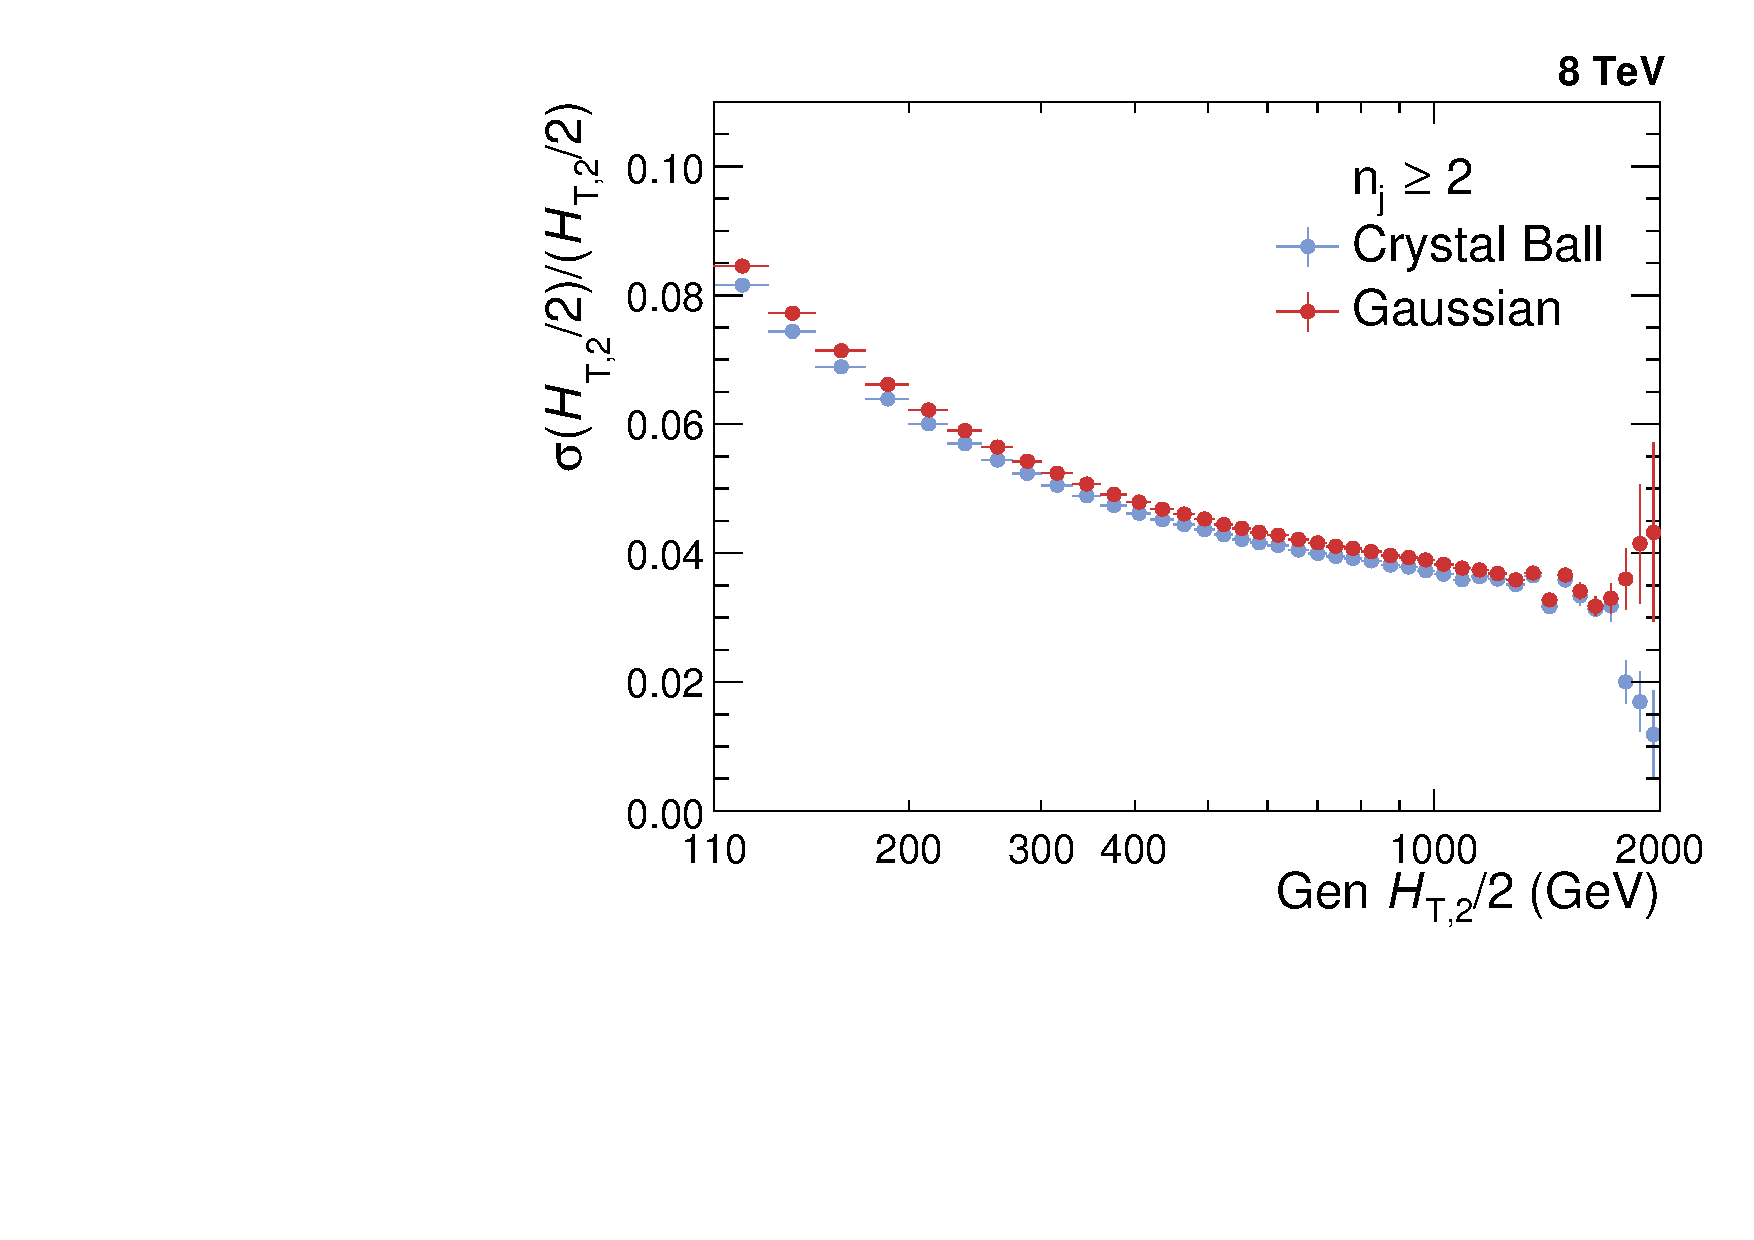
\includegraphics[scale=0.3]{Plots_HT_2_150/Comparison_Resolution_Crystal_Gauss_2.pdf}%
 ~~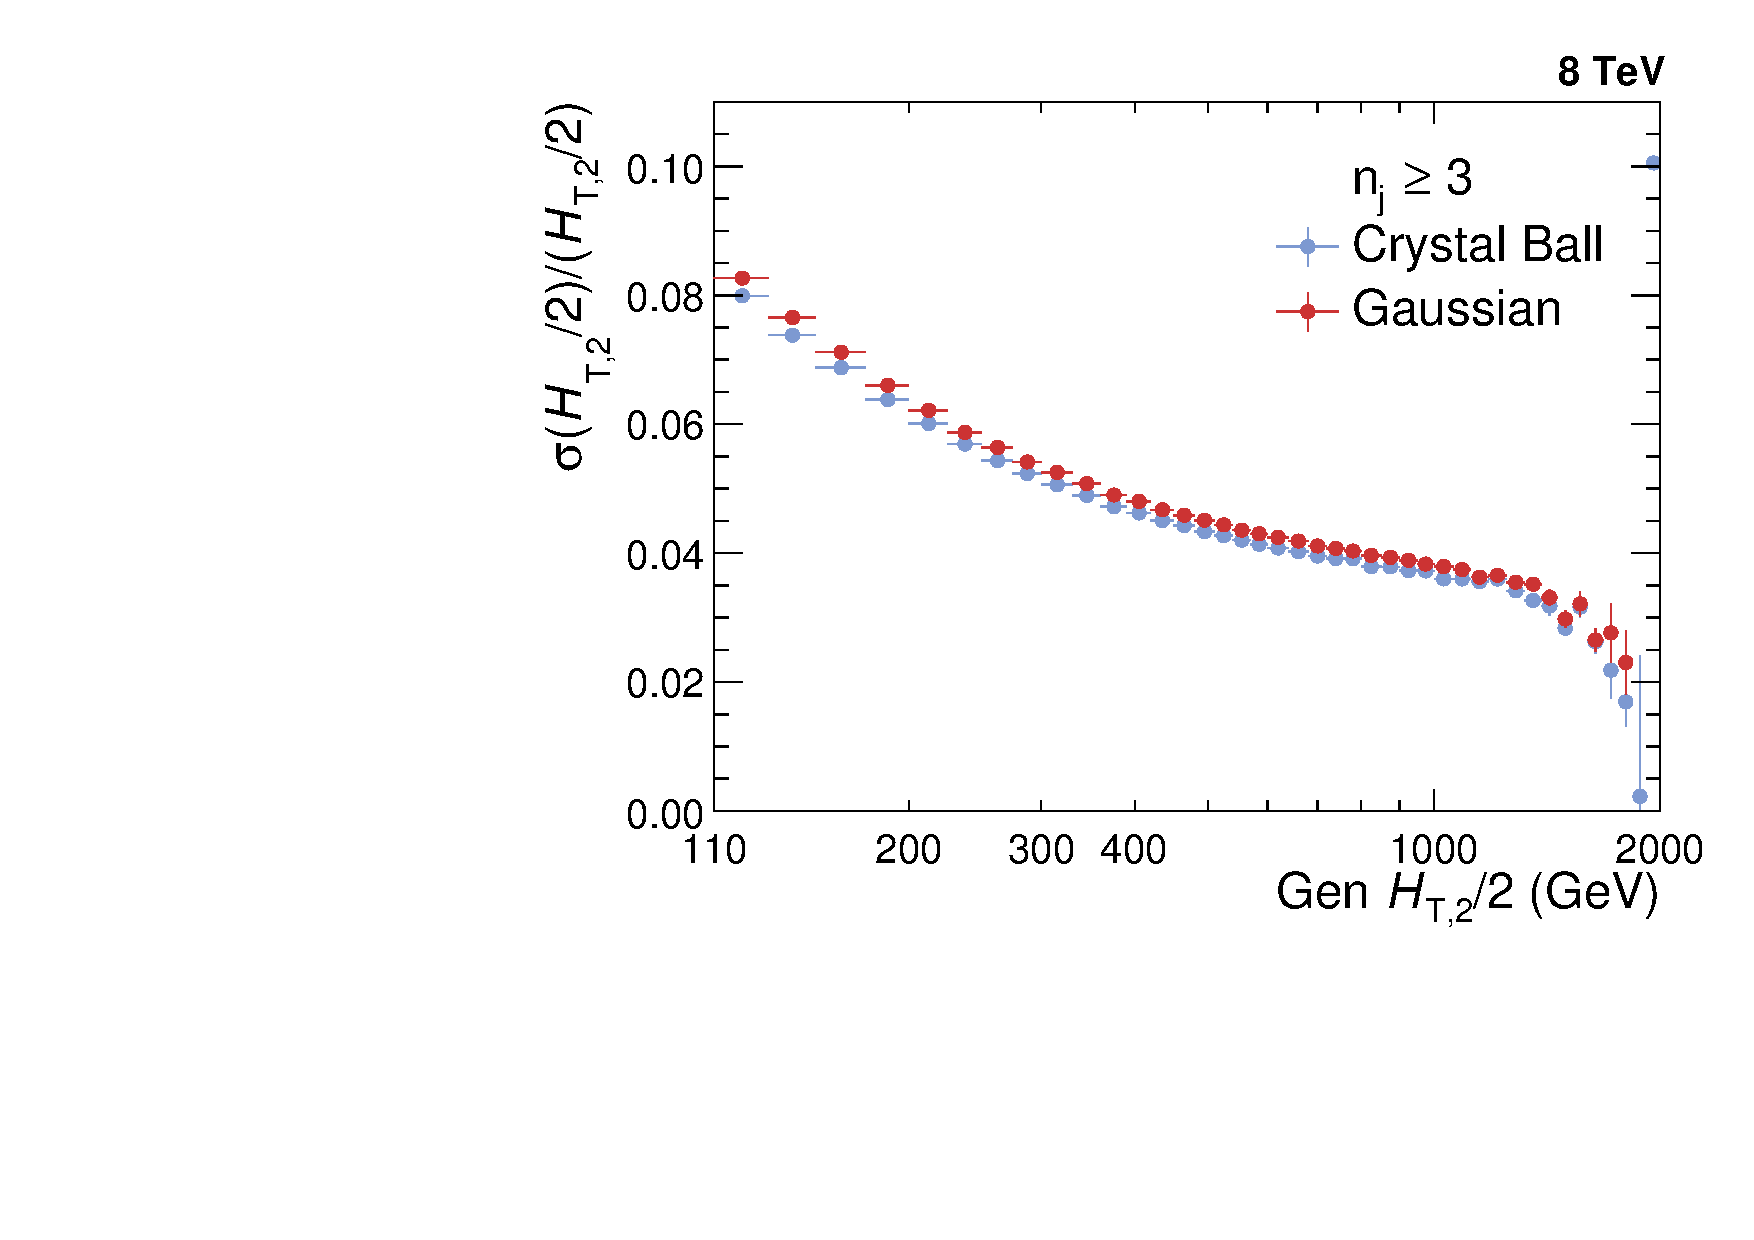
\includegraphics[scale=0.3]{Plots_HT_2_150/Comparison_Resolution_Crystal_Gauss_3.pdf}
\end{center}
\end{frame}

%##################################### Slide :  ###########################################
\begin{frame}
\frametitle{\centerline{Jet Energy Resolution (JER)}}
\setlength\labelsep {\dimexpr\labelsep + 0.05em\relax}
\setlength\leftmarginiii{\dimexpr\leftmarginiii + 0.05em\relax}
\vspace{-2mm}
\begin{center}
\begin{itemize}
 {\scriptsize \item Fit using NSC-formula \mycolor{$\frac{\sigma (x)}{x} = \sqrt{sign(N) \cdot \frac{N^{2}}{x^{2}}+ S^{2} \cdot x^{s-1} + C^{2}}$}; where $x$ = \httwotns. \\
\item Fits at high \httwot start lacking events. \\}
\end{itemize}
\end{center}
\hspace{-3mm}
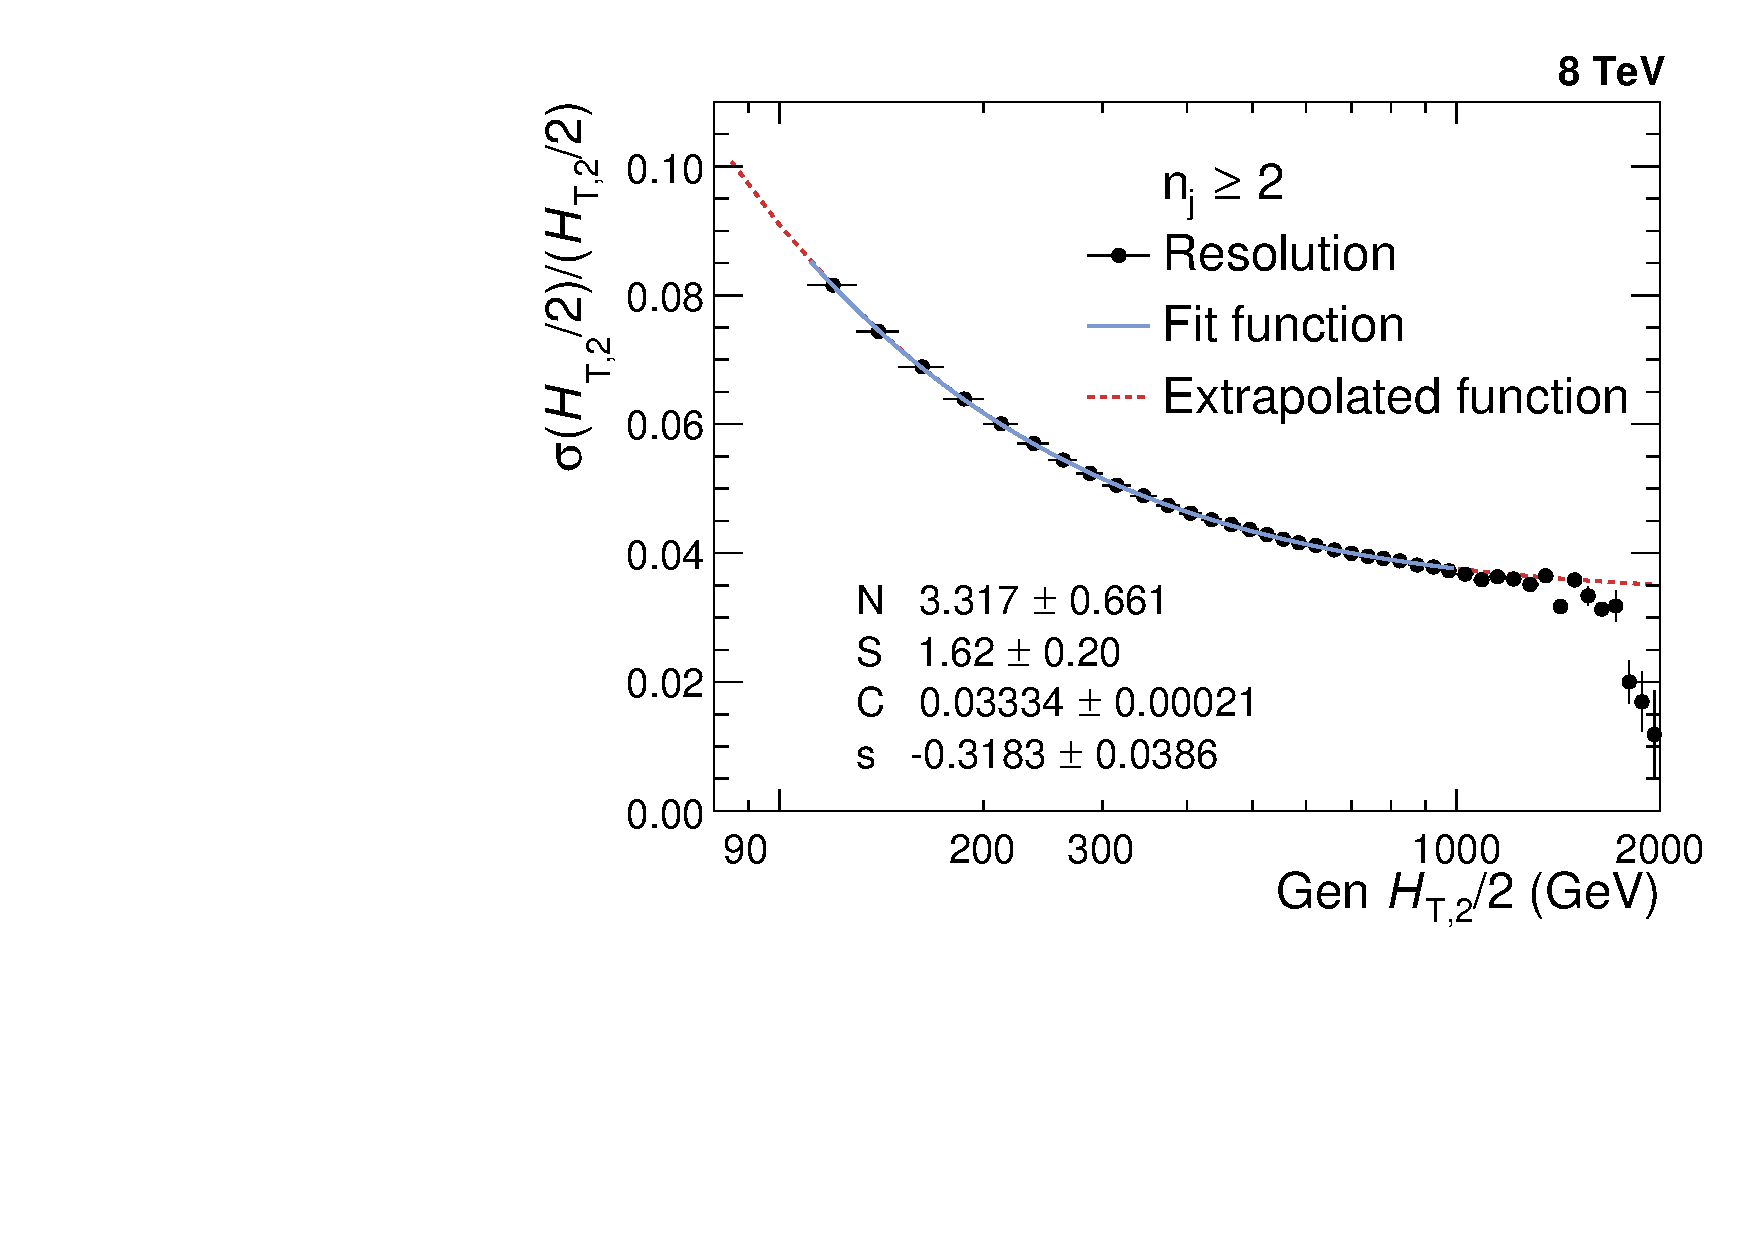
\includegraphics[scale = 0.215]{Plots_HT_2_150/Extrapolate_Sigma_Value_Res_2_crystal_range_ext.pdf}%
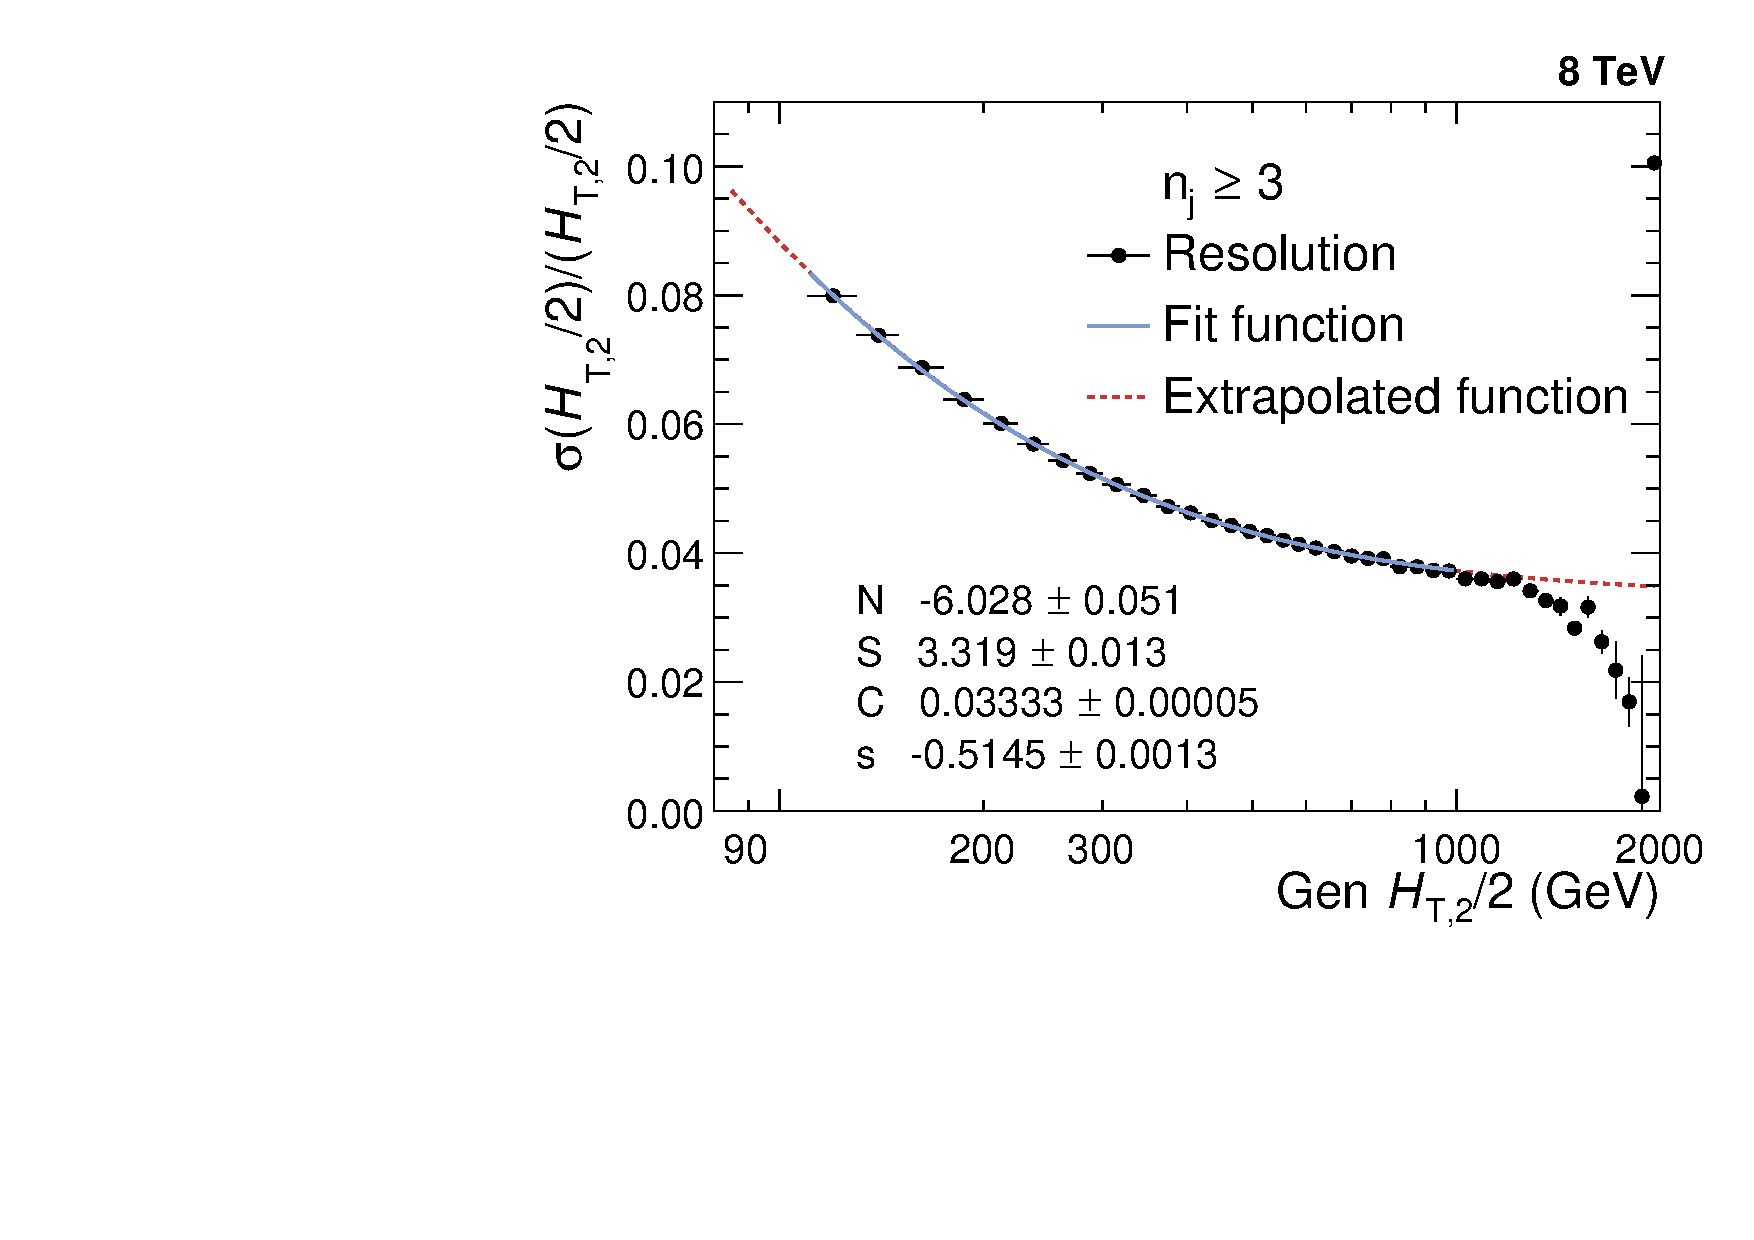
\includegraphics[scale = 0.215]{Plots_HT_2_150/Extrapolate_Sigma_Value_Res_3_crystal_ext.pdf}%
\includegraphics[scale = 0.215]{/home/anter/Desktop/Analysis_8/Present_Latex/After_Pre-approval/New_Plots_PAS/Comparison_Resolution_Crystal_32_divide.pdf}\\
\vspace{2mm}
\begin{center}
\begin{table}[htbp]
\centering\scriptsize
\begin{tabular}{ccccc}
        \hline \hline
                 &    N    &  S   &    C   &    s   \\ \hline
Inclusive 2-jet  & ~3.32 & 1.62 & 0.0333 & -0.318  \\
Inclusive 3-jet  & -6.03 & 3.32 & 0.0333 & -0.515  \\
\hline \hline 
\end{tabular}
\end{table}
\vspace{2mm}
\begin{itemize}
 {\scriptsize \item Resolution is similar in inclusive 3-jet and 2-jet (Right Fig.)
\vspace{2mm}
 \item Fit parameters are used for smearing of NLO spectrum to construct response matrices. \\ }
\end{itemize}
\end{center}
\end{frame}

%##################################### Slide : 41 ###########################################
\begin{frame}
\label{fit_formula1}
\frametitle{\centerline{Unfolding : Fitting NLO predictions}}
\setlength\labelsep {\dimexpr\labelsep + 0.05em\relax}
\setlength\leftmargini{\dimexpr\leftmargini + 0.05em\relax}
\vspace{-3mm}
\begin{center}
\begin{itemize}
\item {\tiny Fitting the NLO \httwot spectrum by the function \mycolor{(Function I)} \\}
\vspace{-7mm}
\begin{align*}
\resizebox{.38\hsize}{!}{$f(\httwo) = N (x_{T})^{-a} (1-x_{T})^{b} \times \exp(-c/x_{T})$}
\end{align*}
{\tiny where $N$ is normalization factor and $a$, $b$, $c$ are fit parameters.\\ }
\vspace{2mm}\tri
\begin{itemize}
\item {\tiny This function is derived from the below function from \textbf {``Measurement of the Inclusive Jet Cross Section in pp Collisions at $\sqrt{s}$=7 TeV'' (Phys.Rev.Lett. 107, 132001 (2011))}\\ }
\end{itemize}
\vspace{-2mm}
\begin{align*}
\resizebox{.58\hsize}{!}{$ f(p_{T};\alpha,\beta,\gamma) = N_{0} (p_{T})^{-\alpha}\bigg(1-\frac{2~p_{T}~cosh(y_{min})}{\sqrt{s}}\bigg)^{\beta} \times \exp(-\gamma/p_{T})$}
\end{align*}
\vspace{-5mm}
\begin{itemize}
\item[]{ \tiny using \\ }
\end{itemize}
\vspace{-5mm}
\begin{align*}
\resizebox{.6\hsize}{!}{${\alpha = a,~~\beta = b,~~\gamma = c*\sqrt{s}/2},~~{x_{T} = \frac{2*\httwotns*cosh(y_{min})}{\sqrt{s}}} = \frac{2*\httwot}{\sqrt{s}}$}
\end{align*}
\begin{itemize}
\vspace{-5mm}
\item[] {\tiny where transverse scaling variable $x_{T}$ corresponds to the proton fractional momentum $x$ for dijets with rapidity $y$ = 0, \cme = 8000 GeV and $y_{min}$ is low-edge of the rapidity bin $y$ under consideration. (Here $y_{min}$ is taken equal to 0). \\}
\end{itemize}
\end{itemize}
\vspace{2mm}\ball
\begin{itemize}
{\tiny \item Fitting the NLO \httwot spectrum by the function \mycolor{(Function II)} (\textbf{CMS AN-12-223}) :
\begin{align*}
{f(\httwotns) = A_{0}\Big(1-\frac{\httwotns}{A_{6}}\Big)^{A_{7}} \times 10^{F(\httwotns)}}, {\rm where} ~~~{F(x) = \sum\limits_{i=1}^5 A_{i}\Big(log\big(\frac{x}{A_{6}}\big)\Big)^{i}}~~~~~~~~~~~~~~~
\end{align*}
where the parameter $A_{6}$ is fixed to $\frac{\sqrt{s}}{2cosh(y_{min})}$, where ${\sqrt{s}}$ = 8000 GeV and $y_{min}$ is the minimum rapidity. The other parameters are derived from the fitting.\\ }
\end{itemize}
\end{center}
\end{frame}

%##################################### Slide : 13 ###########################################
\begin{frame}
\label{fit_formula2}
\frametitle{\centerline{Unfolding : Fitting NLO predictions}}
\setlength\labelsep {\dimexpr\labelsep + 0.05em\relax}
\setlength\leftmargini{\dimexpr\leftmargini + 0.05em\relax}
\vspace{-3mm}
\begin{center}
\begin{itemize}
\item {\scriptsize First fit the NLO spectrum with function and then using the obtained fit parameters extrapolated it to lower value.\\}
\end{itemize}
{\scriptsize \textbf {\mycolor{Function I (Left) and Function II (Right)}}}\\
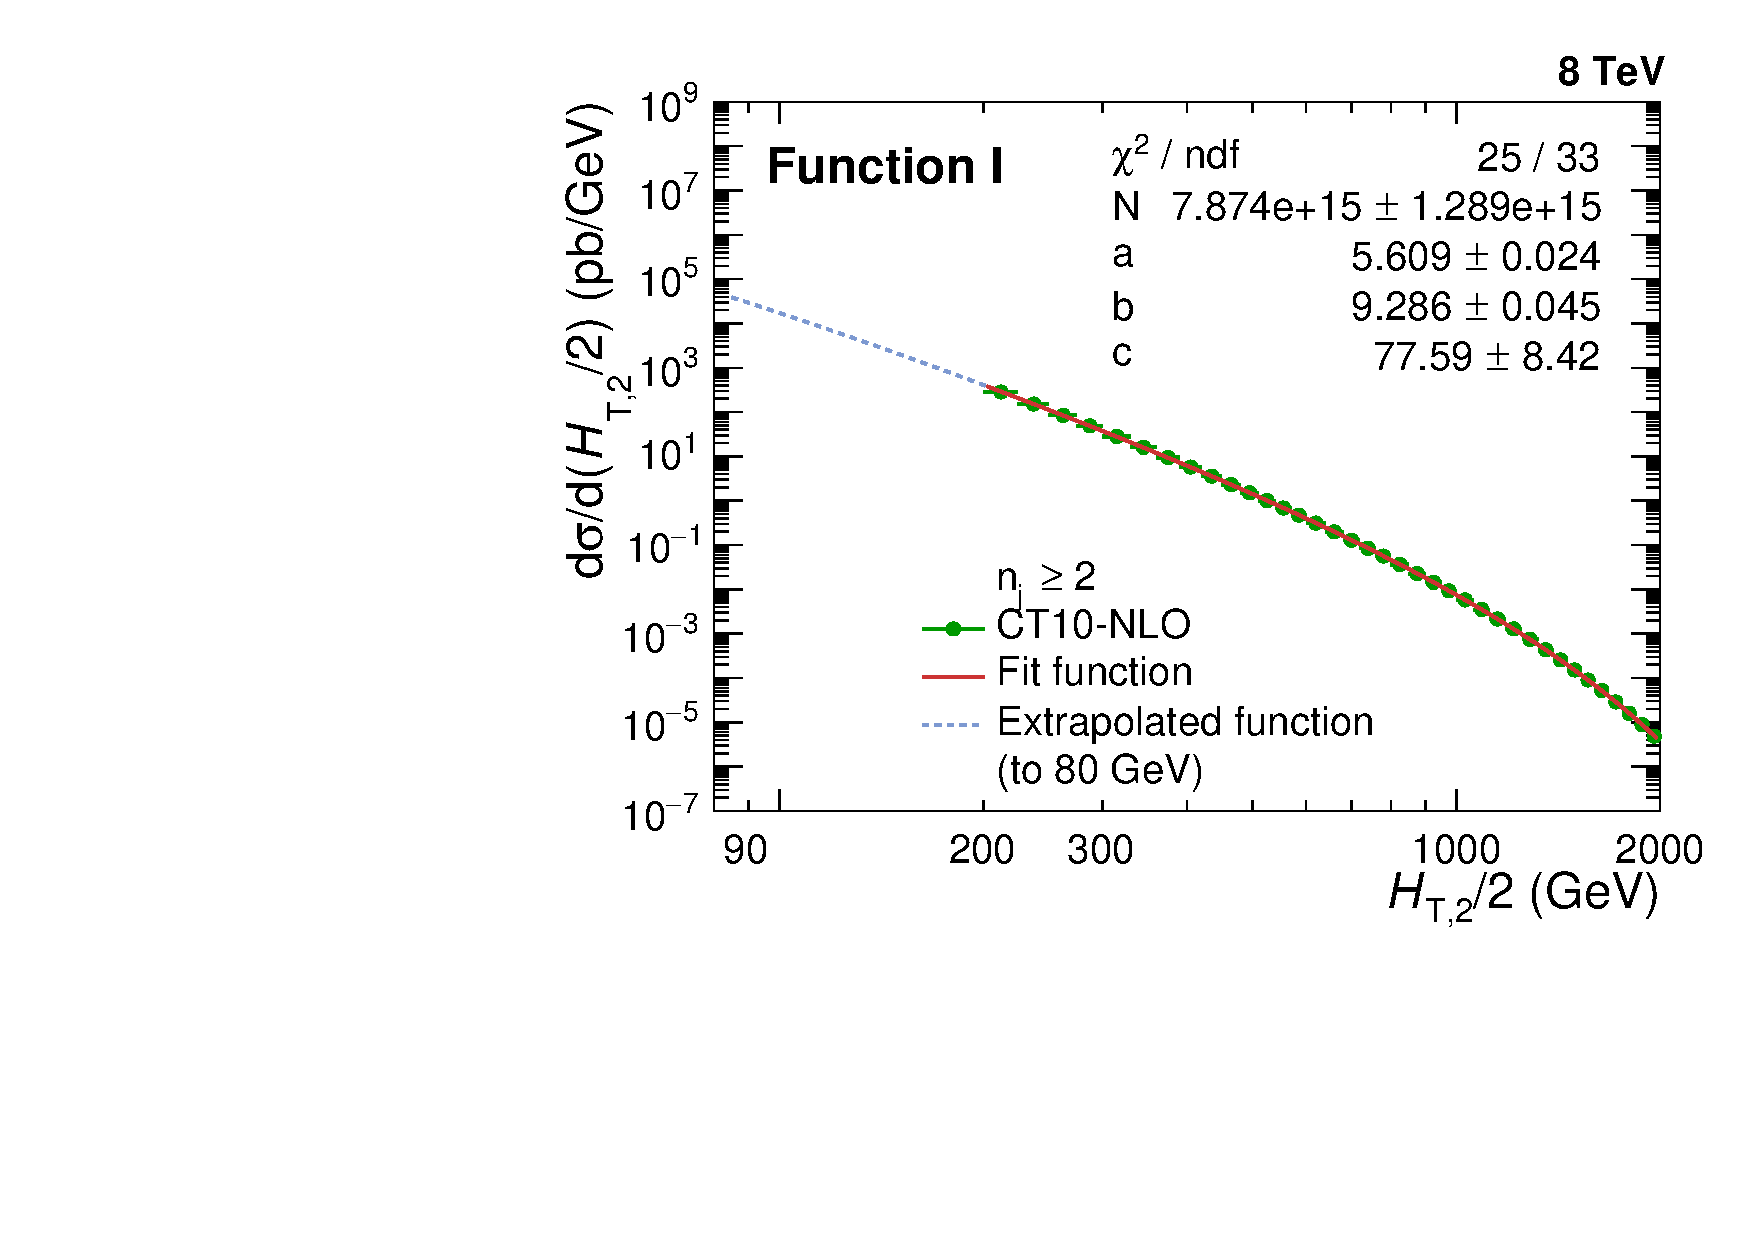
\includegraphics[scale = 0.22]{Plots_HT_2_150/Extrapolate_Theory_2_HT_2_150_funcI.pdf}%
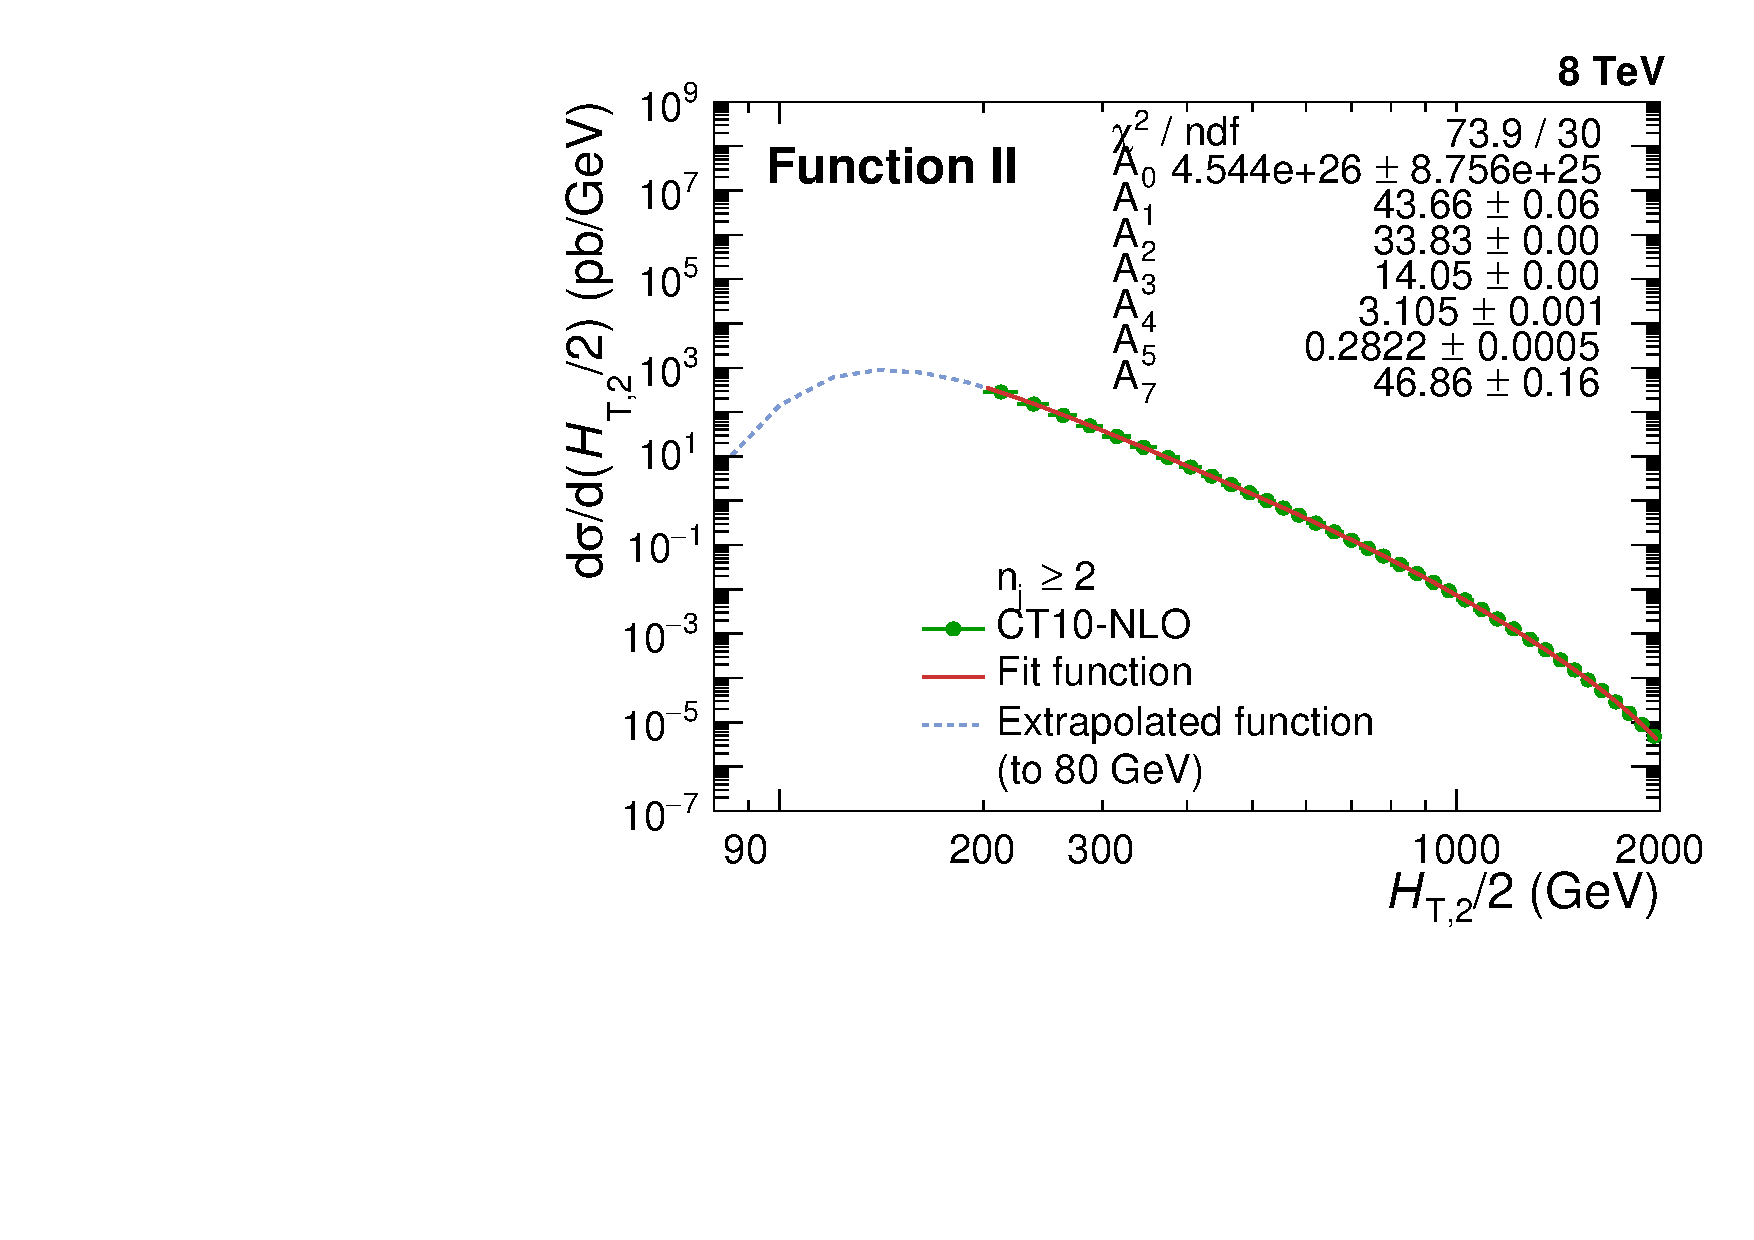
\includegraphics[scale = 0.22]{Plots_HT_2_150/Extrapolate_Theory_2_HT_2_150_funcII.pdf}\\
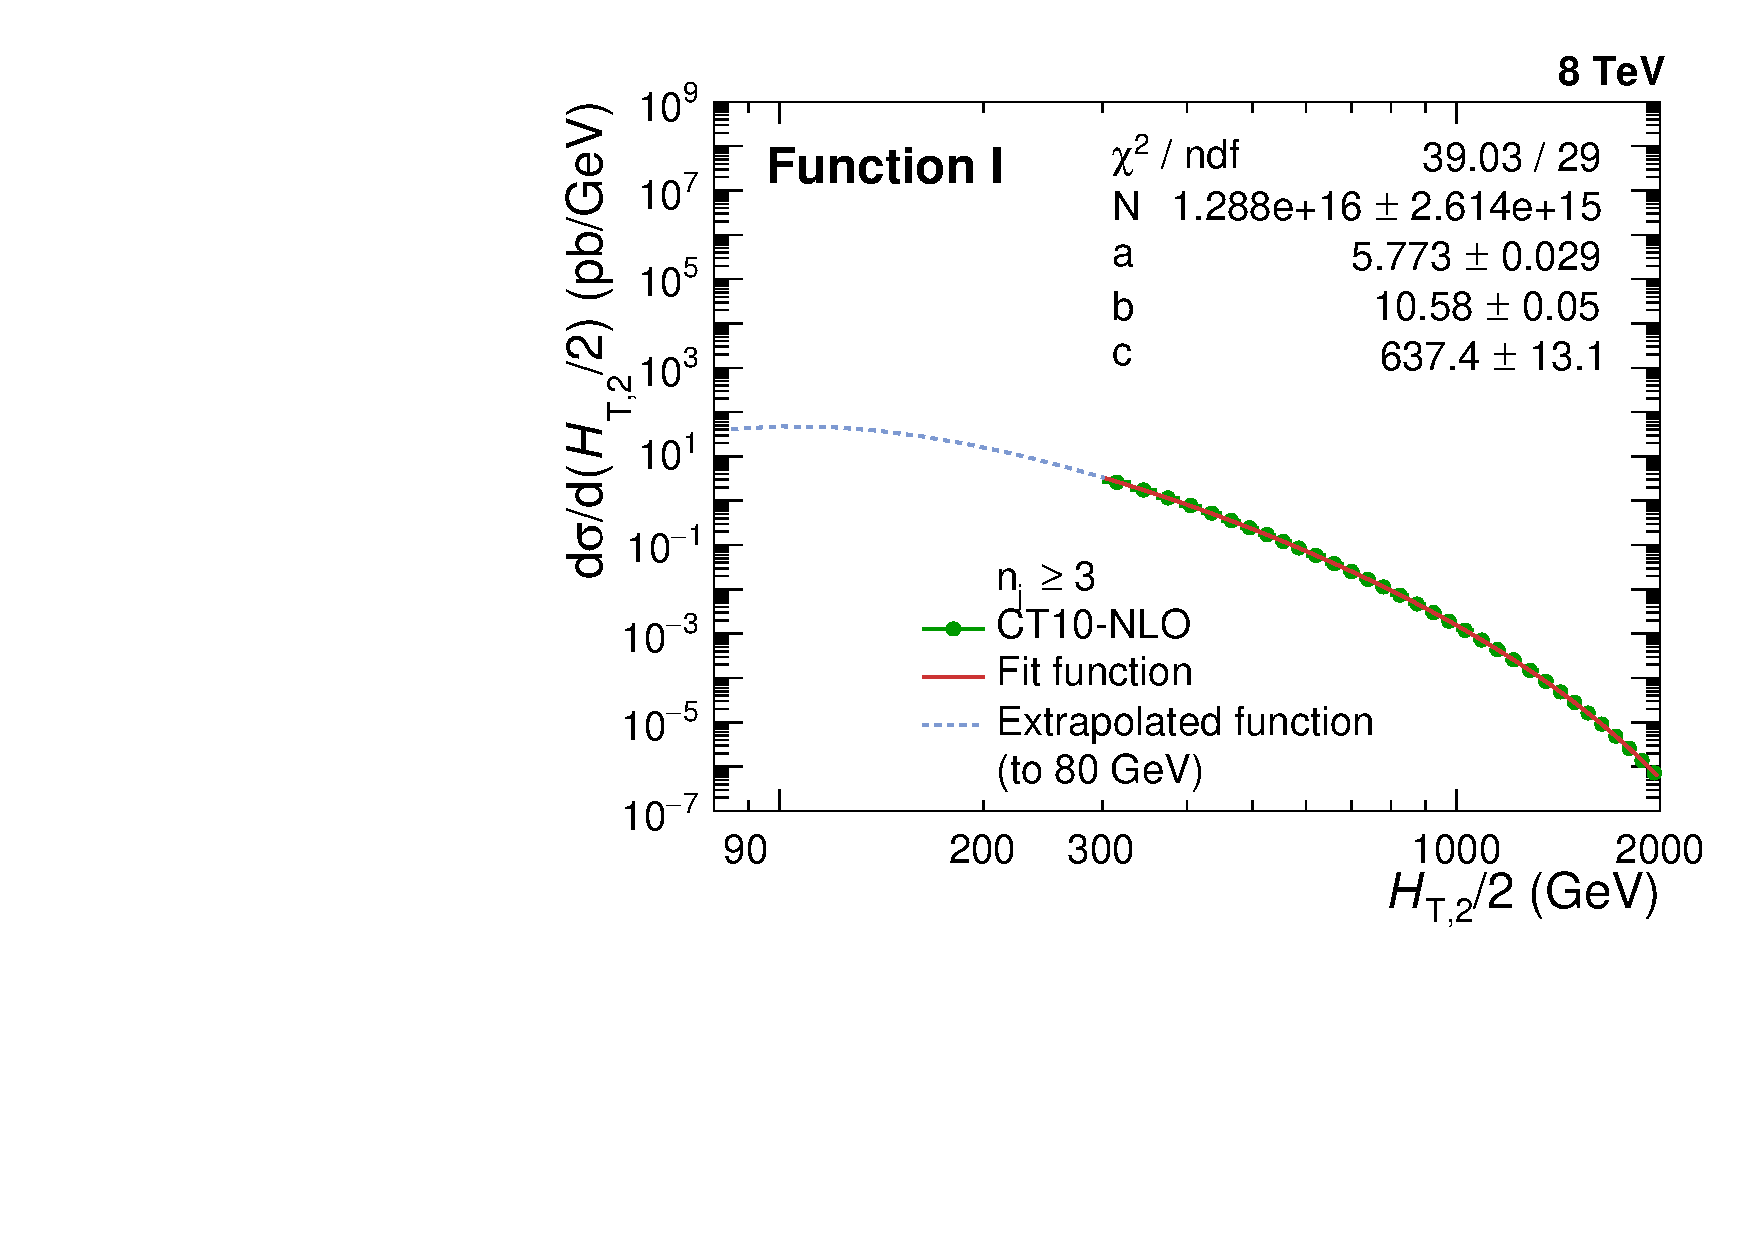
\includegraphics[scale = 0.22]{Plots_HT_2_150/Extrapolate_Theory_3_HT_2_150_funcI.pdf}%
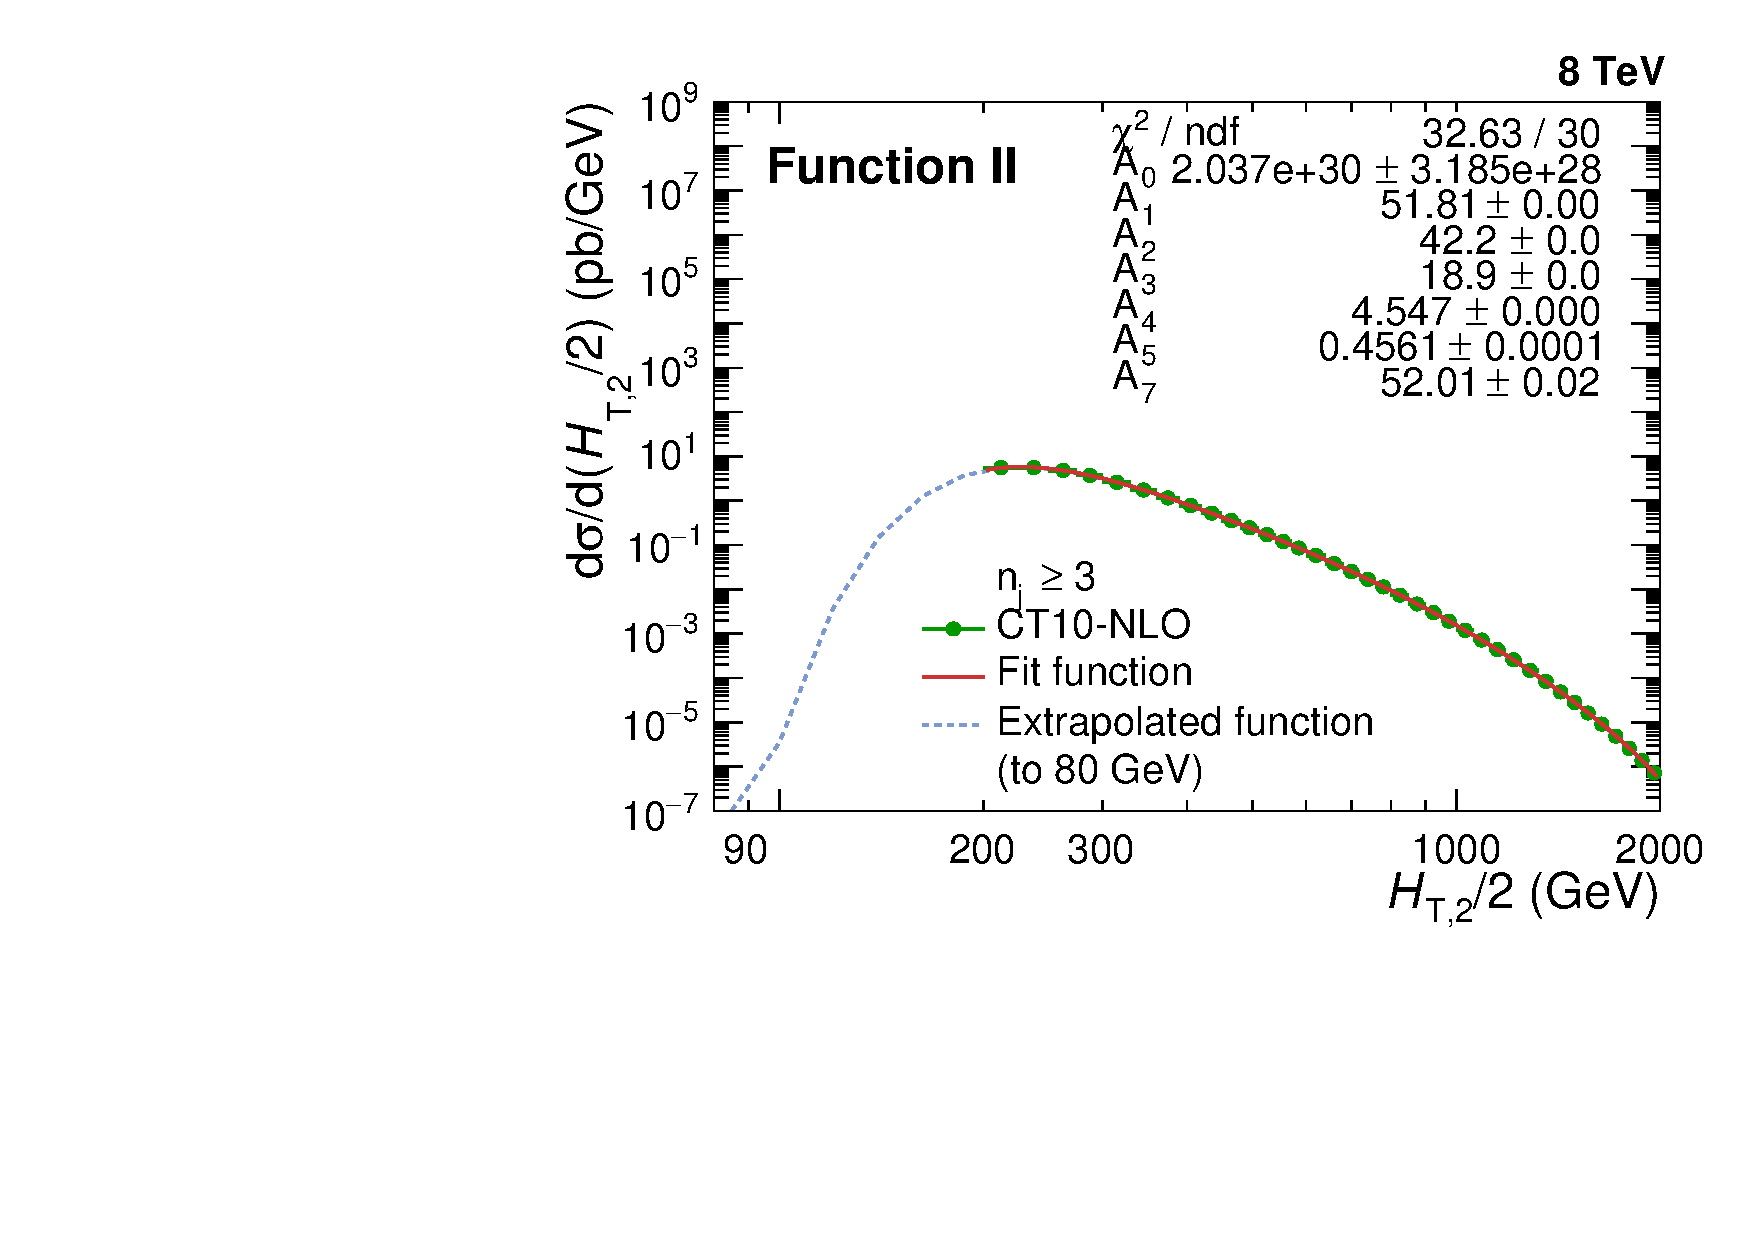
\includegraphics[scale = 0.22]{Plots_HT_2_150/Extrapolate_Theory_3_HT_2_150_funcII.pdf}
\end{center}
\end{frame}

%\item {\scriptsize Closure tests : small non-closures observed, accounted for additional uncertainity \\ (more details in Back-up slide no. \ref{closure}) \\ }

%##################################### Slide : 20 ###########################################
\begin{frame}
\label{theory_unc}
\frametitle{\centerline{Theoretical Uncertainties (CT14)}}
\setlength\labelsep {\dimexpr\labelsep + 0.05em\relax}
\setlength\leftmarginiii{\dimexpr\leftmarginiii + 0.05em\relax}
\vspace{-2mm}
\begin{center}
\includegraphics[scale = 0.26]{/home/anter/Desktop/Analysis_8/Present_Latex/Approval/Approval_New/Theory_Unc_2_CT14.pdf}%
\includegraphics[scale = 0.26]{/home/anter/Desktop/Analysis_8/Present_Latex/Approval/Approval_New/Theory_Unc_3_CT14.pdf}\\
\includegraphics[scale = 0.26]{/home/anter/Desktop/Analysis_8/Present_Latex/Approval/Approval_New/Theory_Unc_Ratio_32_CT14.pdf}\\
\end{center}
\end{frame}

%##################################### Slide : 25 ###########################################
\begin{frame}
\frametitle{\centerline{Sensitivity of differential inclusive 2-jet cross-section to \alpsmz}}
\setlength\labelsep {\dimexpr\labelsep + 0.05em\relax}
\setlength\leftmargini{\dimexpr\leftmargini + 0.05em\relax}
\begin{center}
\begin{itemize}
\item { \scriptsize $\rm {\sigma_{2\mbox{-}jet} \propto \alpsns^2}$ \\}
\end{itemize}
\vspace{5mm}
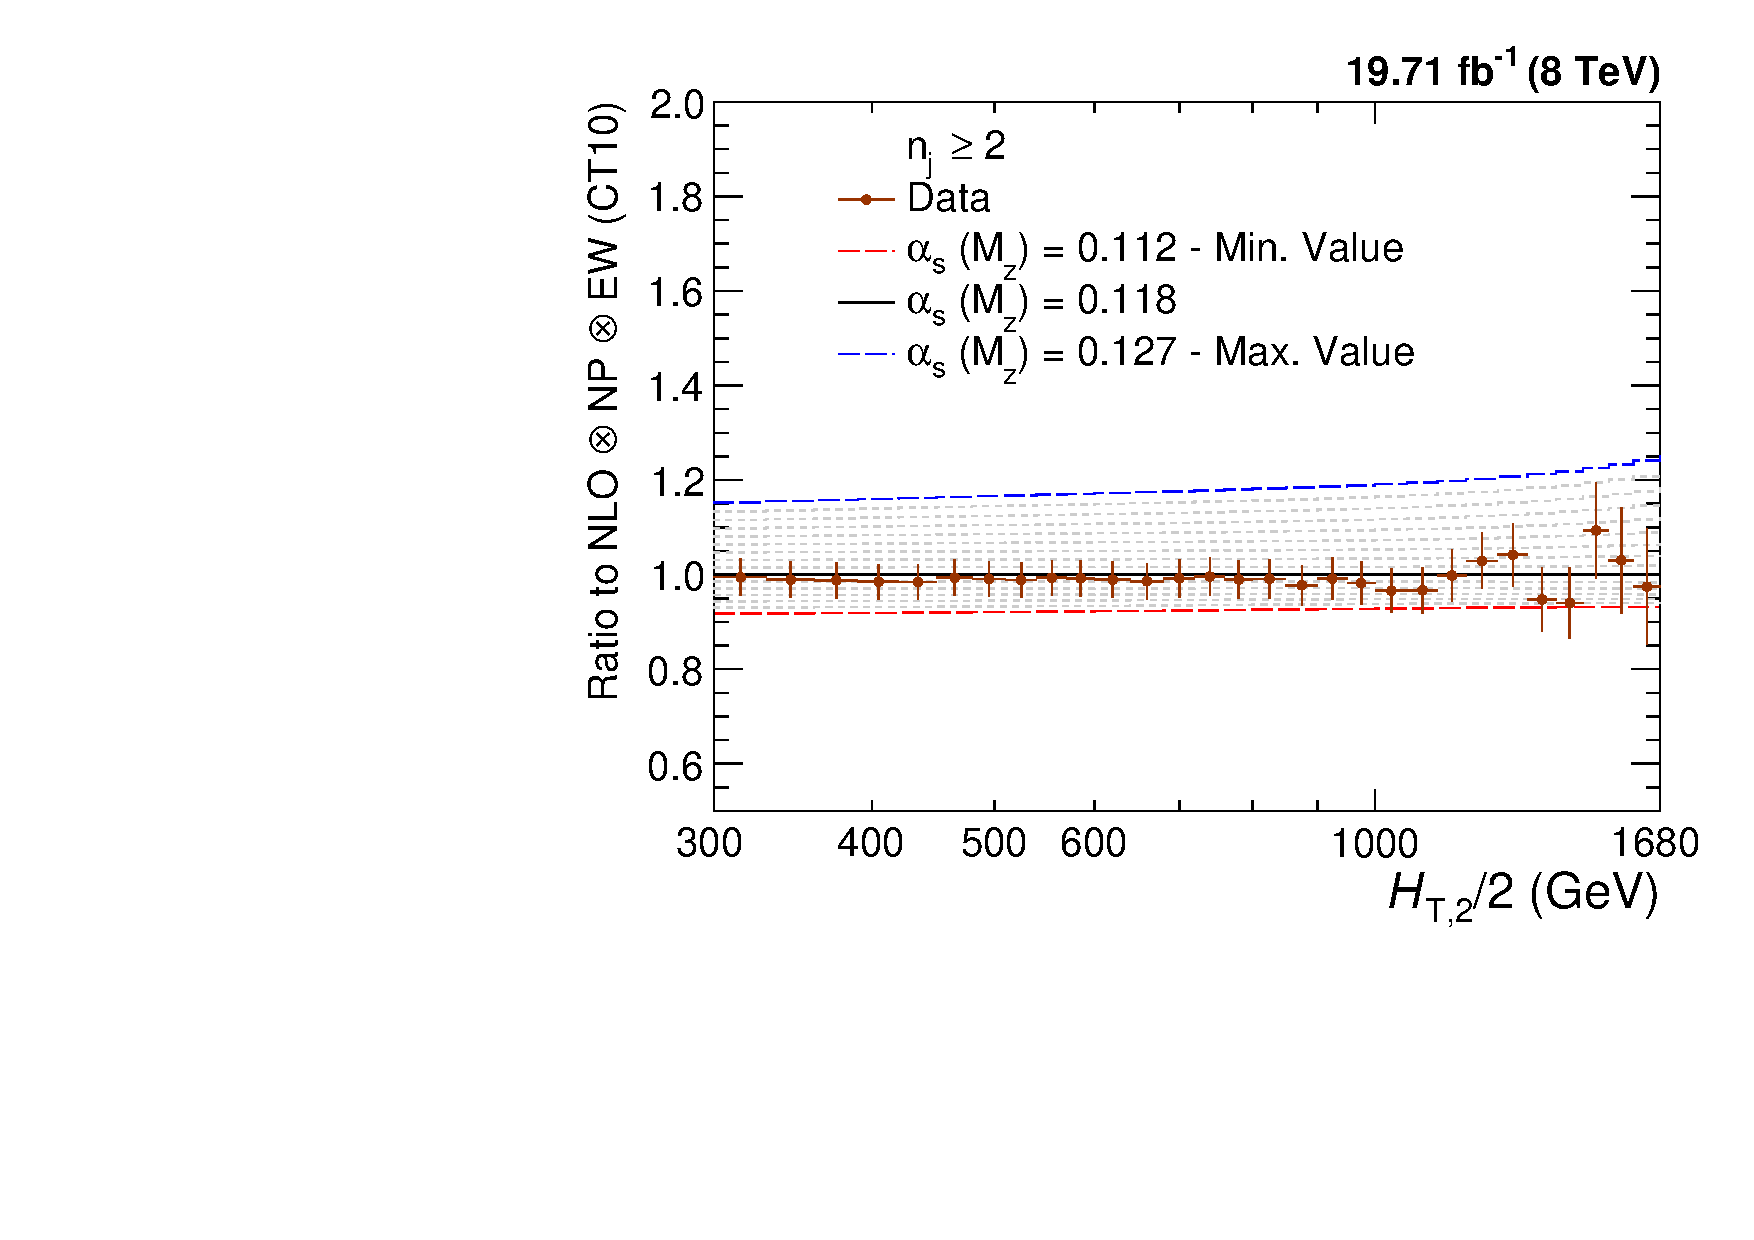
\includegraphics[scale = 0.207]{Plots_HT_2_150/Sensitivity_2_ratio_NLO_CT10_EW.pdf}%
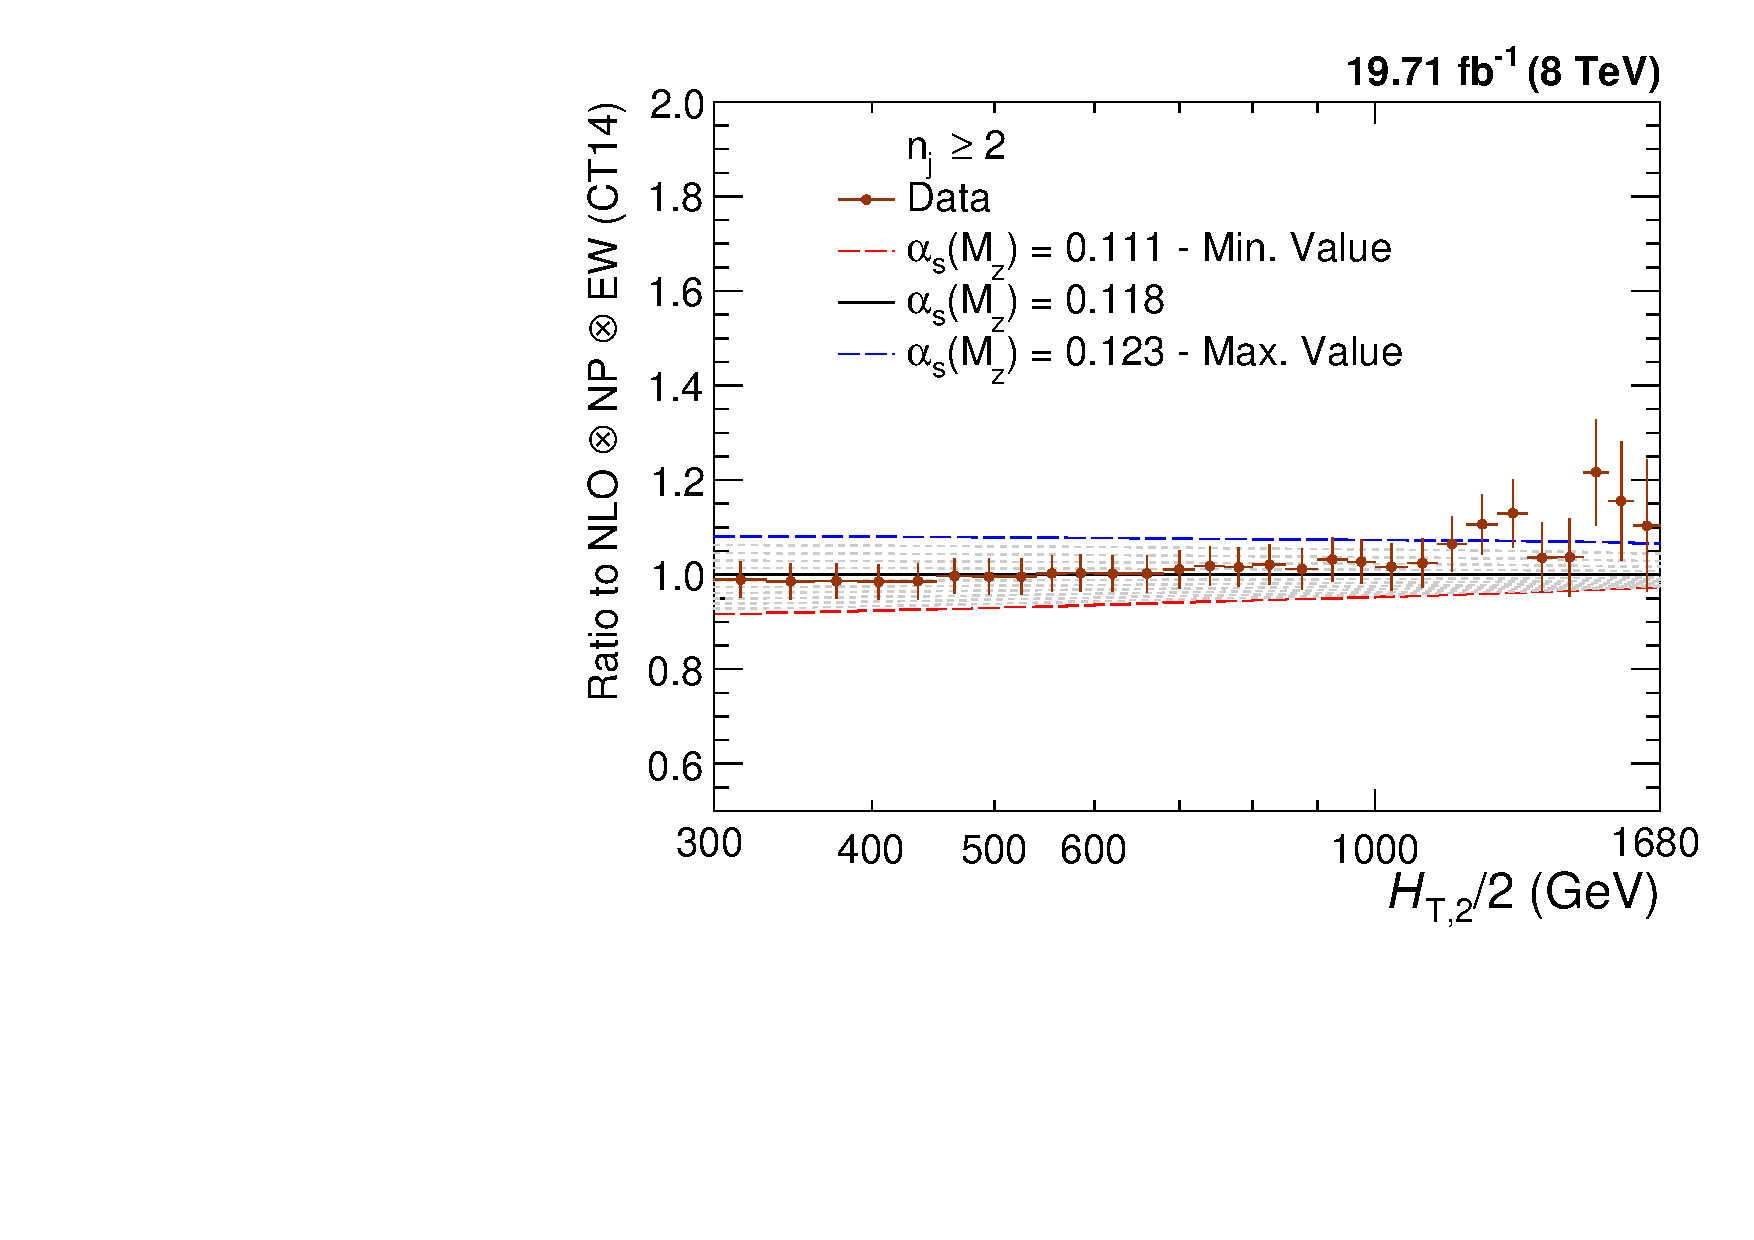
\includegraphics[scale = 0.207]{Plots_HT_2_150/Sensitivity_2_ratio_NLO_CT14_EW.pdf}%
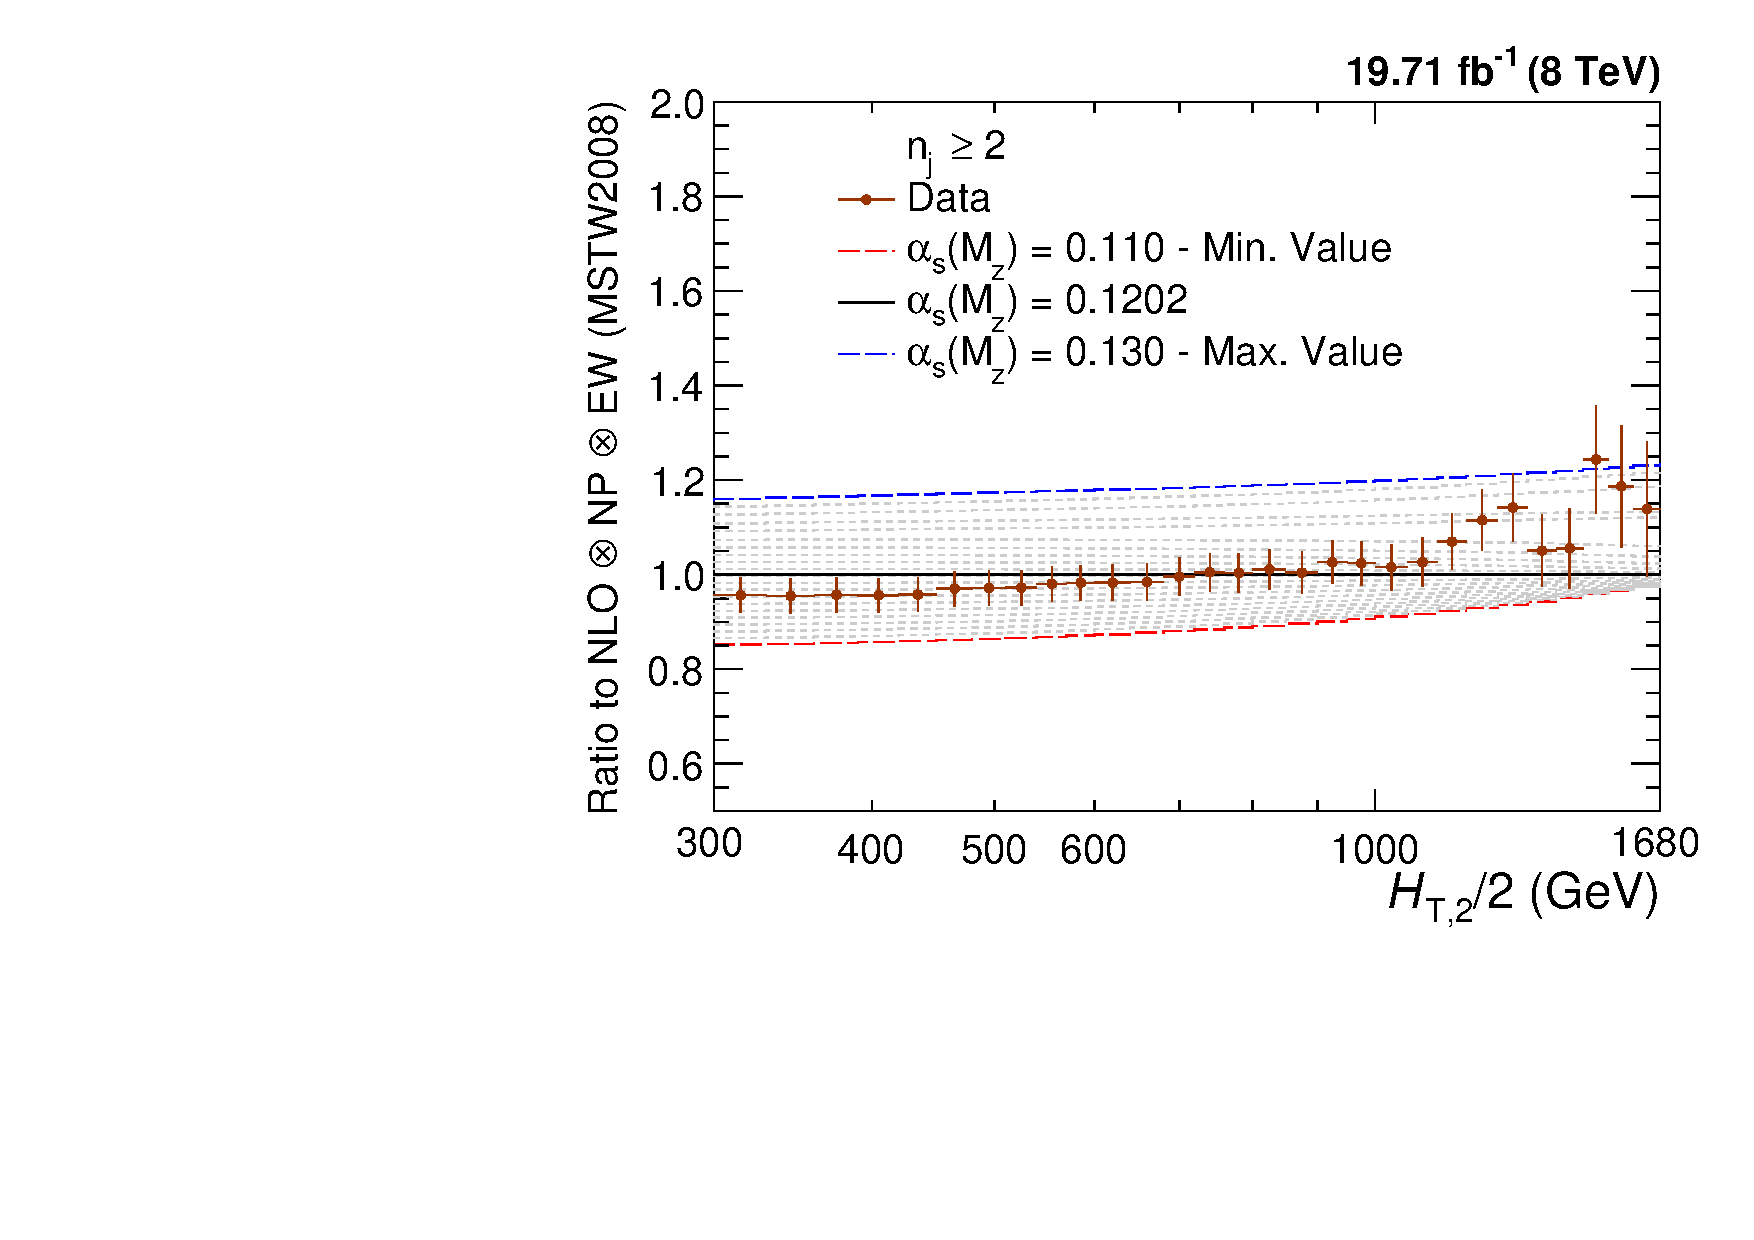
\includegraphics[scale = 0.207]{Plots_HT_2_150/Sensitivity_2_ratio_NLO_MSTW2008_EW.pdf}\\
\vspace{5mm}
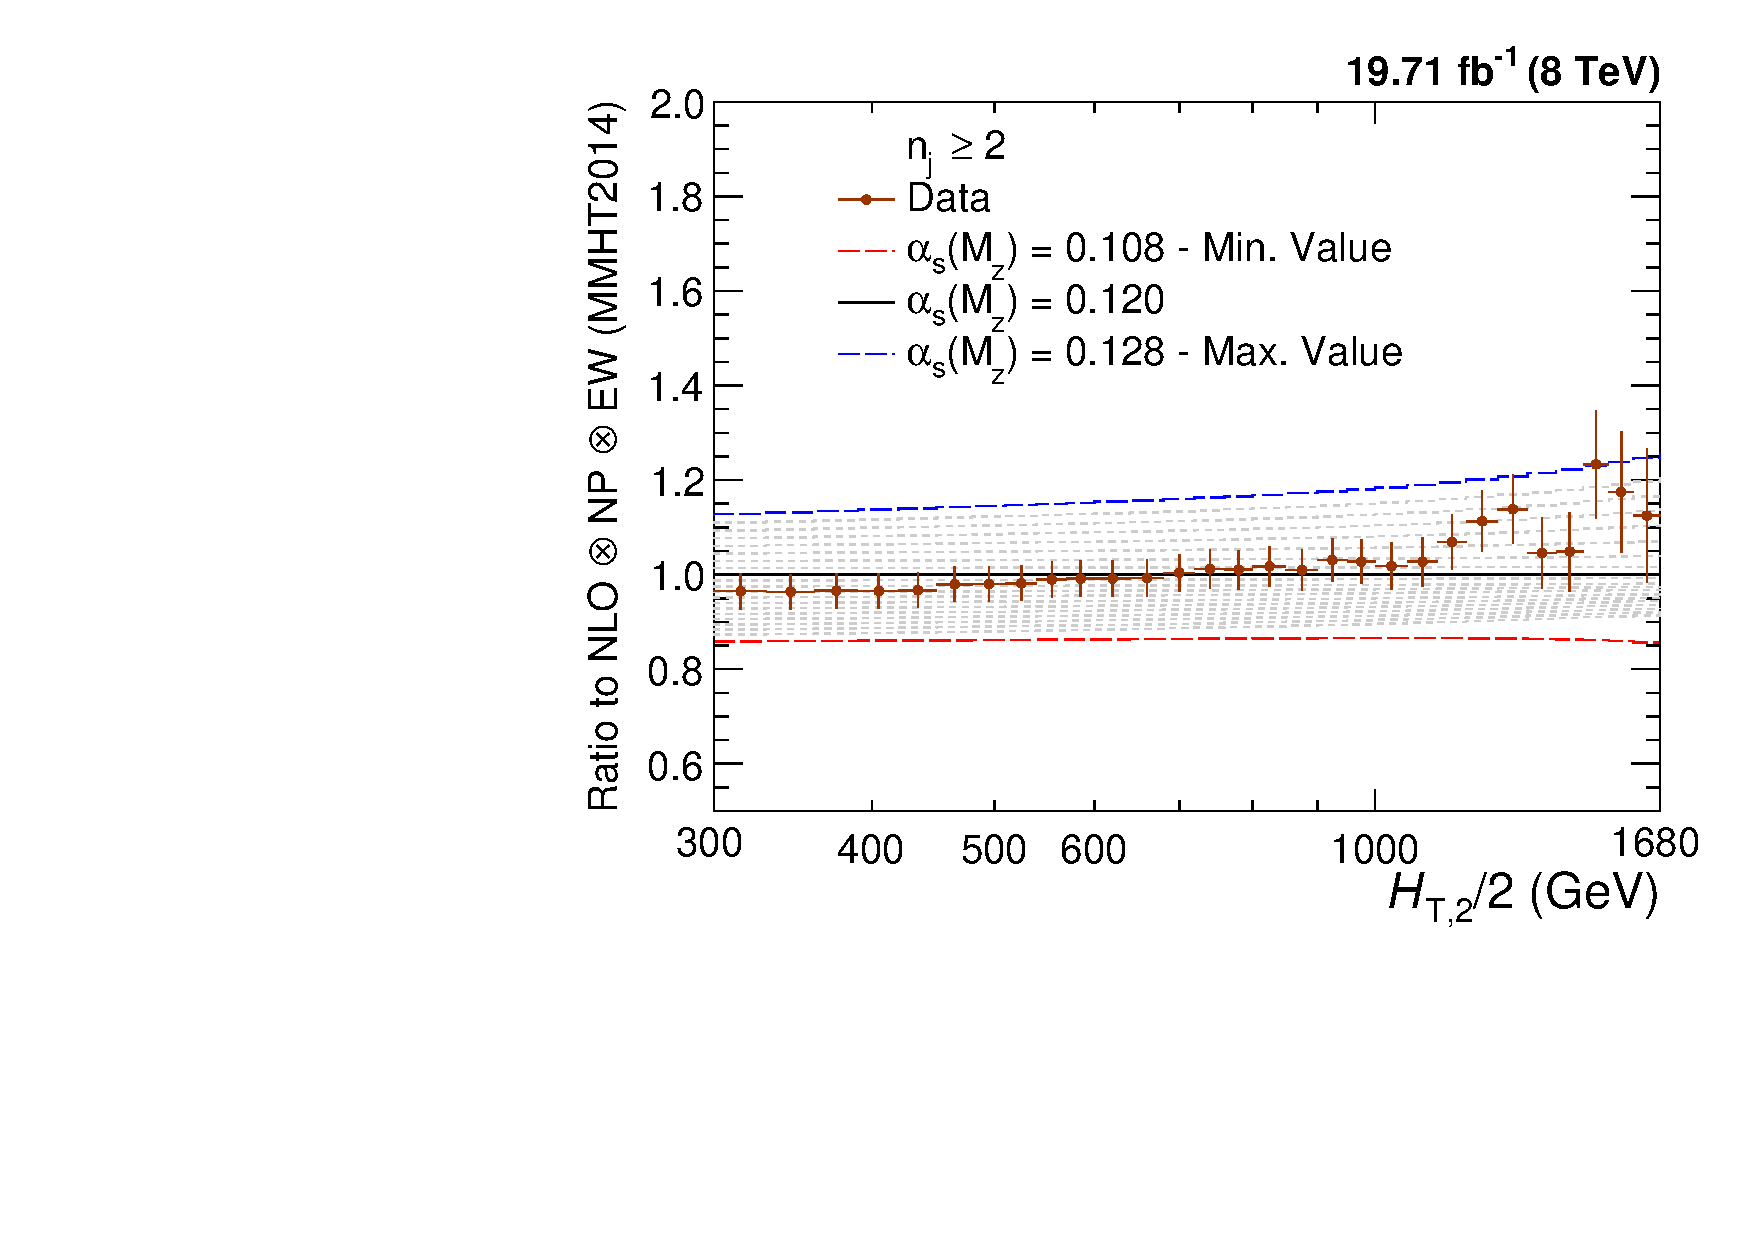
\includegraphics[scale = 0.207]{Plots_HT_2_150/Sensitivity_2_ratio_NLO_MMHT2014_EW.pdf}%
\hspace{0.3mm}
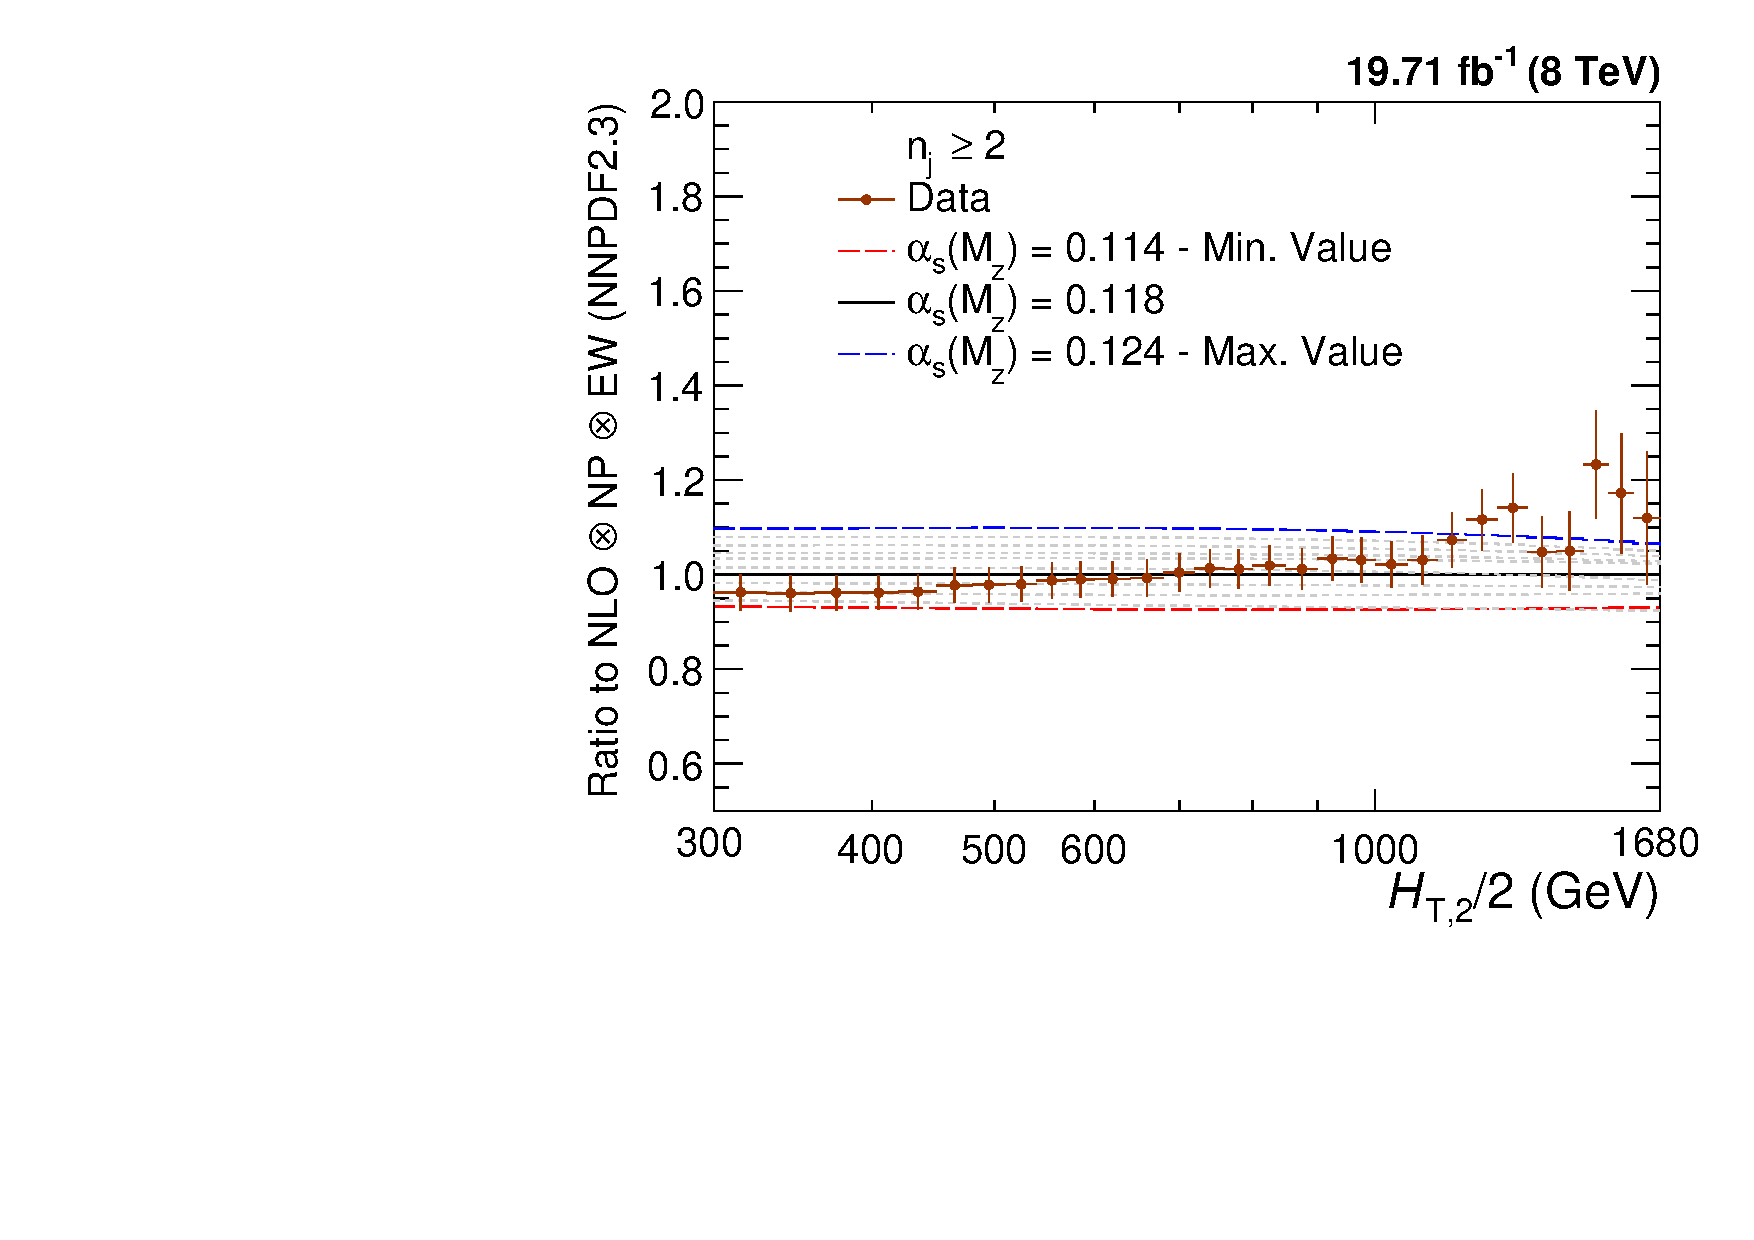
\includegraphics[scale = 0.207]{Plots_HT_2_150/Sensitivity_2_ratio_NLO_NNPDF23_EW.pdf}
\end{center}
\end{frame}

%##################################### Slide : 26 ###########################################
\begin{frame}
\frametitle{\centerline{Sensitivity of differential inclusive 3-jet cross-section to \alpsmz}}
\setlength\labelsep {\dimexpr\labelsep + 0.05em\relax}
\setlength\leftmargini{\dimexpr\leftmargini + 0.05em\relax}
\begin{center}
\begin{itemize}
\item { \scriptsize $\rm {\sigma_{3\mbox{-}jet} \propto \alpsns^3}$ \\}
\end{itemize}
\vspace{5mm}
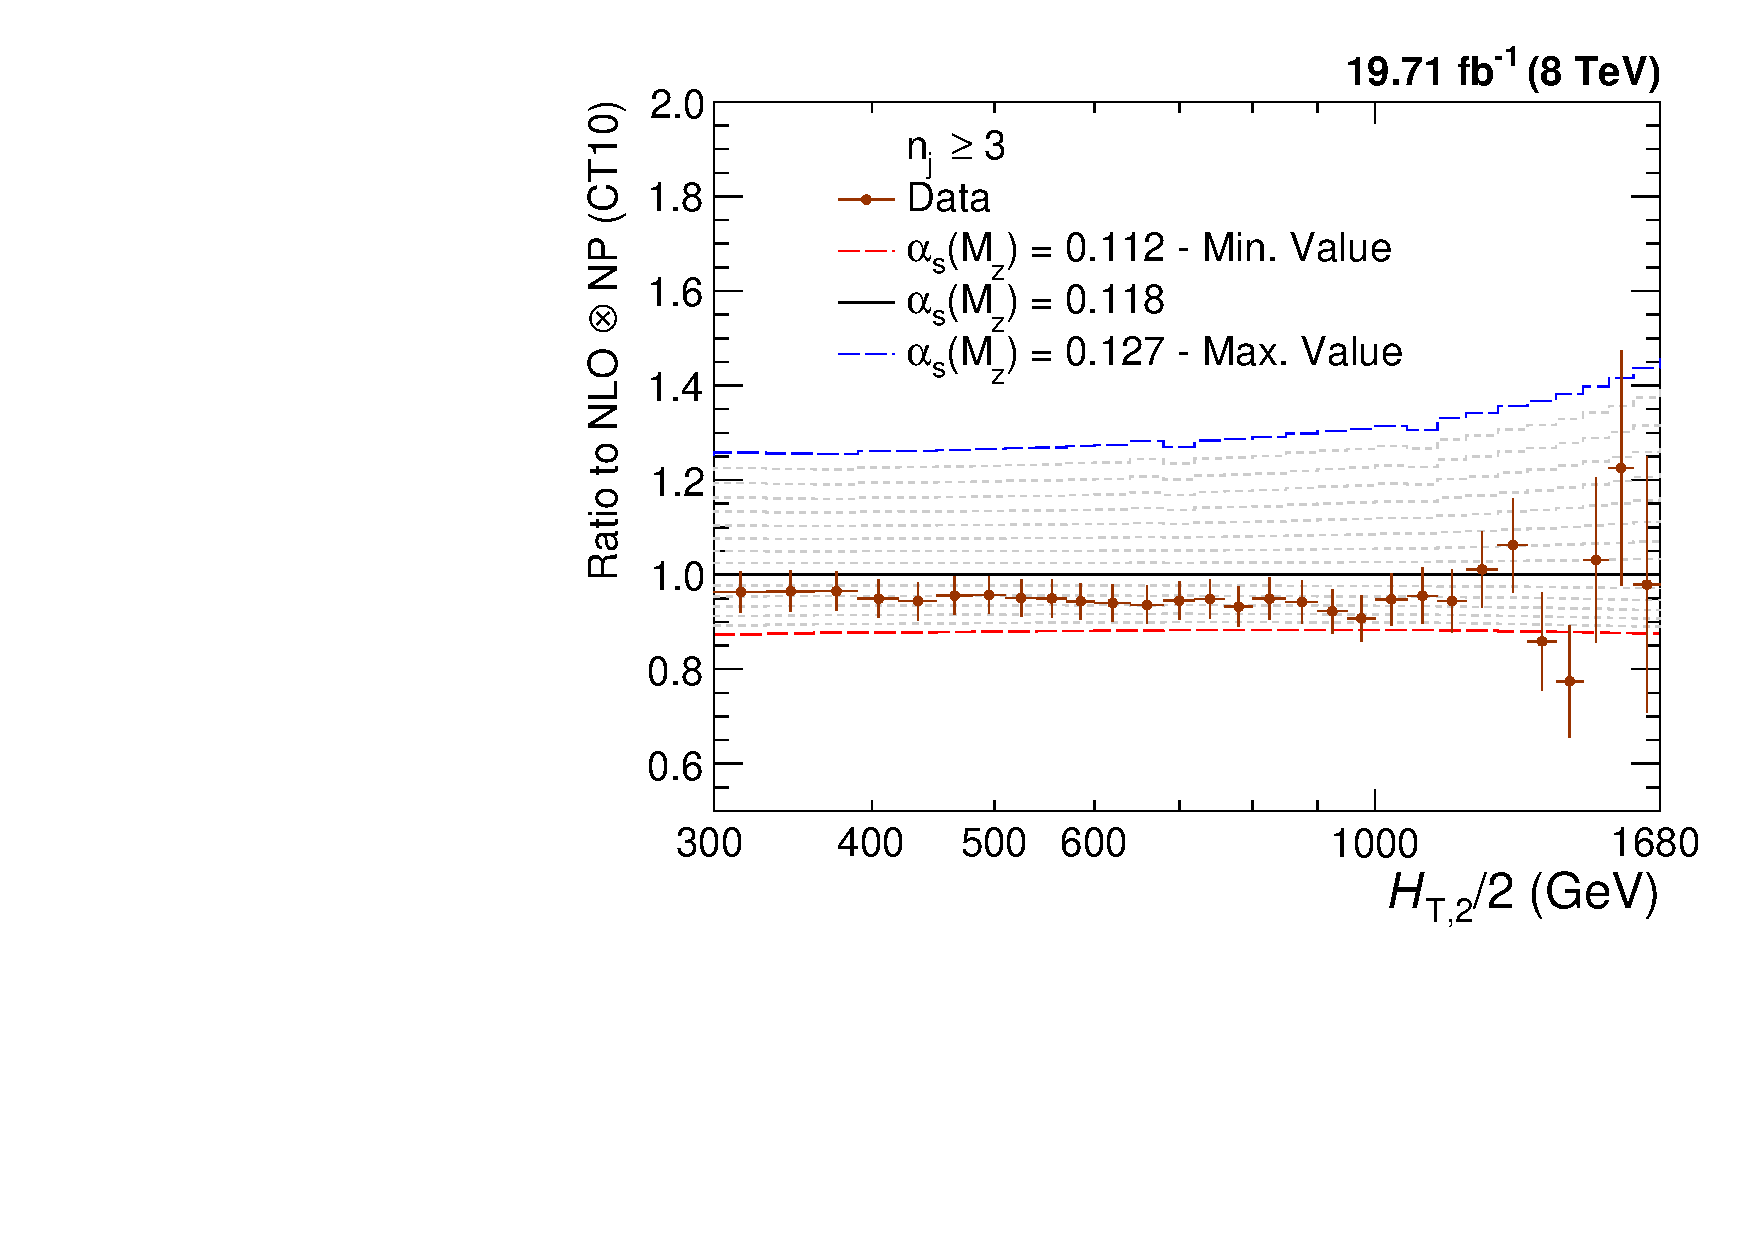
\includegraphics[scale = 0.207]{Plots_HT_2_150/Sensitivity_3_ratio_NLO_CT10.pdf}%
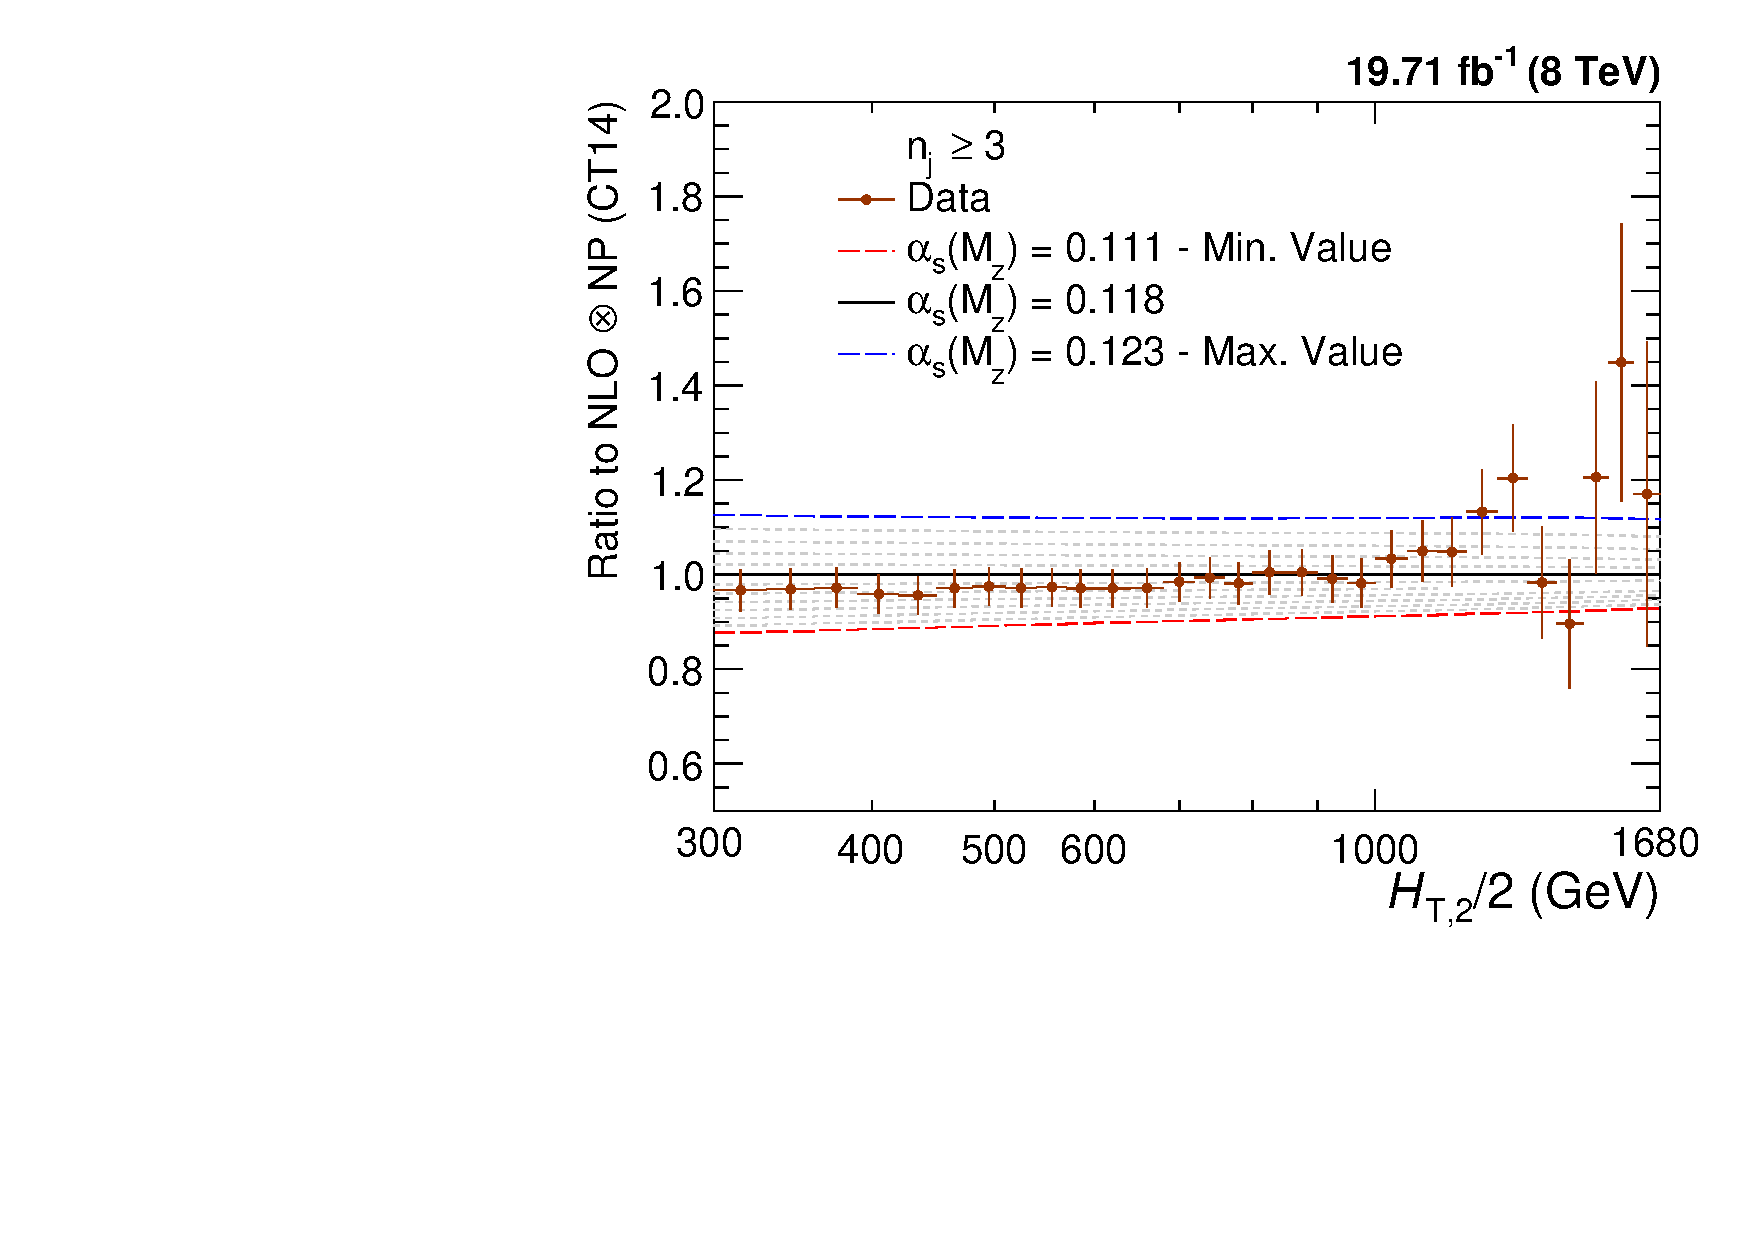
\includegraphics[scale = 0.207]{Plots_HT_2_150/Sensitivity_3_ratio_NLO_CT14.pdf}%
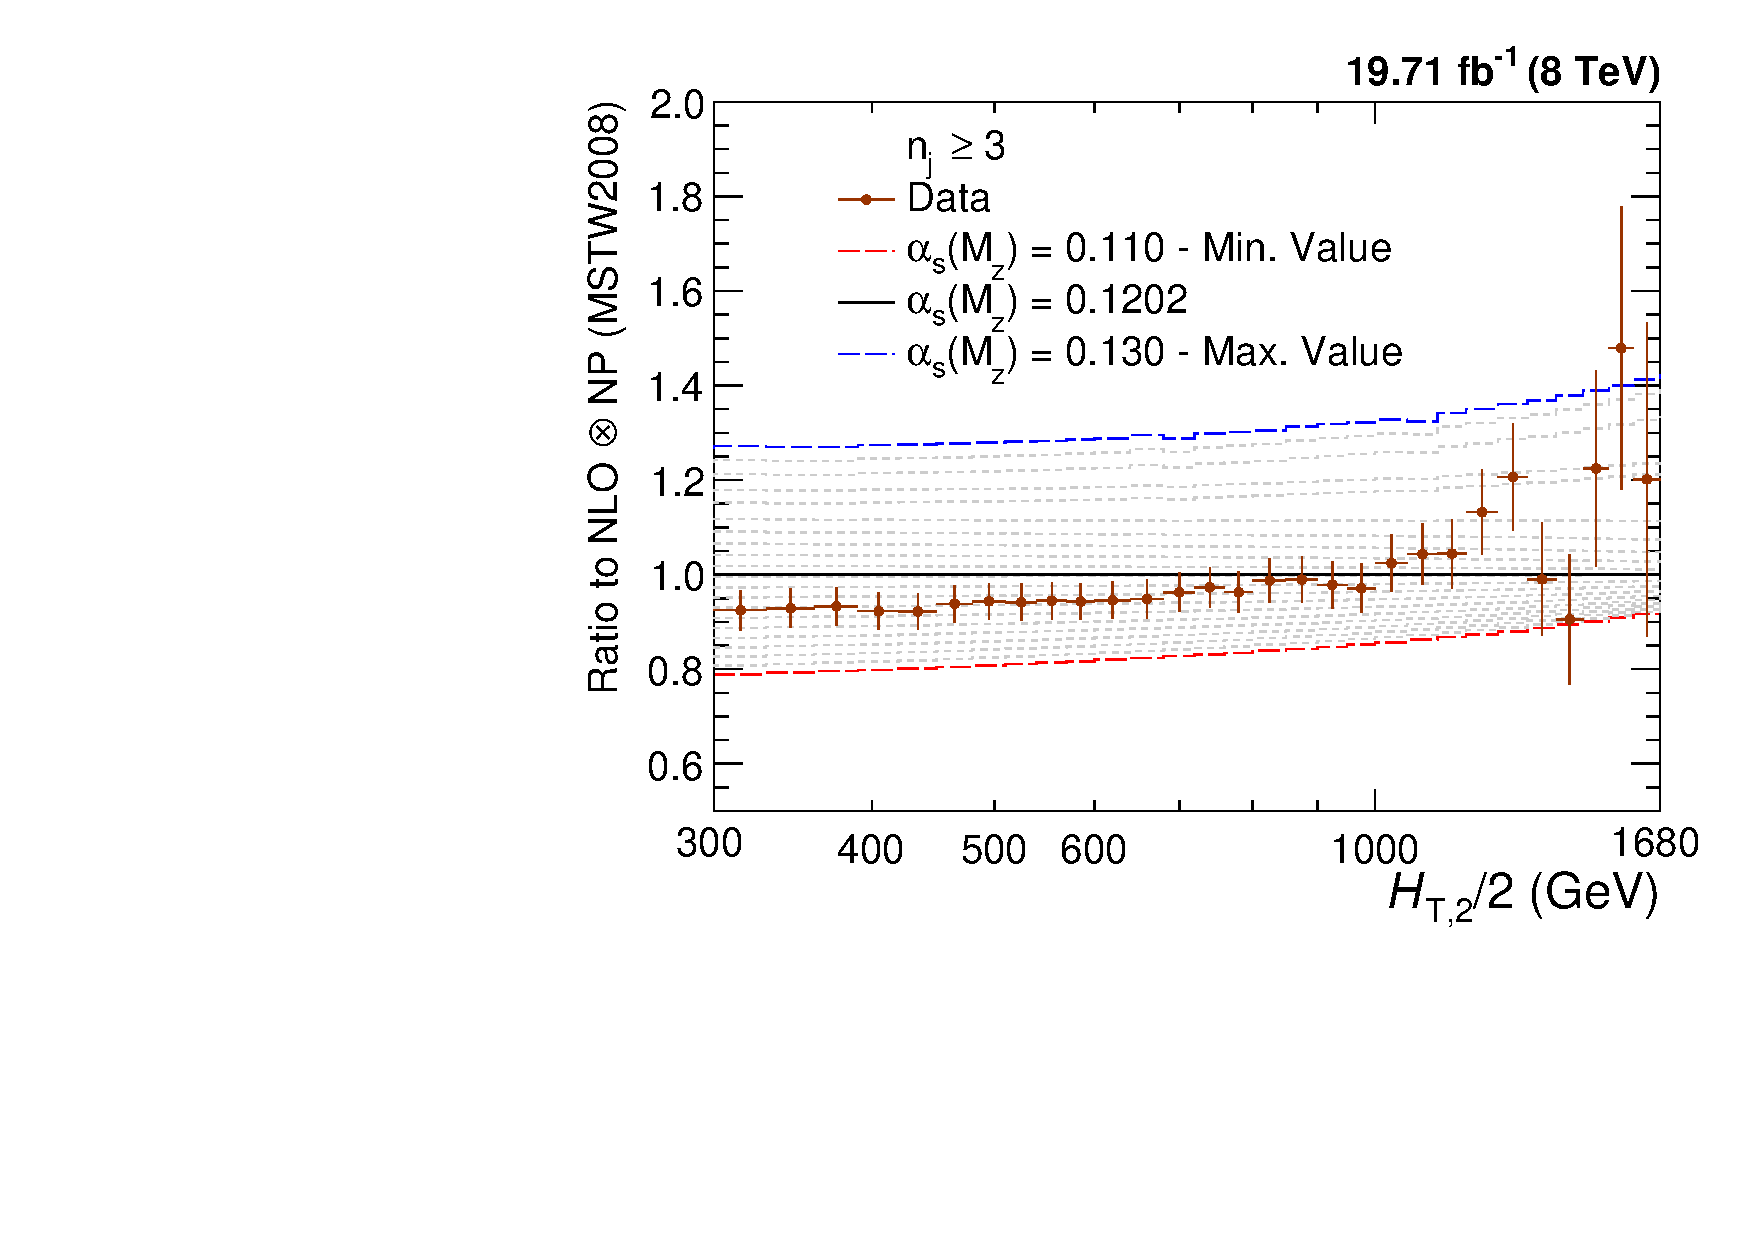
\includegraphics[scale = 0.207]{Plots_HT_2_150/Sensitivity_3_ratio_NLO_MSTW2008.pdf}\\
\vspace{5mm}
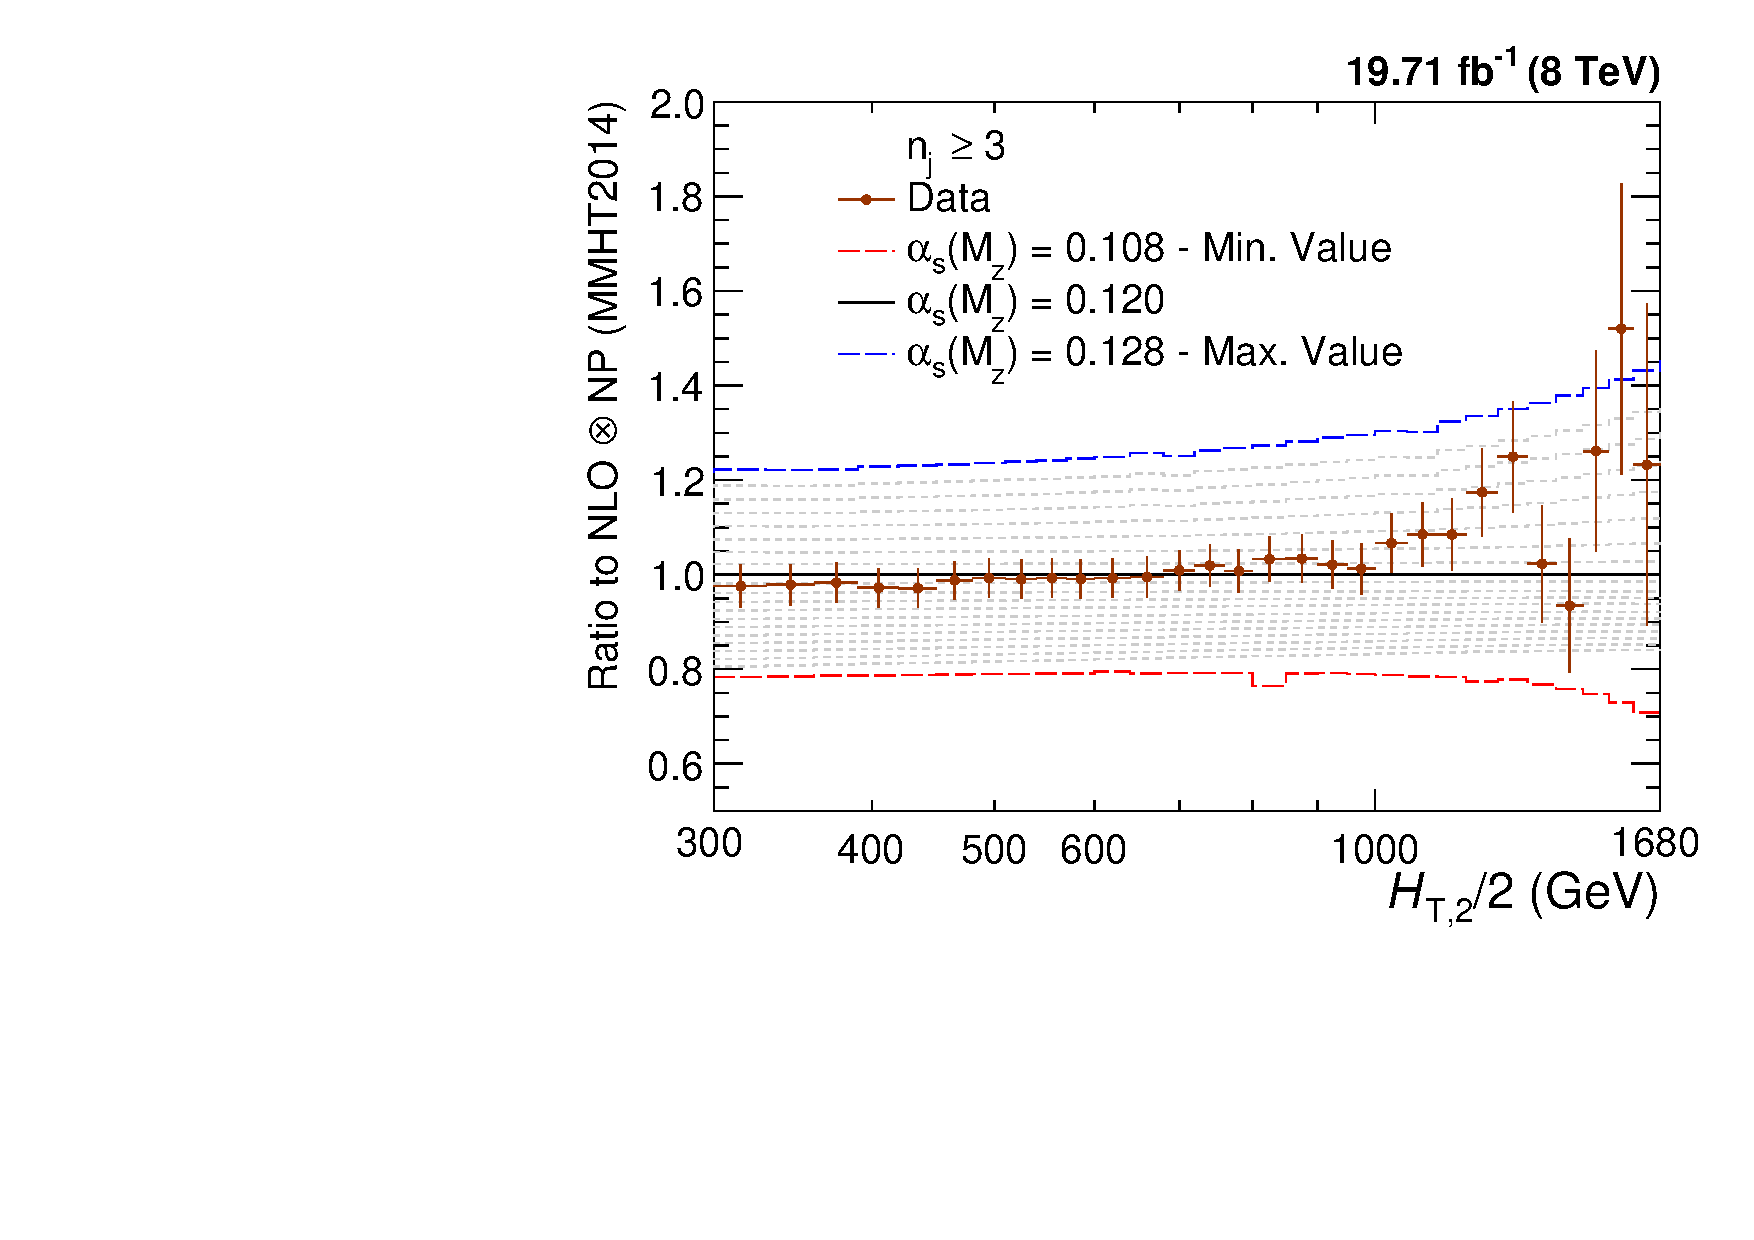
\includegraphics[scale = 0.207]{Plots_HT_2_150/Sensitivity_3_ratio_NLO_MMHT2014.pdf}%
\hspace{0.3mm}
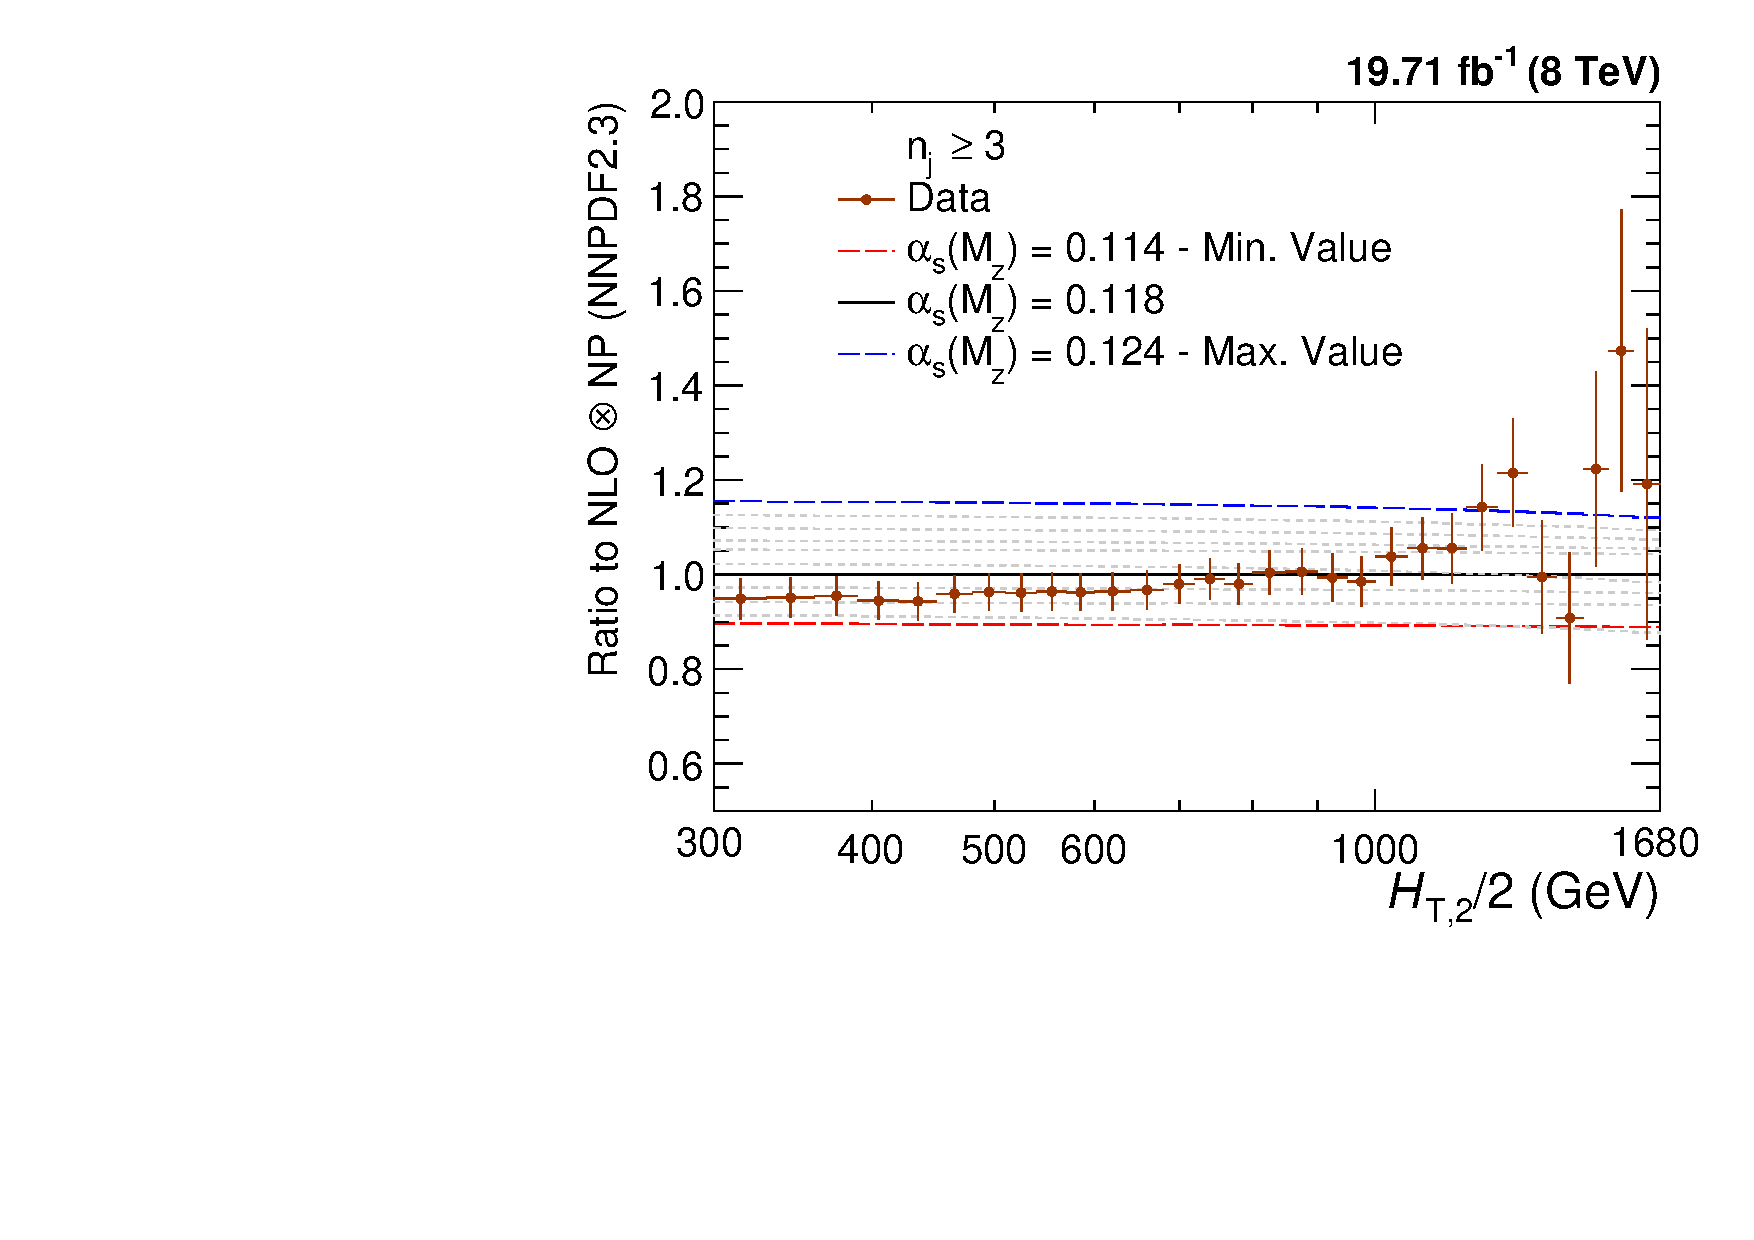
\includegraphics[scale = 0.207]{Plots_HT_2_150/Sensitivity_3_ratio_NLO_NNPDF23.pdf}
\end{center}
\end{frame}

%##################################### Slide : 27 ###########################################
\begin{frame}
\frametitle{\centerline{Sensitivity of \ratio to \alpsmz}}
\setlength\labelsep {\dimexpr\labelsep + 0.05em\relax}
\setlength\leftmargini{\dimexpr\leftmargini + 0.05em\relax}
\begin{center}
\begin{itemize}
\item {\scriptsize $\rm {\ratio \propto \alpsns^1}$ \\}
\end{itemize}
\vspace{5mm}
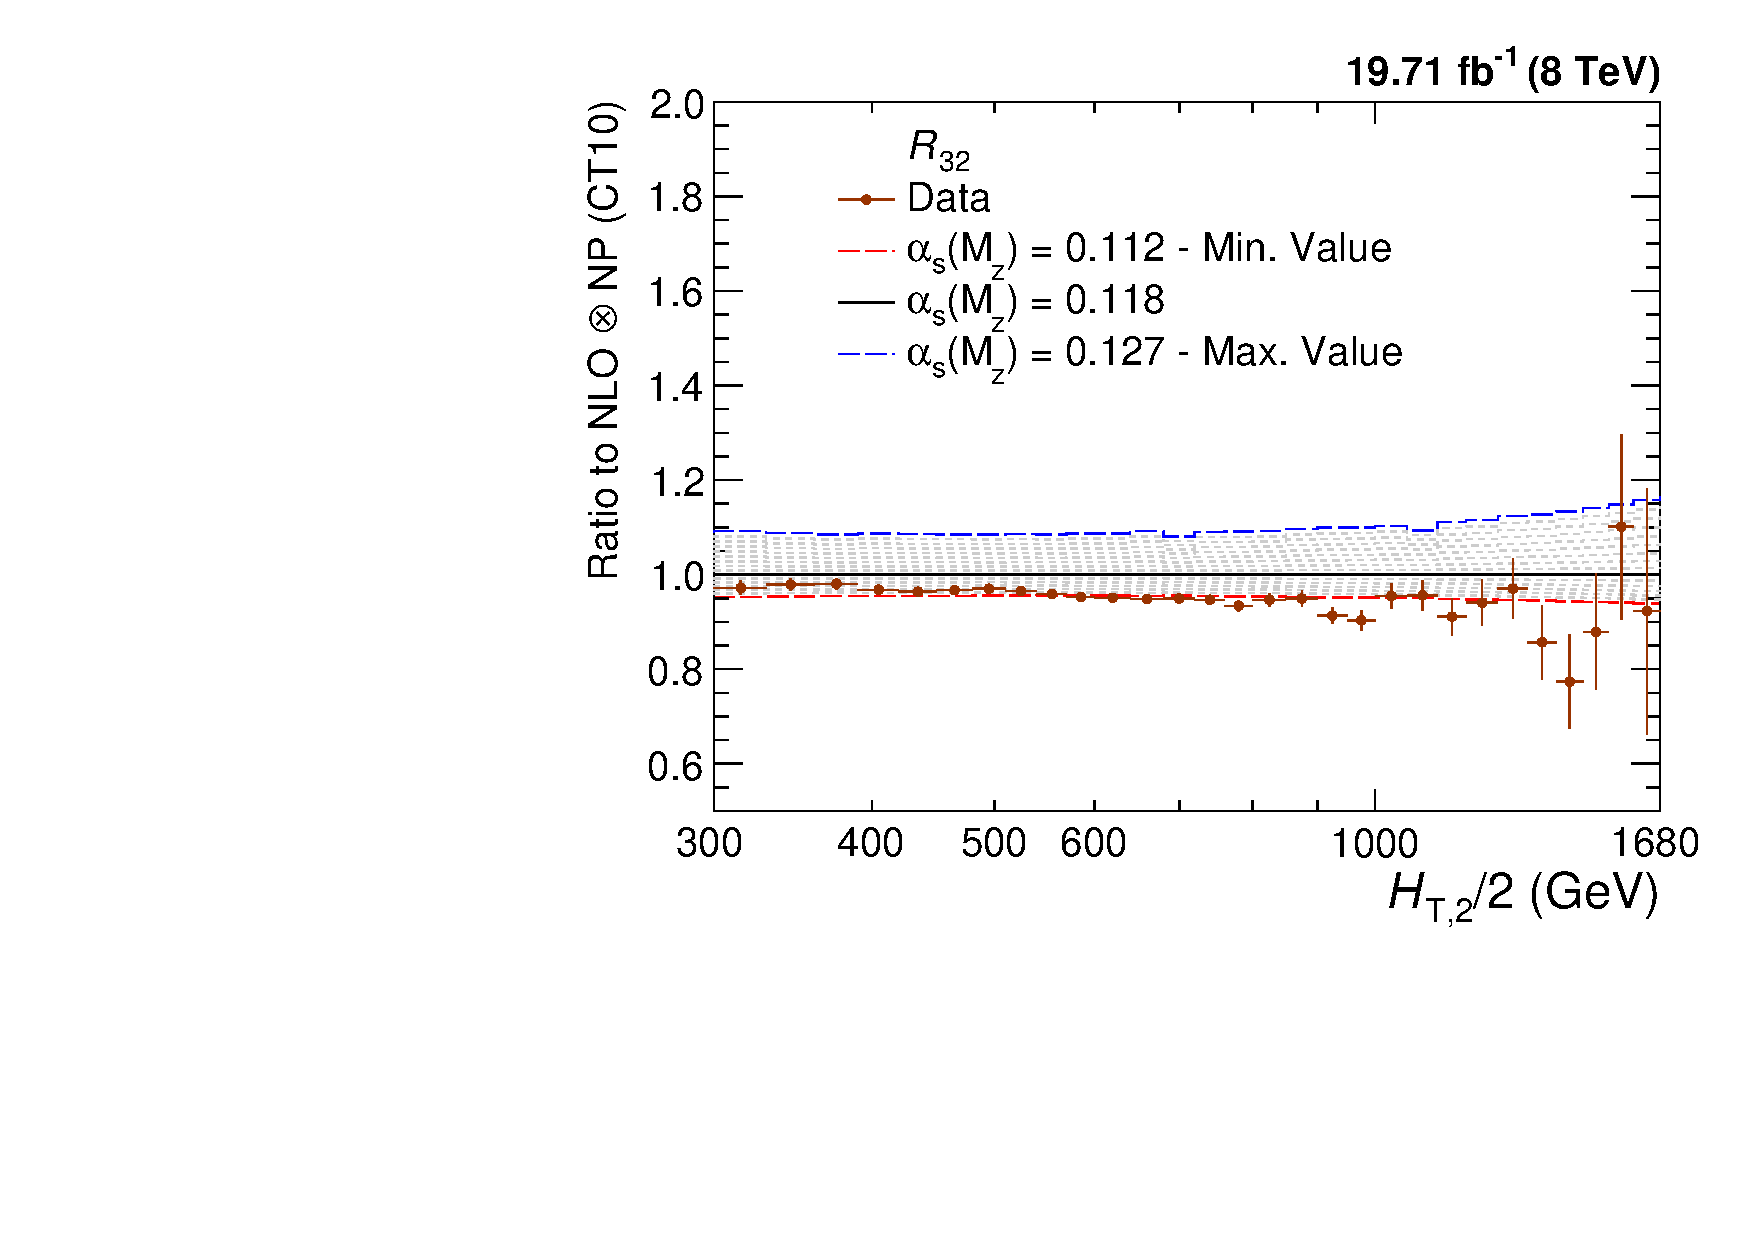
\includegraphics[scale = 0.207]{Plots_HT_2_150/Sensitivity_double_ratio_32_CT10.pdf}%
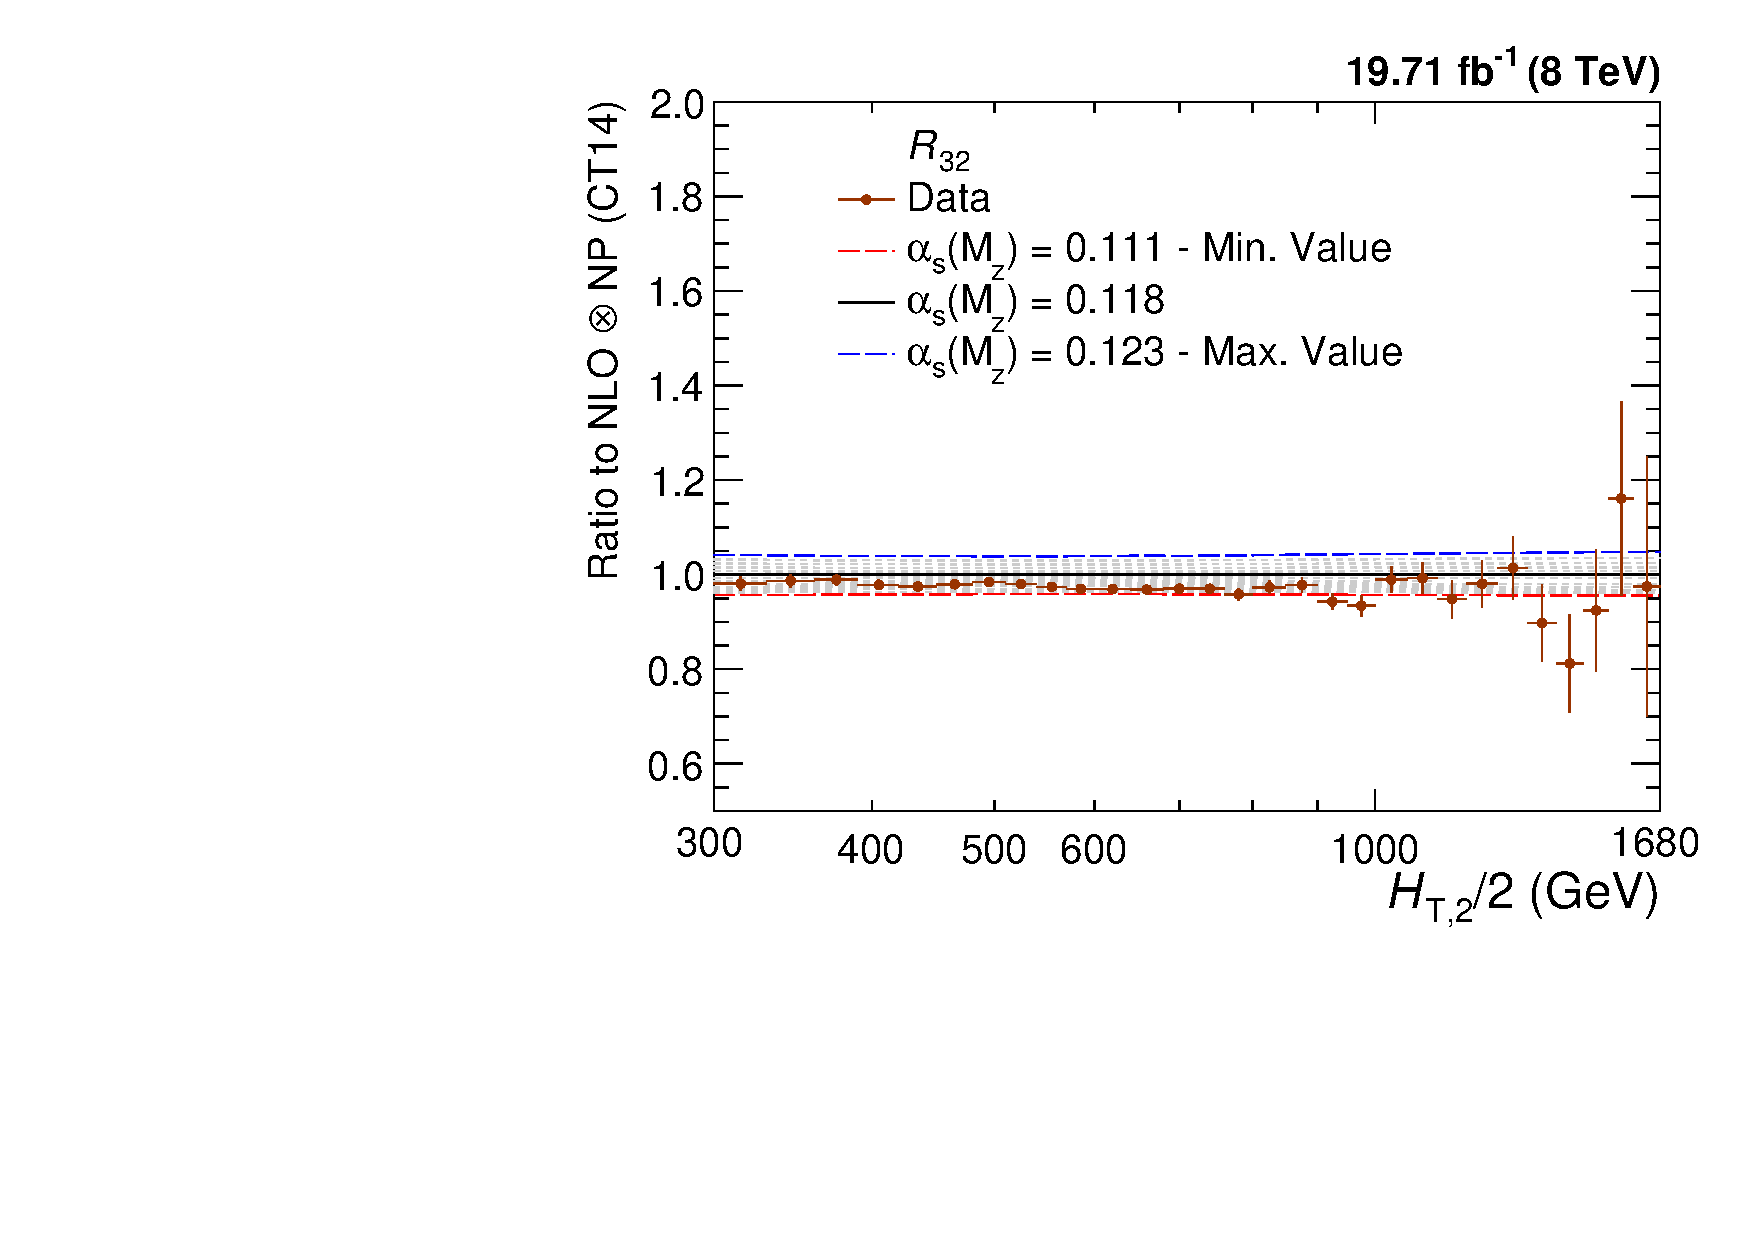
\includegraphics[scale = 0.207]{Plots_HT_2_150/Sensitivity_double_ratio_32_CT14.pdf}%
\includegraphics[scale = 0.207]{Plots_HT_2_150/Sensitivity_double_ratio_32_MSTW2008.pdf}\\
\vspace{5mm}
\includegraphics[scale = 0.207]{Plots_HT_2_150/Sensitivity_double_ratio_32_MMHT2014.pdf}%
\hspace{0.3mm}
\includegraphics[scale = 0.207]{Plots_HT_2_150/Sensitivity_double_ratio_32_NNPDF23.pdf}
\end{center}
\end{frame}

%##################################### Slide : ###########################################
\begin{frame}
\frametitle{\centerline{Strong Coupling Constant \alps}}
\label{alpha}
\setlength\labelsep   {\dimexpr\labelsep + 0.05em\relax}
\setlength\leftmargini{\dimexpr\leftmargini + 0.05em\relax}
\begin{center}
\begin{itemize}
\item {\scriptsize {\bf Inclusive jet [JHEP 03 (2017) 156] :} \\}
\tri
\begin{itemize}
\item {\scriptsize Least square minimization on \pt($y$) spectrum using NLO parton level predictions 
\vspace{2mm}
\item Using the CT10 NLO PDF set \\}
\end{itemize}
{\scalebox {0.85}{$\rm {\bf {\blue {\alpsmz = 0.1164\,^{+0.0014}_{-0.0015}\,\textrm{(exp)}\,^{+0.0025}_{-0.0029}\,\textrm{(PDF)}\,\pm0.0001\,\textrm{(NP)}\,^{+0.0053}_{-0.0028}\,\textrm{(scale)}}}}$}}\\
\vspace{1mm}	
\ball
\item {\scriptsize {\bf Multijets [CMS-PAS-SMP-16-008] :}\\}
\tri
\begin{itemize}
\item {\scriptsize 3-jet to 2-jet cross-section ratio, \ratio $\propto$ \alps
\vspace{2mm}
\item Insensitive to many theoretical and experimental systematics. 
\vspace{2mm}
\item Using the MSTW2008 PDF set \\}
\end{itemize}
{\scalebox {0.85} {$\rm {\bf {\blue {\alpsmz = 0.1150\,\pm0.0010\,\textrm{(exp)}\,\pm0.0013\,\textrm{(PDF)}\,\pm0.0015\,\textrm{(NP)}\,^{+0.0050}_{-0.0000}\,\textrm{(scale)}}}}$}}\\
\vspace{1mm}
\ball
\item {\scriptsize {\bf Triple differential dijets [EPJC 77 (2017) 746] :}\\}
\tri
\begin{itemize}
\item {\scriptsize Precise \alps extraction together with PDF fit \\}
\end{itemize}
{\scalebox {0.85} {$\rm {\bf {\blue {\alpsmz = 0.1199\,\pm0.0015\,\textrm{(exp)}\,\pm0.0002\,\textrm{(mod)}\,^{+0.0002}_{-0.0004}\,\textrm{(par)}\,^{+0.0031}_{-0.0019}\,\textrm{(scale)}}}}$}}\\
\ball
\end{itemize}
\end{center}
\end{frame}

\end{document}
